%%%%%%%%%%%%%%%%%%%%%%%%%%%%%%%%%%%%%%%%%%%%%%%%%%%%%%%%%%%%%%%%%%% 
%                                                                 %
%                            ROOT FILE                            %
%                                                                 %
%%%%%%%%%%%%%%%%%%%%%%%%%%%%%%%%%%%%%%%%%%%%%%%%%%%%%%%%%%%%%%%%%%% 
%
%  Run LaTeX or pdfLaTeX on this file to produce your thesis.
%  To produce the abstract title page followed by the abstract,
%  see the file abstitle-phd.tex or abstitle-mas.tex.
%
%%%%%%%%%%%%%%%%%%%%%%%%%%%%%%%%%%%%%%%%%%%%%%%%%%%%%%%%%%%%%%%%%%%

\documentclass[chap]{thesis}
\usepackage{textcomp}
\usepackage{amsmath,amssymb,amsfonts}
\usepackage[toc,page]{appendix}
\usepackage{graphicx}
\usepackage{xcolor}
\usepackage{array}
\usepackage{nicefrac}
\usepackage{adjustbox}
\usepackage{multirow}
% \usepackage{appendix}
\usepackage{multicol}
\usepackage{amsbsy}
% \PassOptionsToPackage{hyphens}{url}
\usepackage{hyperref}
\usepackage{url}
% \PassOptionsToPackage{hyphens}{url}\usepackage{hyperref}
% \usepackage[nobiblatex]{xurl}
\usepackage{mathtools}
% \usepackage[hyphenbreaks]{breakurl}
\usepackage{listings}
\usepackage{xspace}
\usepackage{attrib}
\usepackage{color}
\usepackage{dsfont}
\usepackage{placeins}
\usepackage{array}
\usepackage{caption}
\usepackage{fancyhdr}
\usepackage{booktabs}
\usepackage{tabularx}
% \usepackage{caption}
% \usepackage[font=small,labelfont=bf]{caption}
% \usepackage{enumitem}
\usepackage{geometry}
\usepackage{comment}
\usepackage{algorithm}
% \usepackage{algorithmic}
\usepackage{algpseudocode}
\usepackage{syntax}
\usepackage{amsthm}
\usepackage[bottom]{footmisc}
\usepackage{float}
\usepackage{titlesec}
\usepackage{environ} 
\floatstyle{plaintop}
\restylefloat{table}

\captionsetup{format=hang}


\usepackage[square,numbers]{natbib}

\titleformat{\subsubsection}
  {\bfseries\itshape}{\thesubsubsection}{1em}{}

\NewEnviron{SMALLEQ}{% 
    \scalebox{0.93}{$\BODY$} 
} 

\newcommand{\f}{{\sf f}\xspace}
\newcommand{\sss}{{\sf s}\xspace}
\newcommand{\nnn}{{\sf n}\xspace}
\newcommand{\iii}{{\sf i}\xspace}
\newcommand{\ccc}{{\sf c}\xspace}
\newcommand{\m}{{\sf m}\xspace}
\newcommand{\n}{{\sf n}\xspace}
\newcommand{\p}{{\sf p}\xspace}
\newcommand{\w}{{\sf {w}}\xspace}
\newcommand{\x}{{\sf {x}}\xspace}
\newcommand{\y}{{\sf y}\xspace}
\newcommand{\X}{{\sf {X}}\xspace}
\newcommand{\Y}{{\sf Y}\xspace}
\newcommand{\z}{{\sf z}\xspace}
\newcommand{\varv}{{\sf v}\xspace}
\newcommand{\D}{{\sf D}\xspace}
\newcommand{\new}{{\sf new}\xspace}
\newcommand{\this}{{\sf this}\xspace}
\newcommand{\unit}{{\sf unit}\xspace}
\newcommand{\ret}{{\sf ret}\xspace}

% macros for reference (ana)
% \newcommand\secref[1]{Sect.~\ref{#1}}
% \newcommand\figref[1]{Fig.~\ref{#1}} 
\newtheorem{definition}{Definition}
\newtheorem{theorem}{Theorem}
\newtheorem{lemma}{Lemma}
\theoremstyle{definition}
\newtheorem{remark}{Remark}
\newtheorem{assumption}{Assumption}
\newtheorem{problem}{Problem}

\newcommand{\op}{{\sf aop}\xspace}
\newcommand{\cop}{{\sf bop}\xspace}
\newcommand{\ol}[1]{\overline{#1}}
\newcommand{\code}[1]{{\sf #1}\xspace}
\newcommand{\squad}{\;\;\;}
\newcommand{\trule}[1]{\textsc{\scriptsize ({#1})}}

\newcommand\attribfootnote[1]{%
 \begingroup
 \renewcommand\thefootnote{}\footnote{#1}%
 \addtocounter{footnote}{-1}%
 \endgroup
}

\newcommand{\todoana}[1]{{\color{blue}\bfseries [#1]}}
\newcommand{\todolindsey}[1]{{\color{red}\bfseries [#1]}}
\newcommand{\ana}[1]{\todoana{Ana: #1}}
\newcommand{\lindsey}[1]{\todolindsey{Lindsey: #1}}
\newcommand*{\Z}{\mathds{Z}}
\newcommand\secref[1]{Sect.~\ref{#1}}
\newcommand\figref[1]{Fig.~\ref{#1}}
\newcommand\chapref[1]{Chap.~\ref{#1}}
\newcommand\defref[1]{Def.~\ref{#1}}
\newcommand\tabref[1]{Tab.~\ref{#1}}
\newcommand\trmref[1]{Thm.~\ref{#1}}
\renewcommand\algref[1]{Alg.~\ref{#1}}
\newcommand\lemref[1]{Lemma~\ref{#1}}
\newcommand\problemref[1]{Problem~\ref{#1}}
\newcommand{\boldphi}{\boldsymbol{\phi}}


\newcommand{\A}{{\sf A}}
\newcommand{\B}{{\sf B}}
\newcommand{\C}{{\sf C}}
% \renewcommand{\theenumi}{\Roman{enumii}}

\renewcommand\bibname{REFERENCES} % specify name of your heading


\lstdefinestyle{javastyle} {
    basicstyle=\sffamily\footnotesize,
    frame=single,
    numbers=left,
    tabsize=2,
    language=Java,
    columns=fullflexible,
    escapechar=?,
    keepspaces=true,
    showstringspaces=false,
    breakatwhitespace=false,
    captionpos=b,  
    morekeywords={Integer,List,Text, Phi},
    escapeinside={(*@}{@*)}
}

\lstdefinestyle{pythonstyle} {
    basicstyle=\sffamily\footnotesize,
    frame=single,
    numbers=left,
    tabsize=2,
    language=Python,
    columns=fullflexible,
    escapechar=?,
    keepspaces=true,
    showstringspaces=false,
    breakatwhitespace=false,
    captionpos=b,  
    morekeywords={Integer,List,Text, Phi},
    escapeinside={(*@}{@*)}
}

\lstnewenvironment{javacode}
{\lstset{style=javastyle}}
{}

\lstnewenvironment{pythoncode}
{\lstset{style=pythonstyle}}
{}

\def\BibTeX{{\rm B\kern-.05em{\sc i\kern-.025em b}\kern-.08em
    T\kern-.1667em\lower.7ex\hbox{E}\kern-.125emX}}

\graphicspath{ {images/} }

\newenvironment{semantics}{
    \begin{displaymath}}{
    \end{displaymath}
}
% Uncomment the following if you want centered-lined captions:
%\captionsetup{format=plain,justification=centering}


%\includeonly{rpichap1}  % use \includeonly to process only
                         % the file(s) listed inside the braces        
               
\begin{document}
 
% Use the appropriate example title page.  A senior thesis
% can be set by changing the thesis name in rpititle-mas.tex.
%\include{title}   % titlepage material for PhD thesis 
%\include{rpititle-mas}   % titlepage material for Master thesis 
%\include{acknowledgments}  % include for acknowledgements
%\include{abstract} % abstract
%\include{chapterone} % chapter 1
%\include{chaptertwo} % chapter 2
%\include{chapterthree} % chapter 3
%%%%%%%%%%%%%%%%%%%%%%%%%%%%%%%%%%%%%%%%%%%%%%%%%%%%%%%%%%%%%%%%%%% 
%                                                                 %
%                            CHAPTER FOUR                         %
%                                                                 %
%%%%%%%%%%%%%%%%%%%%%%%%%%%%%%%%%%%%%%%%%%%%%%%%%%%%%%%%%%%%%%%%%%% 

%\begin{document}
 
\chapter{MPC AMORTIZATION: SCHEDULING FOR MPC LOOPS}
\label{chapter:chapterfour}
\resetfootnote %this command starts footnote numbering with 1 again.

\section{Introduction}
\label{sec:intro}

%\ana{Lindsey, look at the figures to format some of them and put the period at the end of the caption if it's missing.}

As the demand for cloud computation has increased so has the demand for secure solutions 
for cloud platforms. In the last decade cloud serves have become an almost \$100 billion industry. 
\cite{Synergy2019}. This high consumer demand, as well as the need for high security within these
frameworks has fueled research into varying cryptographic concepts like Multiparty Computation and 
Homomorphic Encryption. 

Researchers have proposed different encryption schemes to support 
a variety of operations, allowing for larger and larger subsets of
programs to be run this way. Again, Fully Homomorphic Encryption (FHE) \cite{Gentry:2010},\cite{Gentry:20102}  
can perform arbitrary operations on encrypted data, but in its current state FHE
is still prohibitively expensive \cite{Gentry:2011}. An alternative to FHE 
is Partially Homomorphic Encryption (PHE), which scales substantially better, but cannot 
perform arbitrary operations, and requires the conversions. %that were discussed in \chapref{chapter:chapterthree}.

As we discussed earlier, Multiparty Computation (MPC) describe groups of protocols that can be used in secure collaborative
computation. MPC benefits from having high security stemming from extensive theoretical guarantees. 
%without having to resort to expensive
%solutions (like FHE) or solutions with lower security (PHE conversion). 

Within MPC certain optimizations can be made in the evaluation of loops bodies. Due to the transformation of problems into an 
intermediate representation, similar operations within an MPC problem can be amortized. %, or performed in parallel, 
%with little drawbacks as long as certain assumptions hold. 
We present a technique for automatically locating opportunities for amortization to improve performance in compiled MPC programs. 

The rests of this chapter is organized as follows: \secref{sec:mpcoverview}, provides a brief over view of our work. 
\secref{sec:language} shows our language specification.
\secref{sec:parallelization} briefly outlines outlines dependenceies, and describes HPC Parallelizion as well as 
MPC Amortization in \secref{sec:hpcparallelization} and \secref{sec:mpcamortization}. 
\secref{sec:loopbodyanalysis} and \secref{sec:analysis} show our analysis. \secref{sec:loopscheduling} 
presents our scheduling algorithms. \secref{sec:results} presents our empirical results. 
% Finally, \secref{sec:conclusions} concludes. 
%\ana{Broken links again here. I think this needs to be rewritten as we moved stuff into Chapter 2.} \lindsey{fixed!}

\section{Overview}
\label{sec:overview}


\begin{table*}
\begin{tabular}{ccc}
\begin{minipage}{0.275\textwidth}
{\small
\begin{pythonn}
def biometric(C: shared[list[int]], D: int,
      S: shared[list[int]], N: int) ->
      shared[tuple[int,int]]:
   min_sum : int = MAX_INT
   min_idx : int = 0
   for i in range(N):
      sum : int = 0
      for j in range(D):
         # d = S[i,j] - C[j]
         d : int = S[i * D + j] - C[j]
         p : int = d * d
         sum = sum + p
      if sum < min_sum:
         min_sum : int = sum
         min_idx : int = i
   return (min_sum, min_idx)
\end{pythonn}
}
\end{minipage}

&

\begin{minipage}{0.33\textwidth}
{\tiny
\begin{pythonn}
min_sum!1 = MAX_INT
min_idx!1 = 0
for i in range(0, N):
   min_sum!2 = PHI(min_sum!1, min_sum!4)
   min_idx!2 = PHI(min_idx!1, min_idx!4)
   sum!2 = 0
   for j in range(0, D):
      sum!3 = PHI(sum!2, sum!4)
      d = SUB(S[((i * D) + j)],C[j])
      p = MUL(d,d)
      sum!4 = ADD(sum!3,p)
   t = CMP(sum!3,min_sum!2)
   min_sum!3 = sum!3
   min_idx!3 = i
   min_sum!4 = MUX(t, min_sum!3, min_sum!2)
   min_idx!4 = MUX(t, min_idx!3, min_idx!2)
return (min_sum!2, min_idx!2)
\end{pythonn}
}
\end{minipage}

&

\begin{minipage}{0.33\textwidth}
{\small
\begin{pythonn}
min_sum!1 = MAX_INT
min_idx!1 = 0
# S^ is same as S. C^ replicates C N times:
S^ = raise_dim(S, ((i * D) + j), (i:N,j:D)) #S^[i,j] = S[i,j]
C^ = raise_dim(C, j, (i:N,j:D)) #C^[i,j] = C[j]

sum!2[I] = [0,..,0]
# computes _all_  "at once"
d[I,J] = SUB_SIMD(S^[I,J],C^[I,J])
p[I,J] = MUL_SIMD(d[I,J],d[I,J])

for j in range(0, D):
   # sum!2[I], sum!3[I], sum!4[I] are size-N vectors
   # computes N intermediate sums "at once"
   sum!3[I] = PHI(sum!2[I], sum!4[I])
   sum!4[I] = ADD_SIMD(sum!3[I],p[I,j])

min_idx!3[I] = [0,1,...N-1]
for i in range(0, N):
   min_sum!2 = PHI(min_sum!1, min_sum!4)
   t[i] = CMP(sum!3[i],min_sum!2)
   min_sum!4 = MUX(t[i], sum!3[i], min_sum!2)
for i in range(0, N):
   min_idx!2 = PHI(min_idx!1, min_idx!4)
   min_idx!4 = MUX(t[i], min_idx!3[i], min_idx!2)
return (min_sum!2, min_idx!2)
\end{pythonn}
}
\end{minipage}

\\

(a) IMP Source & (b) MPC Source & (c) Optimized MPC Source
\end{tabular}
\caption{Biometric Matching: ==== From (a) IMP Source to (b) MPC Source: 
First, MPC Source is an SSA form.
Second, it is linear. The conditional in lines 13-14 in IMP Source turns into the linear code in lines 12-16 in MPC Source.
The test turns into the CMP operation {\sf t = CMP(sum!3,min\_sum!2)}, followed by the
true-branch sequence, followed by the MUX operations. The first MUX operation selects the value
of {\sf min\_sum}: if {\sf t} is true, then {\sf min\_sum} gets the value of the second multiplexer
argument,  {\sf min\_sum!3}, otherwise it takes the value of the third argument, {\sf min\_sum!2}.
Third, MPC Source is a special form of SSA. The SSA $\phi$-nodes at the if-then-else (lines 13-15) turn into
MUX operations, while the $\phi$-nodes at for-loops turn into \emph{pseudo} PHI nodes with a straightforward semantics.
==== From (b) MPC Source to (c) Optimized MPC Source: 
The compiler determines that SUB and MUL in ``naive'' MPC Source (lines 9 and 10 in (b))
can be fully vectorized into the SIMD SUB and MUL in optimized MPC Source (lines 9 and 10 in (c)).
Notation {\sf p[I,J]} denotes a 2-dimensional array with fully vectorized dimensions.
The computation of sum (line 11 in (b))
is sequential across the $j$-dimension, but it is parallel across the $i$-dimension.
The loop in lines 12-16 in (c) illustrates; here {\sf p[I,j]} refers to the $j$-th column in {\sf p}.
Unfortunately, CMP and MUX remain sequential.
% \ana{Add explanation to caption, this is hard to see.}
}
\label{tab:source_and_MPC_source_and_optimized_MPC_source}
\end{table*}


\subsection{Source}

As a running example, consider Biometric matching, a standard MPC benchmark.
An intuitive (and naive) implementation is as shown in Listing~\ref{tab:source_and_MPC_source_and_optimized_MPC_source}(a).
Array {\sf C} is the feature vector of {\sf D} features that we wish to match and {\sf S}
is the database of {\sf N} size-{\sf D} vectors that we match against.

Our compiler takes essentially standard IMP~\cite{Nipkow2014}
syntax and imposes certain semantic restrictions. %(We detail the restrictions in the following sections.)
The programmer writes an iterative program and annotates certain inputs
and outputs as \emph{shared}. In the example arrays {\sf C} and {\sf S}
are \texttt{shared}, meaning that they store shares, however, the array sizes {\sf D} and
{\sf N} respectively are plaintext. 
%The code iterates over the entries in the
%database and computes the Euclidean distance of the current
%entry ${\sf S}[i]$ and {\sf C} (its square actually). The program returns the index of the vector that gives
%the best match plus the corresponding sum of squares.

\subsection{MPC Source and Cost of Schedule}

Our compiler generates an intermediate representation, MPC Source. 
MPC Source is a \emph{linear} SSA form.
MPC Source for Biometric Matching is shown and described in detail in
Listing~\ref{tab:source_and_MPC_source_and_optimized_MPC_source}(b). 


\begin{comment}
First, MPC Source is an SSA form.
Second, it is linear. The conditional in lines 13-14 in IMP Source turns into the linear code in lines 12-16 in MPC Source.
The test turns into the CMP operation {\sf t = CMP(sum!3,min\_sum!2)}, followed by the
true-branch sequence, followed by the MUX operations. The first MUX operation selects the value
of {\sf min\_sum}: if {\sf t} is true, then {\sf min\_sum} gets the value of the second multiplexer
argument,  {\sf min\_sum!3}, otherwise it takes the value of the third argument, {\sf min\_sum!2}.
Third, MPC Source is a special form of SSA. The SSA $\phi$-nodes at the if-then-else (lines 13-15) turn into
MUX operations, while the $\phi$-nodes at for-loops turn into \emph{pseudo} PHI nodes with a straightforward semantics.
\end{comment}

We turn to our analytical model to compute the \emph{cost} of the iterative program. Assume
cost $\beta$ for a local MPC operation (e.g., ADD in Arithmetic sharing) and cost $\alpha$ for a remote
MPC operation (e.g., MUX, CMP, etc.). Assuming that ADD is $\beta$ and SUB, CMP and MUX are $\alpha$, 
the MPC Source in Listing~\ref{tab:source_and_MPC_source_and_optimized_MPC_source}(b) gives 
rise to an iterative schedule with cost $ND(2\alpha+\beta) + N(3\alpha$).

A key contribution is the vectorizing transformation. We can compute all $N*D$
subtractions (line 9 in (b)) in a single SIMD instruction; similarly we can compute
all multiplications (line 10) in a single SIMD instruction. And while computation
of an individual sum remains sequential, we can compute the $N$ sums in parallel.
%Our compiler \emph{automatically detects these opportunities and transforms the program}.
%It is standard that MPC researchers write vectorized versions of the Biometric
%program by hand; we are the first (to the best of our knowledge) to automatically
%transform a naive, iterative MPC program into an unintuitive vectorized one.

\subsection{Vectorized MPC Source and Cost of Schedule}

Our compiler produces the vectorized program shown and described in 
Listing~\ref{tab:source_and_MPC_source_and_optimized_MPC_source}(c).
Note that this is still our intermediate representation, Optimized MPC Source. Subsequently,
the compiler turns this code into MOTION variables, loops and SIMD primitives, which MOTION then
uses to generate the circuit.
\begin{comment}
The compiler determines that SUB and MUL in ``naive'' MPC Source (lines 9 and 10 in (b))
can be fully vectorized into the SIMD SUB and MUL in optimized MPC Source (lines 9 and 10 in (c)).
Notation {\sf p[I,J]} denotes a 2-dimensional array with fully vectorized dimensions.
The computation of sum (line 11 in (b))
is sequential across the $j$-dimension, but it is parallel across the $i$-dimension.
The loop in lines 12-16 in (c) illustrates; here {\sf p[I,j]} refers to the $j$-th column in {\sf p}.
Unfortunately, CMP and MUX remain sequential.
\end{comment}

In MPC back ends, executing $n$ operations ``at once'' in a single SIMD operation costs a lot less than executing those $n$ operations one by one.
This is particularly important when there is communication (i.e., in remote), since many 1-bit values are sent at once rather than sequentially.
%In MPC compilers a vectorized operation that computing M operations "at once" costs
%essentially the same ($\alpha$ or $\beta$) as an individual operation.
We elaborate on the cost model in Section~\secref{sec:model} but for now consider that
each operation has a \emph{fixed} portion (does benefits from amortization) and
a \emph{variable} portion (does not benefit from amortization): $\alpha = \alpha_\mathit{fix} + \alpha_\mathit{var}$.
This gives rise to the following formula for amortized cost: $f(n) = \alpha_\mathit{fix} + n\alpha_\mathit{var}$,
as opposed to unamortized cost $g(n) = n\alpha_\mathit{fix} + n\alpha_\mathit{var}$. We extend the same reasoning to
$\beta$-instructions.

Thus, the fixed cost of the vectorized program amounts to
$2\alpha_\mathit{fix}$ + $D \beta_\mathit{fix} + N(3\alpha_\mathit{fix})$. (The variable cost is the same in both the vectorized and non-vectorized programs.)
The first term in the sum corresponds to the vectorized
subtraction and multiplication (lines 9-10 in (c)), the second term corresponds to the for-loop on $j$ (lines 12-16) and the third
one corresponds to the remaining for-loops on $i$ (lines 19-25). 
Clearly, $2\alpha_\mathit{fix} + D\beta_\mathit{fix} + N(3\alpha_\mathit{fix}) << ND(2\alpha_\mathit{fix}+\beta_\mathit{fix}) + N3\alpha_\mathit{fix}$.
Empirically, we observe that (1) $\alpha_\mathit{var} \approx 0$ and (2) there is orders of magnitude improvement in running time and memory. 
E.g., we see about 12x improvement in online time in GMW for $N=128$. Additionally, the non-vectorized version runs out of memory for $N=256$, 
while the vectorized one runs with the standard maximal input size $N=4,096$.
%\ana{Edit numbers with final experiments.}

\section{Language Specification}
\label{sec:language}

We start with an IMP-like \cite{Nipkow2014} language, syntactically similar to imperative
C-style languages (C, C++, Java, C\#, etc.). %\ana{What's this ref to?}\lindsey{my mistake, to nothing removed.} 
We restrict our language by disallowing recursion, and assuming that all loop bounds are both known and static. 
% This leaves us with a general language syntax as shown in \figref{fig:impsyntax}.
Next the program is converted to SSA using a modified version of the algorithms of 
Cytron et al. \cite{Cytron1991}. Those algorithms have two main steps: the creation
of $\phi()$ functions at merge points in the program, and the renaming of variables
to ensure that every variable is only on the left hand side of an assignment statement once.
Crucially during our transformation merges between two blocks that contain different variable
versions are not transformed into $\phi()$ nodes but are instead converted to MUX gates. This
prevents data leakage due to observations of program execution. Once in this form loop 
bodies can be unrolled, allowing the MPC compiler to create a circuit 
representation of the program. Our language is similar to recent work
in the MPC literature that optimizes protocol selection during 
compilation \cite{Ishaq2019}. \figref{fig:muximpsyntax} shows our output syntax. 
We assume standard scalar variables (i.e. $\x$, $\y$, ${\sf c}$) and array members (i.e. ${\A[i]}$) are sensitive 
values, while looping variables and variables that represent loop bounds (i.e. $N$, $i$) are known at compile time.
All functions in our language can be vectorized. This means that any function in our language 
(i.e. ADD) can be computed on two arrays for the same cost as computing the same 
function of two scalar values.
%\ana{This last sentence is unclear, try to rewrite.}
%\lindsey{better?}
% However, as stated above, do not include $\phi()$ functions directly 
% and convert if statements to MUX nodes.


% \begin{figure}
% \small
% \[
% \begin{array}{l@{~~~~~}l}
%   \begin{array}{l@{~}l@{~~~}l}
%   s & ::= s ; s \\ 
%   & \mid \x = \y  \\
%   & \mid \x=\y \; \op \; \z \\
%   & \mid {\sf A}[i] = \x \\
%   & \mid \x = \A[i] \\
%   & \mid {\sf for} \; (i = 0; i \le n; \mathit{i\!+\!+}) \; \{ \; s \; \} \\
%   & \mid {\sf if} \; (\x \; \cop \; \y) \; \{ \; s \; \} \; {\sf else} \; \{ \; s \; \} \; & \mathit{statement} \\ 
%   \op &::= + \mid - \mid * \mid / & \mathit{arithmetic} \; \mathit{operator} \\
%   \cop &::=  \; == \; \mid \; != \; \mid \; < \; \mid \; \le & \mathit{comparison} \; \mathit{operator}

%   \end{array}
% \end{array}
% \]
% %\vspace{-0.2in}
% \caption{Source IMP syntax as defined in \cite{Nipkow2014}: \sss is a sequence of statements. 
% \x, \y, \z, \iii, and \nnn are variables.} 
% \label{fig:impsyntax}
% \end{figure}

\begin{figure}
\small
\[
\begin{array}{l@{~~~~~}l}
  \begin{array}{l@{~}l@{~~~}l}
  s & ::= s ; s \\ 
  & \mid \x = \y  \mid \x = p \mid \A[i] = \x \mid \x = \A[i] \\
  & \mid \A[f(i)] = \x \; \mid \x = \A[f(i)] 
  \end{array}
\end{array}
\begin{array}{l@{~~~~~}l}
  \begin{array}{l@{~}l@{~~~}l}  
  p &  ::= {\sf ADD(x, y) \mid ADD\_N(X, Y, n)} & \mathit{primitive} \\ 
  & \mid {\sf SUB(x, y) \mid SUB\_N(X, Y, n)} &  \\ 
  & \mid {\sf MUL(x, y) \mid MUL\_N(X, Y, n)} &  \\ 
  & \mid {\sf CMP(x, y) \mid CMP\_N(X, Y, n)} &  \\ 
  & \mid {\sf XOR(x, y) \mid XOR\_N(X, Y, n)} &  \\ 
  & \mid {\sf SHL(x, y) \mid SHL\_N(X, Y, n)} &  \\ 
  & \mid {\sf SHR(x, y) \mid SHR\_N(X, Y, n)} &  \\ 
  & \mid {\sf REM(x, y) \mid REM\_N(X, Y, n)} & \\ 
  & \mid {\sf OR(x, y)  \mid OR\_N(X, Y, n)} &  \\ 
  & \mid {\sf AND(x, y) \mid AND\_N(X, Y, n)} &  \\ 
  & \mid {\sf MUX(x, y, c) \mid MUX\_N(X, Y, c, n)} &  \\ 
  \end{array}
\end{array}
\]
%\vspace{-0.2in}
\caption{Target MPC syntax: $s$ is a straight-line sequence of statements. 
\x, \y, and {\sf i} are variables, {\A}, \X, and \Y are arrays. $p$ is what we call an MPC primitive. 
\n is the length of the arrays passed to parallel functions. This means that
ADD, SUB, MUL, CMP, XOR, SHL, SHR, REM, OR, AND, and MUX are functions on scalar values, 
while ADD_N, SUB_N, MUL_N, CMP_N, XOR_N, SHL_N, SHR_N, REM_N, OR_N, AND_N, and MUX_N are parallel functions on arrays.
Our analysis takes a high-level C-like program and outputs a (potentially vectorized) in this low-level target language.
%\ana{Change font for x and y, as in the other syntax figure.}\lindsey{fixed!}
%\ana{I'm having hard time remembering what we had in mind with this figure... This was the target MPC code, right?}
%\ana{If yes, then remove the for loop. There is no for loop in MPC code, we just unrol.}
%\ana{TODO, ANA: I think here we might have to introduce the parallel MUX, AND, etc.,} \lindsey{fixed!}
}
\label{fig:muximpsyntax}
\end{figure}


\section{Parallelization}
\label{sec:parallelization}

\subsection{Loop Dependencies} 
\label{sec:loopdependencies}

Array loop optimization is a crucial component of compiler design. More specifically
the optimizations that can be done on arrays \emph{within} a loop make better use of 
parallelization which results in decreased running times. The effectiveness of the 
optimization is entirely dependent on two factors: the number of processing threads
available, and the dependencies between the statements of the loop. These dependencies 
come in two types: Control-dependencies and data-dependencies. Control dependencies
exist between statements where the control flow of the program determines
program execution. Data-dependencies are dependencies that exist 
between nodes based on their interaction with shared data.

Aiken et al. \cite{Aiken1988} provides an illustration of data-dependencies. 
Consider the code in \figref{fig:arrayloop}. Line 2 is not dependent on any other 
line calculated in the same iteration. Line 5 is dependent on the calculation 
of lines 3, and 4. More interestingly lines 3, 4 are not only dependent on line 2, 
but also on a \emph{previous calculation} of line 5. 

\begin{figure}[h]
\centering
\begin{minipage}{0.70\textwidth}
\begin{javacode}
	for(int i = 0; i < N; i++) {
		A[i] = B[i];
		B[i] = A[i] * D[i - 1];
		C[i] = A[i] * D[i - 1];
		D[i] = B[i] * C[i]; 
	}
\end{javacode}
\end{minipage}
\caption{Loop containing array dependencies, a modified example from Aiken et al. \cite{Aiken1988}.}
\label{fig:arrayloop}
\end{figure}

\begin{figure}[h]
\centering
\begin{minipage}{0.70\textwidth}
\begin{javacode}
  if(<Cond1>) {
      <Stmt1>
  } else if(<Cond2>) {
      <Stmt2>
  } else {
      <Stmt3>
  }
\end{javacode}
\end{minipage}
\caption{If-Then-Else dependency.}
\label{fig:ifthenelsedep}
\end{figure}


Every data-dependency either effects variables within the current loop iteration
(intra-loop dependency) or effects variables on a different loop iteration
(across-loop dependency). One type of simple across-loop dependency occurs when a single
variable is modified by a previous calculation of itself. This is a trivial case,
but still counts as an across-loop dependency. Data dependences are preserved in the 
transformation to target MPC code. 


The most common type of control-dependency is the If-Then-Else dependency shown
in \figref{fig:ifthenelsedep}. The execution of each statement is dependent on the various conditionals 
present. In this example all three statements are dependent on the outer if conditional while only
statements 2 and 3 are dependent on inner conditional. Control dependences 
are ``inverted'' in the target MPC code. Instead of dependencies between the branch statements
to the conditional, there will be a dependence from statement 2 and 3 to the MUX 
node, as well as a dependecy between the MUX node and the conditional. 

\subsection{HPC Parallelization}
\label{sec:hpcparallelization}

In the High performance computing (HPC) world a schedule is created to minimize the number
of sequential instructions of a program by utilizing a fixed number of threads. There 
are two main factors that determine the extent to which optimization can take place.
The first are control and data dependencies discussed above. The second is the number
of parallel processes that can be executed (i.e. the number of threads available). 
Importantly, each thread can perform arbitrary operations that are not reliant on the operations 
run on any other thread. The optimal schedule is then that which achieves the minimum number 
of sequential steps, while both preserving inter-loop and cross-loop dependencies 
and maximizing resource use. 
% In HPC optimizations \ana{Incomplete sentence?}.

Schedules are evaluated based off of their maximum \emph{delay}. The delay of a given 
schedule represents the number of steps between loop iterations that are 
carried out to preserve all looping dependencies \cite{Aiken1988}. 
For example, a variable modifying itself within a loop has a static distance of 1
iteration between the definition and usage. Creating a schedule with an optimal minimal delay
(steps between loop iterations) with a restricted number of processors has been shown to be
NP-hard \cite{Cytron1984},\cite{Graham1971},\cite{Darte2000}. 
Modern compilers often use heuristics to achieve a schedule
that is as close to optimal as possible. The classical HPC literature 
has considered different types of across-loop scheduling schemes. 
One scheduling scheme, called \emph{doacross}~\cite{Aiken1988},\cite{Cytron1986}, requires that all instructions in an 
iteration are scheduled on the same processor. 
The optimal doacross schedule for \figref{fig:arrayloop} (from \cite{Aiken1988}) is shown in \figref{fig:HPCexample} (b). 
Next, Aiken and Nicolau \cite{Aiken1988} proposed a new schedule, which they called
\emph{greedy} schedule, where instructions in an iteration can be scheduled on different processors. 
The optimal greedy schedule for our example, which achieves better minimal delay than the optimal 
doaccross schedule, is shown in \figref{fig:HPCexample}(c) (again, taken directly from~\cite{Aiken1988}). 

\begin{figure*}[tbhp]
\small
\begin{tabular}{lll}


\begin{minipage}[b]{4.20cm}
\centering
\includegraphics[width=0.4\textwidth]{images/HPCloop.pdf}
\end{minipage}

&

\begin{minipage}[b]{4.20cm}
\centering
\includegraphics[width=0.4\textwidth]{images/HPCdoacrossLoop.pdf}
\end{minipage}

&

\begin{minipage}[b]{4.20cm}
\centering
\includegraphics[width=0.6\textwidth]{images/HPCgreedyLoop.pdf}
\end{minipage}

\\

(a) Loop-body schedule
&
(b) Doacross across-loop schedule
& 
(c) Greedy across-loop schedule

\end{tabular}
\caption{Optimal HPC schedules. Different statements are each given letters. 
In (a) only one loop iteration is shown. In (b) and (c) variables 
are labeled according to both their statement (i.e A, B, C) and the loop iteration that is being 
computed which is shown in parentheses (A(1) represents the statement A on iteration 1).}
\label{fig:HPCexample}\vspace{-2ex}
\end{figure*}

\subsection{MPC Amortization}
\label{sec:mpcamortization} 

In MPC, the loop scheduling problem is different. Instead of having a fixed number of 
processors that carry out arbitrary independent operations, in MPC schedules the we assume that we can run
infinitely many operations (same operations) in parallel. We note that the relaxation of allowing infinite bandwidth 
is often made in the HPC setting as well and it is not necessarily valid in either case. 
Our current relies on this assumption however, in future work we plan to relax the 
assumption and extend our study and results.

%\lindsey{Ana, does something like this work? ``While there is still
%a practial limit to the number of operations that can be run in parallel it is not directly defined by the
%number of physical processors avaialable. We can also assume infinite processors in HPC, but this 
%fundamentally removes all constraits from the problem.'' This is to address wes's questions: We can do this in HPC waht is the diff}
%threads that can only run similar operations simultaneously.

For example, consider two separate operations A and B. We assume that both operations have 
the same constant running time. In classic HPC optimization both A and B can be run simultaneously with no 
restrictions as long as two processors are available to compute them. In MPC scheduling,
there is no restriction based on number of processors, but there is one on the types of
operations that are run in parallel. This means that there is only a benefit from amortization if A is run in parallel 
with another A operation, or B is run with another B operation. Our work aims to create a novel analysis 
that can be used to create schedules that improve the performance of MPC loops. 

% All similar operations  (in this case equality, 
% comparison, and subtraction) can be performed at the same cost as a single operation of that type. 

% \ana{Don't use the GCD example because it does not lend to parallelization. 
% Use the Aiken paper example, or the inner product example.}
% \figref{fig:gcdparallel}, shows a Java 8 examaple of how gcd() could be run in 
% parallel so each operation could benefit from amoritization. 

\begin{figure}[h]
\centering
\begin{minipage}{0.7\textwidth}
\begin{javacode}
  InnerProduct(A, B) {
      sum = 0;
      for(int i = 0; i < N; i++) {
          sum += A[i] * B[i];
      }
      return sum;
  }
\end{javacode}
\end{minipage}
\caption{Original inner product code.}
\label{fig:innerproduct}
\end{figure}

\begin{figure}[h]
\centering
\begin{minipage}{0.7\textwidth}
\begin{javacode}
  InnerProduct(A, B) {
      sum = 0
      for(int i = 0; i < N; i++) {
          tmp = MUL(A[i], B[i]);
          sum = ADD(sum, tmp);
      }
      return sum;
  }
\end{javacode}
\end{minipage}
\caption{MPC source for inner product.}
\label{fig:innerproductmpc}
\end{figure}

\begin{figure}[h]
\centering
\begin{minipage}{0.7\textwidth}
\begin{javacode}
  InnerProduct(A, B) {
      C = MUL(A, B, N)
      sum = 0
      for(int i = 0; i < N; i++) {
          sum = ADD(sum, C[i]);
      }
  }
\end{javacode}
\end{minipage}
\caption{Vectorized MPC source for inner product.}
\label{fig:innerproductmpcvec}
\end{figure}

\begin{figure}[h]
\centering
\begin{minipage}{0.7\textwidth}
\begin{javacode}
  int[][]  split_list(int[] A) {
      A = pad_array(A); // adds 0 to an odd length array
      int[][] B = new int[2][A.length / 2];
      for(int i = 0; i < A.length / 2; i++) {
          B[0][i] = A[2 * i];
          B[1][i] = A[(2 * i) + 1];
      }
      return B;
  }

  private static int  SUM(int[] A) {
      int[][] W = split_list(A);
      while(A.length > 1) {
          A = ADD_N(W[0], W[1]);
          W = split_list(A);
      }
      return A[0];
  }
  InnerProduct(A, B) {
      C = MUL(A, B, N)
      return SUM(C)
  }
\end{javacode}
\end{minipage}
\caption{Vectorized MPC source for inner product using divide and conquer.}
\label{fig:innerproductmpcvecdandc}
\end{figure}

\begin{figure}[h]
\centering
\begin{minipage}{0.7\textwidth}
\includegraphics[width=1\textwidth]{divideconquer}
\end{minipage}
\caption{An example of \figref{fig:innerproductmpcvecdandc} for $n = 8$. 
Each level of tree is executed in parallel. This reduces the run time 
complexity from $O(n)$ to $O(log_{2}(n))$.}
\label{fig:treeexample}
\end{figure}

\figref{fig:innerproduct}, \figref{fig:innerproductmpc}, and \figref{fig:innerproductmpcvec} 
show a full transformation from high-level C-like source that computes the inner produce of 2 arrays {\sf A} and {\sf B}, 
to a fully vectorized MPC source that can be turned into an optimal MPC schedule. \figref{fig:treeexample}
shows a visualization of the execution performed for $n = 8$.
Initially in \figref{fig:innerproduct} and \figref{fig:innerproductmpc} $N$ 
multiplications and additions are performed. However in \figref{fig:innerproductmpcvec} 
the multiplications can be flattened to one operation, while the
additions are still performed sequentially with a \emph{for} loop. In  \figref{fig:innerproduct} the time
complexity of the algorithm is $O(n)$ where $n$ is the length of the array. Removing
the multiplication from the loop body does not reduce the asymptotic complexity, however,
in practice this has significant impact as in MPC multiplication is an expensive operation that
requires remote computation of the parties while addition is local and inexpensive. 
In addition, vectorization of multiplication allows for the addition operation to be isolated and 
additionally optimized, using divide-and-conquer techniques, which reduces the complexity to
$O(log_2(n))$ \cite{Farzan2017}. The transformation for inner product is shown in \figref{fig:innerproductmpcvecdandc}.

The great benefit of MPC amortizations is, due to the circuit representation, there is no inherent 
limit of the scale of parallelization. As we mentioned in \secref{sec:hpcparallelization} general
scheduling is a NP-Hard problem \cite{Cytron1984},\cite{Graham1971} however this is due to the restrictions
on the number of processors, with an unlimited number of processors the problem can be solved in polynomial time
\cite{Darte2000}. We claim that our problem is substantially different. In summary, the MPC amortization problem 
is different from the HPC parallelization problem because: in MPC we can assume unlimited bandwidth, and also 
we can only ``schedule in parallel'' two operations that are the same; in HPC we have a fixed number of processors, 
and we can schedule in parallel any two operations. Thus, we avoid some of the limitations that are present in HPC 
scheduling, while MPC imposes its own limitations and constraints. 


This leads to our two main problems. 

\begin{problem}
Given a loop body, find a schedule for the execution of statements in that body within a single iteration
of the loop taking into account intra-loop dependencies. This schedule should improve or not effect the
performance of the loop.
\label{problem:prob1}
\end{problem}

\begin{problem}
Given a loop, compute a schedule for the execution of the loop that takes into account intra-loop and across-loop dependencies.
\label{problem:prob2}
\end{problem}

Our work computes a schedule for a given a loop. A schedule is a sequence of MPC-primitives, as shown in~\figref{fig:muximpsyntax}.

%For the general case with arbitrary across-loop dependences, our vectorization may not be optimal.
%However, it is optimal under certain restrictions on across-loop dependences and certain assumptions about the loop body schedule. We elaborate 
%on these restrictions in \secref{sec:theoreticalguarentees}. Additionally in \secref{sec:results} we show that in practice, many of the 
%programs we saw from the HyCC benchmark did not violate these assumptions. %\ana{THIS MAY NEED TO CHANGE!!!} 
%\ana{Lindsey, check if this is true :) or we need to tone this down.} \lindsey{toned down!}

%\lindsey{not sure where to put this}
%\begin{itemize} 
%  \item Every dependency exists regardless of which iteration is being computed
%  \item Every dependency is remains unchanged regardless of which iteration is being computed
%\end{itemize} 





\section{Loop-body Analysis}
\label{sec:loopbodyanalysis}

We first consider the answer to \problemref{problem:prob1} (in MPC). 
%\ana{Lindsey, you have to define Problem 1. This is the problem to compute the optimal 
%schedule taking into account just intra-loop dependences.}
We argue that optimal parallelization within a loop body is NP-Hard (under the above stated assumptions). 
Therefore, compilers must resort to heuristics to compute a schedule for the instructions within a loop body.

We consider two operations, call them $A$ and $M$. $A$ and $M$ are two abstract MPC instruction, 
but as an example, $A$ stands for the ADD MPC instruction 
and $M$ stands for the MUL instruction. Each instruction in the program is either an $A$-instruction or
an $M$-instruction. In order to benefit from parallelization/amortization, we must schedule two or more 
$A$-instructions in the same parallel node (or two or more $M$-instructions in the same parallel node). 
Scheduling $A$-instructions in parallel with $M$-instruction does not benefit from amortization.
It incurs the exact same cost as scheduling the $A$-instructions in a node $P_A$, scheduling the $M$-instructions 
in a node $P_M$, and having $P_A$ precede $P_M$ in the parallel schedule. This is the difference 
between classical scheduling, as studied in parallel computing, and MPC scheduling. 

In our theoretical treatment, we make the following assumptions:

\begin{enumerate}

\item $A$ and $M$ are of equal cost, 1 unit.
\item There is unlimited bandwidth---i.e., a single $A$-instruction (or $M$-instruction) costs as much as $N$ amortized $A$-instructions 
(or $M$-instructions), namely 1 unit.
 
\end{enumerate}

%  Furthermore the run time cost of 
% computing operations of the same type remains the same regardless of the number of operations that are run.
% Roughly speaking, 1 A operation costs the same as 100 A operations and 1000 A operations. 

Consider a loop body that consists of $n$ sequences: $S_1$, ... $S_n$ of $A$ and $M$ instructions. 
More precisely, the loop body is such that its instructions can be grouped into such sequences. 
$S_1$, ... $S_n$ can execute in parallel, however, all instructions within a sequence must 
execute sequentially. For example, consider the three sequences (the right arrow indicates a \emph{dependence},
meaning that the source node must execute before the target node): 
\begin{enumerate}
\item $A \rightarrow M \rightarrow A$
\item $A \rightarrow A \rightarrow A$
\item $M \rightarrow A \rightarrow M$
\end{enumerate} 

A \emph{schedule} $P: P_1 \rightarrow P_2 \dots \rightarrow P_k$ is such that for each sequence 
$S_i$ in the set, if $S_i[k]$ precedes $S_i[k']$ in $S_i$ then $S_i[k]$ is scheduled in node $P_l$, $S_i[k]$ 
is scheduled in node $P_{l'}$, and $P_l$ precedes $P_{l'}$ in $P$. 

The cost of a schedule $P$ is 

\begin{equation}
\mathit{cost}(P) = \sum_{i=1}^k \mathit{cost}(P_i)
\end{equation}

where $\mathit{cost}(P_i) = 1$ if $P_i$ consists of $A$-instructions only, or $M$-instructions only, 
and $\mathit{cost}(P_i) = 2$ if $P_i$ mixes $A$-instructions and $M$-instructions. 

The problem is to find a schedule $P$ with \emph{minimal cost}. For example, 
a schedule with minimal cost for the sequences above is
\[ A(1), A(2) \rightarrow M(1), A(2), M(3) \rightarrow A(1), A(2), A(3) \rightarrow M(3) \]
(The parentheses above indicate the sequence where the instruction comes from: (1), (2), or (3).)
The cost of this schedule is 5. 

The problem of finding a schedule $P$ with a minimal $cost(P)$ for a given loop body has been shown
to be an NP-Hard problem, as it can be reduced to the problem of finding a \emph{shortest common supersequence}, 
a known NP-Hard problem\cite{Maier1978},\cite{Vazirani2010}. The shortest common supersequence problem is as follows: 
given two or more sequences find the the shortest sequence that contains all of the original sequences. This can be solved
in $O(n^k)$ time, where $n$ is the cardinality of the longest sequence and $k$ is the 
number of sequences. For our problem $n$ is the maximum length of a node and $k$ is the number
of total number of nodes. %\ana{I think it is clear without additional explanation...}
%\ana{Also, add the full statement of the problem here. Now it's not clear what's NP-hard, what's n, what's k, etc.?}
%\lindsey{not exactly sure what need to go it there, but does that make it clearer?}

To see the reduction, 
suppose $P$ is a schedule with minimal cost (computed by a black-box algorithm). 
We can derive a schedule $P'$ with the same cost as $P$, by mapping each mixed node $P_i \in P$ 
to two consecutive nodes in $P'$: an $A$-instruction node followed by an $M$-instruction node.
Clearly, $P'$, which now is a sequence of $A$'s and $M$'s, is a supersequence of each sequence 
$S_i$, i.e., $P'$ is a common supersequence 
of $S_1 \dots S_n$. It is also a shortest common supersequence. (To see this, suppose, a 
shorter common supersequence, $P''$, exists. $P''$ is a schedule of $S_1 \dots S_n$
and the $\mathit{cost}(P'')$ equals the length of $P''$. Since $P'$ is longer than
$P''$, and $\mathit{cost}(P') = \mathit{cost}(P)$, that means $\mathit{cost}(P'') < \mathit{cost}(P)$, 
which is a contradiction since $P$ is a schedule with minimal cost.)

%\ana{Question: are these two assumptions too strong?} \lindsey{I don't think so? makes sense to me}

%\ana{Assumption 1 can be relaxed --- e.g., if $A$ is 5 times cheaper than $M$, 
%we can construct a program where all $A$'s are sequences of five consecutive 
%$A$'s, which reduces to the previous problem.} \lindsey{it doesn't matter I think... as long as it is a static 
%difference.}

%\ana{Assumption 2, I am not sure if this is acceptable, or maybe it is too strong. My intuition is that incorporating into the cost a dependence on the number of instructions in each parallel node, is going to make the problem harder, not easier...} 
%\lindsey{I think that the important note is that it is mannnnny magnitudes of 10 cheaper}
%\lindsey{Ana, Is this now a stale comment?}


\section{Across-loop Analysis}
\label{sec:analysis}

We have shown that in general scheduling a loop body is NP-hard. However, in practice loop bodies consist
of relatively small number of statements. Multiple parallel sequences as in the proofs above, are uncommon.
Therefore, one can compute the shortest common supersequence using a brute force approach. 

In this section, we describe the computation of the across-loop schedule. The algorithm proceeds in several phases. 
First, we extend Cytron et al.'s algorithms, outlined in \secref{sec:ssa}
to construct the MPC-MUX nodes. Even though there is significant overlap between SSA construction 
and translation to MPC target code, the problem of placing MUX nodes has not been previously addressed.
We define an algorithm that addresses this problem in~\secref{sec:cfgtompc}. Second, we handle arrays in a way that
improves parallelization. We describe this handling in~\secref{sec:arrayhandling}. These two parts give rise to a graph where  
each node is an MPC target code statement. The edges represent the intra-loop control flow and largely 
overlap with the original CFG edges. The statements are in SSA form and $\phi$-nodes are replaced with MUX nodes. 
We call this graph the MPC $G$. 

Once we have constructed the MPC $G$ for the loop body, we construct the dependence graph $G$, which reflects
intra-loop dependences and across-loop dependences. We describe the construction of $G$ 
in~\secref{sec:depgraph}. % and~\secref{sec:depgraphalgo}. 
%\ana{Broken link}\lindsey{removed the second one. links to old section of paper that is commented out.}
This graph gives rise of the across-loop schedule, which we describe in~\secref{sec:loopscheduling}. 
%\ana{Lindsey, can you fix these references?}

\subsection{High-level CFG to MPC $G$} 
\label{sec:cfgtompc}

\subsubsection{From $\phi$-nodes to MUX-nodes}

%\ana{Difficulties: Translate to MUX nodes, adapt classical SSA algorithm, arrays, reads and writes!}

% \begin{figure}
% \small
% \[
% \begin{array}{l@{~~~~~}l}
%   \begin{array}{l@{~}l@{~~~}l}
%   s & ::= s ; s \\ 
%   & \mid \x = \y \; \mid \x=\y \; \op \; \z \mid {\sf A[f(i)] = x} \; \mid {\sf x = A[f(i)]} & \mathit{assignment} \\
% %  & \mid \x = \phi(\y,\z) \\
%   & \mid {\sf for} \; (i = 0; i \le \mathit{Const}; \mathit{i\!+\!+}) \; \{ \; s \; \} \\
%   & \mid {\sf if} \; (\x \; \cop \; \y) \; \{ \; s \; \} \; {\sf else} \; \{ \; s \; \} \\
%  % \bool &::= \x \; \cop \; \y & \mathit{comparison} \\
%   \op &::= + \mid - \mid * \mid / & \mathit{arithmetic} \; \mathit{operator} \\
%   \cop &::=  \; == \; \mid \; != \; \mid \; < \; \mid \; \le & \mathit{comparison} \; \mathit{operator}

%   \end{array}
% \end{array}
% \]
% %\vspace{-0.2in}
% \caption{IMP syntax as defined in \cite{Ishaq2019}: $s$ is a sequence of statements. 
% \code{x}, \code{y}, \code{z}, and $i$, are variables. \ana{Remove Fig. 16 because you have Fig. 14. But take f(i) for array indices in 14.}
% } 
% \label{fig:syntax}
% \end{figure}


Again, we consider a standard IMP-like\cite{Nipkow2014} imperative language.
Without loss of generality, we assume that the syntax gives rise to a CFG and we can apply the 
Cytron et al.'s Algorithm for the efficient computation of SSA over this CFG~\cite{Cytron1991}
(shown in \algref{alg:cytronphiplacement} and \algref{alg:cytronlabeling}). 

% Once we have the code in 
% SSA form with we can proceed to transform if statements into MUX nodes.

\begin{figure}[h]
\centering
\begin{minipage}{0.7\textwidth}
\begin{javacode}
z = 0;
...
if (x > 0) {
  if (y > 0) {
    z = 1;
  }  else {
    z = -1;
  }
}
print(z);
\end{javacode}
\end{minipage}
\caption{Branching Code.}
\label{fig:examplecfgcode}
\end{figure}

In particular, we are interested in a sequence of statements that form a loop body, i.e., while 
the outermost statement is a {\sf for} the remaining statements are assignments and {\sf if}s.
There are two principal hurdles. One is to translate the CFG into SSA form, where $\phi$ nodes 
are turned into MUX nodes. One cannot simply reuse the classical algorithm by Cytron et. al. 
because $V_3 = \phi(V_1,V_2)$ nodes do not retain information about the predicate that triggers 
$V_1$ vs. $V_2$; all $\phi$ nodes represent is conditional control flow, i.e., that $V_3$ is either 
$V_1$ or $V_2$. Another issue is that SSA $\phi$ nodes can combine multiple conditionals. 

\begin{figure}[H]
\centering
\begin{minipage}{0.30\textwidth}
\includegraphics[width=\textwidth]{cfgphinode}    
\end{minipage}
\caption{CGF after \algref{alg:cytronphiplacement} is run.
The $\phi$ node is added but no labeling has taken place.}
\label{fig:cfgwithphinode}
\end{figure}

\begin{figure}[H]
\centering
\begin{minipage}{0.38\textwidth}
\includegraphics[width=\textwidth]{cfgmuxnode}    
\end{minipage}
\caption{Result of running \algref{alg:cytronextension}. 
MUX nodes are added at merges and refer to conditionals.}
\label{fig:cfgwithmuxnode}
\end{figure}

To illustrate, consider the code shown in \figref{fig:examplecfgcode}.
Line 10 is the dominance frontier of the assignments to 
\z, and Cytron et. al.'s algorithm creates a $\phi$ node at 10: $z_3 = \phi(z_0, z_1, z_2)$. 
There is no information retained that $z_0$ is triggered when $x \le 0$, $z_1$ is triggered when 
$x > 0 \; \wedge \; y > 0$, and $z_2$ is triggered when $x > 0 \; \wedge \; y \le 0$. The Multiplexer at the join point
needs this information in order to assign the correct value to $z_3$ at runtime.

We propose a simple extension to the classical algorithm. Recall from Cytron et. al.'s 
that efficient static single assignment computation has two phases, phase one is the 
placement of phi-nodes at dominance frontiers of assignments, and phase two is the 
renaming of variables $V$ into $V_1$, $V_2$, etc. \figref{fig:cfgwithphinode}
shows the CFG after \algref{alg:cytronphiplacement} is run. The $\phi$ node is placed but the 
variables have not been labeled correctly. Instead of transforming the phi node completley
we instead create MUX nodes that reference the conditionals that are associated with each variable.
MUX nodes are then placed at the merge points as shown in, and all the variables are labeled,
\figref{fig:cfgwithmuxnode} shows the CFG after this step. The algorithm for this 
extension is shown in \algref{alg:cytronextension}. 

%\lindsey{changed font size in algo to footnotesize.... is that too small?} \ana{It's good.}
\begin{algorithm}
\footnotesize
\begin{algorithmic}[1]
\ForAll {variables $V$}
\State $C(V) \leftarrow 0$
\State $S(V) \leftarrow \mathit{EmptyStack}$
\State $P \leftarrow \mathit{EmptyStack}$
\EndFor
\State call SEARCH($\mathit{Entry}$) \\
\State ... \\
SEARCH(X) : \\
\ForAll {statements $A$ in $X$} 
\If {$A$ is a $\phi$-assignment}
   \State {remove $A$ and continue}
\EndIf
\ForAll {variables $V$ in $\mathit{RHS}(A)$}
   \State {replace $V$ with $V_i$ where $i = \mathit{Top}(S(V))$}
\EndFor

\ForAll {variable $V$ in $\mathit{LHS}(A)$}
   \State { $i \gets C(V)$} 
   \State {replace $V$ with $V_i$ in $\mathit{LHS}(A)$}
   \State {push $i$ onto $S(V)$}
   \State {$C(V) \gets i+1$}
\EndFor
\EndFor
\ForAll {$Y \in Succ(X)$}
\If {$X$ is a conditional node}
   \State {push $\mathit{Cond}, \mathit{Branch}$ onto $P$ // $\mathit{Branch}$ is $T$ if $X \rightarrow Y$ is the True branch, $F$ otherwise}     
\EndIf   
     \State{// $Y$ is not done if $Y$ has an incomplete MUX predecessor or an original CFG predecessor}
      \If {$Y$ has $\phi$-assignments and $Y$ is not done} 
          \State {$\mathit{Cond}, \mathit{Branch} \gets$ pop $P$}
          \ForAll {$\phi$-assignments in $Y$}
               \If {$Z\!: V = \mathit{MUX}(Cond, ..., ...) \in \mathit{Pred}(Y)$}
                  %\STATE {replace $V$ in $RHS(Z)$ with $V_i$, where $i = Top(S(V)$}
                  \State {remove edge $X\rightarrow Y$, add edge $X\rightarrow Z$ to $\mathit{CFG}$}
                  \State {call SEARCH($Z$) // updates $V$'s in LHS and RHS} 
               \Else
                   \State {$i = Top(S(V))$}
                   \If {$\mathit{Branch} == T$}
                      \State {create new node $Z\!: V = \mathit{MUX}(\mathit{Cond}, V_i, V)$}
                   \Else 
                      \State {create new node $Z\!: V = \mathit{MUX}(\mathit{Cond}, V, V_i)$}
                   \EndIf   
                   \State {remove edge $X\rightarrow Y$, add edge $X\rightarrow Z$ to $\mathit{CFG}$} 
               \EndIf
          \EndFor 
      \EndIf
\EndFor
\ForAll {$Y \in \mathit{Children}(X)$}
   \State {call SEARCH($Y$)}
\EndFor
\ForAll {assignments $A$ in $X$}
   \ForAll {variables $V$ in oldLHS($A$)}
       \State {pop S(V)}
   \EndFor
\EndFor
\end{algorithmic}
\caption{Extension of \algref{alg:cytronphiplacement} replacing $\phi$ nodes with MUX nodes}
\label{alg:cytronextension}
\end{algorithm}

%\lindsey{Ana, I think I got it now! Check the figures!} \ana{Yes, excellent!}
% \ana{TODO: Ana: Here we need an explanation for lines 23-45. Turning n-ary phi-nodes into binary MUX nodes, 
% just the same classical algorithm with minor extension.} \lindsey{which lines/figure?}\ana{Lines in the Algo. I'll do it.}
% \ana{TODO: Lindsey: Example of CFGs for above example.} \lindsey{I made the CFG.... but am still confused, there
% are only 10 lines in the example?} \ana{Yes, that one's almost there. But this is the MUX graph, each MERGE becomes a MUX.}
% \ana{This graph is the After graph, with each MERGE node now a MUX node. In the after graph, show the MUX what arguments it takes.} 
% \ana{We also need the Before graph which has just a single Dominance Frontier node that merges control from all the conditionals.}
% \lindsey{now I am really confused.... how many graphs should there be?}

\subsubsection{Handling of Arrays}
\label{sec:arrayhandling}

So far we focused on the classical SSA analysis and the extension to create MUX nodes. 
Classical SSA treats arrays as scalars, i.e., an array write, e.g., {\sf A[i] = x+y} is considered
a modification of {\sf A} and warrants its own indexed variable ${\sf A}_k$. A later use of {\sf A}, 
even one such as {\sf x = A[i+1]} where there is no def-use link from {\sf A[i] = x+y}, will be 
considered a use of ${\sf A}_k$. This hinders parallelization. To illustrate, consider 
what is shown in \figref{fig:arrayhand}.
%\begin{minted}[fontsize=\footnotesize, numbersep=5pt, escapeinside=||]{java}

\begin{figure}[H]
\centering
\begin{minipage}{0.7\textwidth}
\begin{javacode}
for (...) {
  A: A[i] = f_1(B[i]);
  B: B[i] = f_2(A[i]);
  ...
}
\end{javacode}
\end{minipage}
\caption{Array handling.}
\label{fig:arrayhand}
\end{figure}

%\end{minted}
Since {\sf A} and {\sf B} are treated as standard scalars, the dependence analysis will record
a dependence from {\sf B} to {\sf A} via the back edge. As a result, statement {\sf A} wouldn't 
be vectorized because each (i+1)-th iteration depends on {\sf B} in the i-th iteration,
which depends on {\sf A} in the i-th iteration. 

To mitigate against this, we propose a technique, similar to Array-SSA though much simpler and 
less general, which breaks certain dependence edges and allows for better vectorization. 
We term this technique \emph{scalar substitution}.
%\ana{Have to make a claim how often this technique resolves dependences perfectly, and how often it defaults to standard SSA.}

%\ana{TODO: Summary of the technique}

The essence of scalar substitution is that in certain cases, one can treat array accesses as distinct scalar accesses.
For example, reads and writes of $\A[i]$ are treated as reads and writes to a scalar variable $\A[i]$.
Our SSA transformation assigns versions $\A[i]_0$, $\A[i]_1$, etc. when $\A[i]$ is written in the loop body. 
The key issue is that we need to properly account for across-loop dependences. When there is an array write 
$\A[f(i)] = ...$ and an array read $ ... = \A[f'(i)]$ and the array references have been replaced with scalar variables, 
our analysis must properly account for across-loop dependences from one scalar variable to another.

In summary, our technique first outlines conditions on arrays that will allow us to safely carry such transformation.
These are the Array Well-formedness conditions defined below. If these conditions hold for array \A, then when 
we do scalar substitution for \A: we replace 
array accesses of {\A} with scalars. Otherwise, we leave {\A} as is, defaulting to the standard treatment in Cytron et al. 
The standard treatment treats writes to different indices of {\A} as writes to a single variable {\A}, and similarly, reads
to different indices of {\A} as reads of that single variable. This is safe, however, it may miss opportunities for
parallelization. In our experience, our Array Well-formedness conditions are not restrictive, as in the majority of benchmarks
(typical MPC benchmarks), arrays are read-only. However, more experiments are needed, particularly 
with benchmarks that are standard in HPC, that we hope to transfer to our setting. 

Our technique next constructs the dependence graph taking into account the replacement with scalar variables. 
This is described in~\secref{sec:depgraph}. The algorithm constructs a correct dependence graph taking into 
account loop-carried dependences between scalars in the cases when Array Well-formedness holds.

\paragraph {Equivalence and Non-equivalence} Let $f(i)$ and $f'(i)$ be two index functions on induction variables $i$, 
e.g., we have array accesses ${\A}[f(i)]$ and ${\A}[f'(i)]$. We say that $f(i) \cong f'(i)$ iff for every $1 \le i \le N$,
$f(i) = f'(i)$. We say that $f(i) \ncong f'(i)$ iff for every $1 \le i \le N$, $f(i) \neq f'(i)$. 
%\ana{TODO Ana. This needs to be expanded
%with consideration of equivalence classes of variables in f(i). 
%For some set of variables functions are equivalent for another set they are non-equivalent, etc.
%Have to say something, for a fixed set of constants...}

Strictly, equivalence and nonequivalence is defined under conditions on variables in $f(i)$ and $f'(i)$ 
other than the induction variable $i$. For example if $f(i) = x*i$ and $f'(i) = x*(i-1)$, equivalence and non-equivalence 
depends on $x$. If $x$ is 0 then the two formulas are equivalent and if $x \neq 0$ then they are non-equivalent. 
When we write $f(i) \cong f'(i)$ we mean that the following logical formula is valid:

\begin{equation}
1 \le i \le N \Rightarrow f(i) = f'(i) 
\end{equation}
and similarly, 
\begin{equation}
1 \le i \le N \Rightarrow f(i) \neq f'(i) 
\end{equation}
In future work we will consider conditional equivalence and non-equivalence, i.e, in the above example, we will 
consider formulas
\begin{equation}
x = 0 \Rightarrow (1 \le i \le N \Rightarrow f(i) = f'(i)) 
\end{equation}
and
\begin{equation}
x \ne 0 \Rightarrow (1 \le i \le N \Rightarrow f(i) \neq f'(i) ) 
\end{equation}

\paragraph{Array Well-formedness Conditions} Let ${\A}$ be an array mentioned in the loop body. 
We will treat array accesses ${\A}[f(i)]$ as distinct scalar variables if we can show that the loop body is
well-formed with respect to \A. Otherwise, we treat array {\A} as a single variable, thus defaulting to the 
case of standard SSA. The array well-formedness conditions for array {\A} are defined as follows: 

\begin{enumerate}
\item For each pair of array writes to \A, $n_1\!: \A[f(i)] = ... $ and $n_2\!: \A[f'(i)] = ... $, we have either $f(i) \cong f'(i)$ or 
$f(i) \ncong f'(i)$. 

\item In addition, for each pair of array writes to \A, $n_1\!: \A[f(i)] = ... $ and $n_2\!: \A[f'(i)] = ... $, there does not exist 
a pair $1 \le i, j \le N$, $i \neq j$ such that $f(i) = f'(j)$, or in other words array writes are disjoint, i.e., the same array location 
cannot be written in two different iterations. 
%\ana{Check whether one of these is sufficient.}

\item For each pair $n_1\!: \A[f(i)] = ... $ and $n_2\!: ... = \A[f'(i)]$ such that $n_1$ reaches $n_2$ on a forward path, 
we have either $f(i) \cong f'(i)$ or $f(i) \ncong f'(i)$. 

%\item For each pair $n_1\!: A[f(i)] = ... $ and $n_2\!: A[f'(i)] = ... $ either $f(i-d) \cong f'(i)$ for some unique $d > 0$, 
%or $f(i-d) \ncong f'(i)$ for every $d > 1$. 

\item For each pair $n_1\!: \A[f(i)] = ... $ and $n_2\!: ... = \A[f'(i)]$ %such that $n_1$ reaches the loop exit (we assume that there is
%a unique loop exit node) on a forward path, and there is  $n_2$ on a forward path, 
we have either $f(i-d) \cong f'(i)$ for some unique $d$ s.t. $1 \le d < N$, or $f(i-d) \ncong f'(i)$ for every $d$ s. t. $1 \le d \le N$. 

In this $d$ is the distance between the iterations in the loops i.e. For if statement A has a $d$ value of 2 from statement B, 
statement A was computed 2 loop iterations before statement B.

\end{enumerate}

To see the intuition behind these rules, consider rule (1). 
In other words, the two array writes are either equivalent, i.e., at each iteration they modify the same
location, or they are non-equivalent, i.e., at each iteration they modify distinct locations. Note that the two array writes
``clash'' in one way or another. If $n_1$ reaches $n_2$ (or vice versa, $n_2$ reaches $n_1$), then if $f(i)$ and $f'(i)$ 
are neither equivalent nor non-equivalent, there would be a kill in some iterations and not in others; in contrast, if
they are equivalent, there is always a kill, and if they are non-equivalent, there is never a kill. If neither $n_1$ reaches
$n_2$ nor the other way around, then the two array writes will ''clash'' at a join node. If $f(i)$ and $f'(i)$ are neither 
equivalent nor non-equivalent, then there would be one kind of MUX for certain iterations and a different kind of MUX 
for the rest; if $f(i)$ is equivalent to $f'(i)$, then the MUX will be $... = \mathit{MUX}(\mathit{cond}, {\A}[f(i)], {\A[f'(i)]})$, and 
$f(i)$ and $f'(i)$ are non-equivalent then there will be two MUX nodes: $... = \mathit{MUX}(\mathit{cond}, {\A}[f(i)], {\A'[f(i)]})$
and $... = \mathit{MUX}(..., {\A}[f'(i)], {\A'[f'(i)]})$. (Note that after SSA, the A's will be properly indexed.)
%\ana{I need explanations of (2) and (3).} 

Condition (2), disjointness of writes, is necessary for our graph construction algorithm to properly account
for loop-carried dependences. We have to make sure that a write in a later iteration $i$ does not ''kill'' a write in an earlier iteration $j$.

Similarly, for (3) if an array write reaches an array read they either reference 
the same location or never reference the same location. In other words, there is either an intra-loop 
def-use in each iteration, or there is no intra-loop def-use in any iteration. 
More concretely if we have $A[f(i)] = ...$ flow into $... = A[g(i)]$ then for $1 \le i \le N, f(i) = g(i) ~ | ~ \mbox{ for } 1 \le i \le N, f(i) \neq g(i)$. 

Finally, (4) is a little more involved, if there is an array write and then a read and they always differ, 
they always differ by a static constant $d$. This would mean that the read always uses the write $d$ iterations before.
%So then if we again have $A[f(i)] = ...$ flow into $... = A[g(i)]$ and 
%$\forall i \in \Z, f(i) \neq g(i)$ then $\forall i \in \Z, f(i) - g(i) = d$ where $d \in \Z$. \lindsey{Ana, doe this make sense}


\paragraph{Example} Consider our running example in \figref{fig:arrayloop}. 
There is a single write to each array in the loop body,  so there are no write-write pairs and no 
tests for (1). There are the following write-read pairs: 2 and 3 (access of \A), 
2 and 4 (access of \A), 3 and 5 (access of \B), 4 and 5 (access of \C), 3 and 2 (access of \B), 5 and 3 (access of \D) 
and 5 and 4 (access of \D).
We apply the forward test, (2), only on the first three pairs, as for the remaining ones, there is no forward path from 
the write to the read. 
Test (2) clearly passes because $i$ is obviously equivalent to $i$. For the remaining pairs, we only apply the backward 
test, test (3). 
Pair 3 and 2 passes as well because $i-1$ and $i$ are nonequivalent for every $d > 0$. 5 and 3, and analogously 5 and 
4, pass test (3). 
In these two cases, the unique $d = 1$ makes $i - d$ and $i-1$ equivalent. 

\paragraph{Checking well-formedness}

%\ana{TODO Ana: Add paragraph on checking.}

We ensure the above conditions as follows:
For conditions 1. and 3. we check the validity of the following formula: 
\begin{equation}
(1 \le i \le N \Rightarrow f(i) = f'(i)) \vee (1 \le i \le N \Rightarrow f(i) \neq f'(i))
\end{equation}
For condition 2 we check validity of
\begin{equation}
(1 \le i,j \le N \wedge i\neq j \Rightarrow f(i) \neq f'(j))
\end{equation}
Finally, for condition 4 we find $d$ by asking satisfiability of
\begin{equation}
1 \le i \le N \Rightarrow f(i-d) = f'(i)
\end{equation}
and then ensure validity of
\begin{equation}
1 \le i \le N \wedge 1 \le d' < N \wedge d' \neq d \Rightarrow f(i-d) \neq f'(i)
\end{equation}

This checks can be done with off the shelf SMT solvers such as Z3. 


%\ana{Where do we put this? Theorem: simple rule is not restrictive} \ana{This one can be left out.}
%\ana{TODO Ana: Theorem 2: program is equivalent to transformed one where each A[f(i)] is replaced with a scalar.}  
%\ana{The idea is that we replace each A[f(i)] with scalar, i.e., we treat A[f(i)] like a scalar. E.g., if we have A[i] in our SSA algorithms we are treating it as $A_i$ , a variable. We'll compute versions of Ai like Ai_1, Ai_2, etc., just like for scalars.} 
%\lindsey{I think we cover this above now? Is this a stale comment?}


\subsection{Across-loop Dependence Graph $G$: Overview}
\label{sec:depgraph}

Our next step is to determine dependences, including intra-loop dependences and more complex 
across-loop dependencies through the creation of the dependence graph $G$ and analysis and 
reasoning over $G$. Our transformation analyzes arrays as described earlier, and does scalar substitution
for well-formed arrays, while treating non-well-formed arrays in the standard way. Then we use \algref{alg:cytronextension}
on the loop body code to add MUX nodes. 

Each node of the $G$ represents an MPC target code statement in a loop body, while each edge
represents a def-use dependency between the two connected nodes. The analysis considers
each statement of the loop. If the statement contains an array reference (Note, 
that SSA guarantees that there can be only one array reference in any single
statement) it is classified as a read, or a write. The statement is a write only
if the statement is an assignment statement, and the array reference is on
the left-hand side of the assignment, otherwise it is classified as a read.
This statement, its original source line number, and index of the array
reference are stored as a node. Scalars that change per iteration are also
handled. Every scalar that changes in the loop body is defined in a $\phi$
node at the head of the loop, and the changed variable is defined
at the end of the loop. This makes tracing reads and writes of 
changing variables as easy as tracing induction variables through the loop
and noting the node that defines the changed variable.
%\ana{Lindsey, you talk about array references, but how about scalar reads and writes?}
%\lindsey{not explained perfectly, work in progress, but does that make more sense?}
%\ana{Somewhere here we need to say that we apply Alg. 3 to produce the SSA.}
%\lindsey{blunt, but effective? Is that OK?}

%\ana{This was repeated from above, removed.}
%Each node of the SCC represents a statement in a loop body, while each 
%edge represents a dependency between the two connected nodes. The parser 
%analyzes each statement of the loop. If the statement contains an array 
%reference (Note, that SSA guarantees that there can be only one array reference 
%in any single statement) it is classified as a read, or a write. The statement 
%is a write only if the statement is an assignment statement, and the array reference 
%is on the left-hand side of the assignment, otherwise it is classified as a read. 
%This statement, its original source line number, and index of the array 
%reference are stored as a node.

After all the nodes have been found, edge creation and labeling begins. 
For each node, $c$, in the graph the following steps are taken to determine 
the distance between each pair of def/use statements. This value determines 
the parallelization schedule for each pair interaction 
in the context of the larger loop body. The full algorithm is shown in 
\algref{alg:edgecreation}.

\begin{algorithm}
\begin{algorithmic}
\State // Step 1: Forward edge construction 
\ForAll{$n_1 \in \mathit{Nodes}(G)$}
\ForAll{$n_2 \in \mathit{Nodes}(G)$}
\If{$n_1 \neq n_2$}
\ForAll{$v \in \mathit{Scalars}(G)$}
%\State $MaxNode \leftarrow GetMaxNodeScalar(v)$
\If{$v \in \mathit{LHS}(n_1)$ \&\& $v \in \mathit{RHS}(n_2)$}
\State $\mathit{Edges} \leftarrow \mathit{Edges} \cup \mathit{ForwardEdge}(n_1, n_2)$
\EndIf
\EndFor
\ForAll{$\A \in \mathit{Arrays}(G)$}
\If{$\A[f(i)] \in \mathit{LHS}(n_1)$ \&\& $\A[f'(i)] \in \mathit{RHS}(n_2)$ \&\& $f(i) \cong f'(i)$} %$\forall i \in \Z, f(i) == f'(i)$}
\State $\mathit{Edges} \leftarrow \mathit{Edges} \cup \mathit{ForwardEdge}(n_1, n_2)$
\EndIf
\EndFor
\EndIf
\EndFor
\EndFor
\State // Step 2: Backward edges for scalars (including non well-formed arrays)
\ForAll{$v \in \mathit{Scalars}(G)$}
\State $\mathit{MaxNode} \leftarrow \mathit{GetMaxNodeScalar}(v)$
\ForAll{$n \in \mathit{Nodes}(G)$}
\If{$n \neq \mathit{MaxNode}$ \&\& $V_0 \in \mathit{RHS}(n)$}
\State $\mathit{Edges} \leftarrow \mathit{Edges} \cup \mathit{BackwardEdge}(\mathit{MaxNode}, n, -1)$
\EndIf
\EndFor
\EndFor
\State // Step 3: Backward edges for well-formed arrays
\ForAll{$\A \in \mathit{Arrays}(G)$}
\State $\mathit{MaxNode} \leftarrow \mathit{GetMaxNodeArray}(\A)$
\State $f(i) \leftarrow \mathit{ArrayWriteIndex}(\mathit{MaxNode})$
\ForAll{$n \in \mathit{Nodes}(G)$}
\If{$\mathit{IsArrayRead}(n)$ \&\& $n \neq \mathit{MaxNode}$ \&\& $A_0 \in \mathit{RHS}(n)$}
\State $f'(i) \leftarrow \mathit{ArrayReadIndex}(\mathit{MaxNode})$
\State $d \leftarrow \mathit{Z3}(f(i), f'(i))$
\State $\mathit{Edges} \leftarrow \mathit{Edges} \cup \mathit{BackwardEdge}(\mathit{MaxNode}, n, d)$
\EndIf
\EndFor
\EndFor
%\EndFor
\end{algorithmic}
\caption{Edge Creation}
\label{alg:edgecreation}
\end{algorithm}

%\ana{The above text is good, we may make some edits later on.}

The following constructs are used in the algorithm

\begin{itemize}
	\item $\mathit{Edges}$ is a set of edges
	\item $\mathit{Nodes}(G)$ returns all nodes in the graph $G$
	\item $\mathit{Scalars}(G)$ returns all scalars in the program including non-well-formed arrays
	\item $\mathit{Arrays}(G)$ returns all well-formed arrays
	\item $\mathit{IsArrayWrite}(N)$ returns true iff $\mathit{LHS}(N)$ is an array write
	\item $\mathit{ArrayWriteIndex}(N)$ returns an index $f(i)$ in an array write, where $i$ is the induction variable
	\item $\mathit{ArrayReadIndex}(N)$ returns an index $f(i)$ in an array read, where $i$ is the induction variable
	\item $\mathit{GetMaxNodeScalar}(V)$ returns a node $N$ such that $V_{\mathit{max}} \in N$
	\item $\mathit{GetMaxNodeArray}(A_{\mathit{max}})$ returns a node $N$ such that $A_{\mathit{max}} \in \mathit{LHS}(N)$
	\item $\mathit{ForwardEdge}(N_1, N_2)$ returns a new node between $N_1$ and $N_2$
	\item $\mathit{BackwardEdge}(N_1, N_2, d)$ returns a new node between $N_1$ and $N_2$ with a distance of $d$
	\item $\mathit{Z3}(f(i), g(i))$ returns the distance $d$ between two indices based on the induction variable $i$
\end{itemize}



%%% DO NOT DELETE! OLD VERSION THAT IS CORRECT!

% \begin{algorithm}
% \begin{algorithmic}
% \ForAll{$n_1 \in Nodes(G)$}
% \ForAll{$n_2 \in Nodes(G)$}
% \If{$n_1 \neq \n_2$}
% \ForAll{$v \in Scalars(G)$}
% \If{$v \in LHS(n_1)$ \&\& $v \in RHS(n_2)$}
% \State $Edges \leftarrow Edges \cup ForwardEdge(n_1, n_2)$
% \EndIf
% \EndFor
% \ForAll{$a \in Arrays(G)$}
% \If{$a[f(i)] \in LHS(n_1)$ \&\& $a[f'(i)] \in RHS(n_2)$ \&\& $\forall i \in \Z, f(i) == f'(i)$}
% \State $Edges \leftarrow Edges \cup edge(n_1, n_2)$
% \EndIf
% \EndFor
% \EndIf
% \EndFor
% \EndFor
% \ForAll{$v \in Scalars(G)$}
% \State $MaxNode \leftarrow GetMaxNodeScaler(v)$
% \ForAll{$n \in Nodes(G)$}
% \If{$n \neq MaxNode$ \&\& $V_0 \in RHS(n)$}
% \State $Edges \leftarrow Edges \cup BackwardEdge(MaxNode, n, -1)$
% \EndIf
% \EndFor
% \EndFor
% \ForAll{$a \in Arrays(G)$}
% \State $MaxNode \leftarrow GetMaxNodeArray(a)$
% \State $f(i) \leftarrow ArrayWriteIndex(MaxNode)$
% \ForAll{$n \in Nodes(G)$}
% \If{$IsArrayWrite(n)$ \&\& $n \neq MaxNode$ \&\& $A_0 \in RHS(n)$}
% \State $f'(i) \leftarrow ArrayReadIndex(MaxNode)$
% \State $d \leftarrow Z3(f(i), f'(i))$
% \State $Edges \leftarrow Edges \cup BackwardEdge(MaxNode, n, d)$
% \EndIf
% \EndFor
% \EndFor
% \end{algorithmic}
% \caption{Edge Creation}
% \label{alg:edgecreation}
% \end{algorithm}

%%% DO NOT DELETE! OLD VERSION THAT IS CORRECT!
\begin{figure}[h]
\centering
\begin{minipage}{0.7\textwidth}
\begin{javacode}
     label1:
        i13_1 = Phi(i13 #0, i13_2 #1);
        if i13_1 > b0 goto label2;
        $i1 = r3[i13_1];
        r1[i13_1] = $i1;
        $i4 = r1[i13_1];
        $i2 = i13_1 - 1;
        $i3 = r7[$i2];
        $i5 = $i4 * $i3;
        r3[i13_1] = $i5;
        $i8 = r1[i13_1];
        $i6 = i13_1 - 1;
        $i7 = r7[$i6];
        $i9 = $i8 * $i7;
        r5[i13_1] = $i9;
        $i11 = r3[i13_1];
        $i10 = r5[i13_1];
        $i12 = $i11 * $i10;
        r7[i13_1] = $i12;
        i13_2 = i13_1 + 1;
(1)     goto label1;
\end{javacode}
\end{minipage}
\caption{Transformed loop body from \figref{fig:arrayloop}.} 
\label{fig:transformedaikenexample}
\end{figure}

\begin{figure}[h]
\centering
\begin{minipage}{0.7\textwidth}
\begin{pythoncode}
from z3 import *
# i2 = i13_1 - 1
# i3 = r7[i2]
i2 = Int('i2')
i13_1 = Int('i13_1')
F = [i2 != 0, i13_1 != 0]
s = Solver()
s.add(F)
s.add(i2 == i13_1 - 1)
print(s.check())
if s.check() == z3.sat:
    m = s.model()
    for el in m:
        print(el, m[el])
\end{pythoncode}
\end{minipage}
\caption{Example of Z3 solving for a $d$ value in \figref{fig:transformedaikenexample}.}
\label{fig:z3example}
\end{figure}

As an example of Z3 solving for a $d$ value consider the code in \figref{fig:z3example}.
This code determines a $d$ value for one of the array accesses in our running 
example taken from Aiken et. al \cite{Aiken1988} and shown in~\figref{fig:arrayloop}. 
% The original equation defining an index variable is flattened and all 
% non-induction variables on the right hand side of the equation are replaced with their induction 
% definitions. \ana{I'm not quite sure what you mean here, can you expand/rewrite?} 
In this case the index variable $i2$ is comparted with a its definition $i13\_1 - 1$ where 
$i13\_1$ is an induction varaible that changes every loop iteration. From this we can create an equation to 
determine distance between the index variable we are interested in (in this case $i2$) and other 
and the induction variable (in this case $i13\_1$). Z3 then finds the smallest possible values that 
to satify this equation. By taking the difference of the generated values we determine the $d$ value (in
this case $d = -1$). 

We also assume the \emph{constant rate assumption} for every statement that we analyze. This ensures
that any one statement cannot have differing d-values regardless of the number of array accesses on the 
right hand side of the assignment. Line 6 in \figref{fig:fibconstantrate} violates this assumption,
as it simultaneously has a d-values of 1 and 2. In other words, the statement at line 6 depends on itself
1 iteration ago and 2 iterations ago. 

\begin{figure}[h]
\centering
\begin{minipage}{0.7\textwidth}
\begin{javacode}
int fib(int n) {
    int[] arr = new int[n];
    arr[0] = 1;
    arr[1] = 1;
    for(int i = 2; i < n; i++) {
        arr[i] = arr[i - 1] + arr[i - 2];
    }
    return arr[n - 1];
}
\end{javacode}
\end{minipage}
\caption{The dynamic program solution for solving the $n$-th Fibonacci number violates the Constant Rate
assumption.}
\label{fig:fibconstantrate}
\end{figure}

\begin{figure}[h]
\centering
\begin{minipage}{0.50\textwidth}
\includegraphics[width=\textwidth]{aikenscc}
\end{minipage}
\caption{SCC for \figref{fig:arrayloop}.}  
\label{fig:aikenscc}  
\end{figure}

Consider our running example shown in~\figref{fig:arrayloop}. 
The output of our SCC transformation is shown in~\figref{fig:aikenscc}. The intra-loop dependencies are shown
as solid black lines, while the cross loop dependencies are shown in dashed black lines. In this case 
we also have multiple cycles: one between lines 3 and 4 and the other between lines 2 and 4. This is caused
by the combination of intra-loop dependencies ($B[i] \rightarrow D[i]$ and $C[i] \rightarrow D[i]$) and
cross-loop ($D[i - 1] \rightarrow B[i]$ and $D[i - 1] \rightarrow C[i]$) dependencies on the same line.

%\ana{Lindsey, here you can give a few examples from the one you have with your code, and draw the graphs. But not the graphs that we construct, but the graphs that we want to compute the SCCs over.} \lindsey{I am not sure which ones you mean? Should I construct them by hand?} \ana{Sorry, yes, this was unclear :). I meant the graphs that we want to compute the SSCs over (not the schedules that we construct). The graph where we have forward edges and backward edges annotated with d, i.e., the graph created by our Alg. 2.} \lindsey{I think it is better to just stick with the aiken example!}

%\subsection{Across-loop Dependence Graph: Algorithm}
%\label{sec:depgraphalgo}

% \ana{Now I think it will be easiest to describe the above algorithm as an attribute grammar, similarly to what we did in Ishaq's paper to construct the MPC code out of the SSA code.}

% \ana{Try rephrasing the above algorithm in terms of an attribute grammar, and we'll see what happens...}

% \ana{Looking at Ishaq's paper, he must have taken this out from the published version, but here it is I found it from the drafts:}

%Once the SCC graph is complete, it is partitioned into two sub-graphs. 
%One is the MPC sub-graph (original computation of loop, based on hidden values), 
%and the other is the index sub-graph  (which is plain-text). By parsing the 
%index sub-graph the individual components of every index can be placed in a 
%single equation. This is how we determine the d values for every pair of 
%Strongly connected components. However if we assume that \emph{all} values
%are sensetive there is no need to partition the graph, as the plain-text sub
%graph would be empty.

%Once the analysis creates the SCC graph along with the d values, it then applies  
%compiler optimizations on each def/use cycle to create a heuristic based schedule. As stated 
%in \secref{sec:hpcparallelization} and \secref{sec:mpccomp} identical operations can be infinitely
%amortized, avoiding the hard processor limit that restricts loop scheduling in HPC applications. 
%This only applies to operations on secret values, which do not include looping variables.


\begin{figure}[h]
\centering
\begin{minipage}{0.70\textwidth}
\includegraphics[width=\textwidth]{unrolledloopdep}
\end{minipage}
\caption{Dependencies for running example. %\figref{fig:flattenedloop}
%\lindsey{Ana, you can copy and paste this for the comment in
%\secref{sec:theoreticalguarentees}!}
}
\label{fig:unrolledloopdep}  
\end{figure}


\begin{figure}[h]
\centering
\begin{minipage}{\textwidth}
\includegraphics[width=\textwidth]{unrolledloopschedule}
\end{minipage}
\caption{Schedule for running example. %\figref{fig:flattenedloop} 
%\lindsey{Ana, you can copy and paste this for the comment in
%\secref{sec:theoreticalguarentees}!}
}
\label{fig:unrolledloopschedule}  
\end{figure}


\subsection{Loop Scheduling}
\label{sec:loopscheduling}

After the creation of the graph $G$ is complete, the scheduling step takes
place, scheduling independent operations in the most parallel way possible. In the 
best case there are no conflicting dependencies. For example in the calculation 
of the inner-product of two vectors (shown below) every operation is independent, 
as there are no data-dependency cycles, this is shown in the trasformation from
\figref{fig:innerproduct} to \figref{fig:innerproductmpcvec} in \secref{sec:mpcamortization}.
This independence means that, given the proper resources, every multiplication 
can be done in one step and vectorized into a temporary array. The summation of 
this temporary array is more complex, but only requires $\log_2N$ steps (again 
assuming adequate resources) in a manner similar to that shown
in \figref{fig:innerproductmpcvecdandc}. 
More commonly, dependent statements, especially across-loop dependencies, 
limit the amount of parallelization that can be done. The maximum parallelization 
between any two dependent statements depends on the $d$ value between those statements
that is calculated during the creation of the $G$ graph. 

The next phase is the actual scheduling algorithm. Recall that backward edges had
the negative weight $-1$ in all our examples, however, the weight on backward edges can be any value from $-1$ 
to $-(N-1)$. Forward edges have weight 0. Our algorithm proceeds in two phases: (1) strongly-connected component (SCC)
computation, and (2) scheduling. The first phase computes the strongly connected components in the graph $G$, intuitively,
each strongly connected component (SCC) consists of nodes that are interdependent and need to be scheduled accordingly. 
Once the SCC decomposition is done, we proceed to compute the schedule.



\subsubsection{SCC Decomposition}
\label{sec:SCC}

Consider a cycle $c \in G$. $d(c)$ is the absolute value of the sum of the weights of the edges in $c$. Consider a 
node $n \in G$. We say $n$ has \emph{constant rate} if all cycles $c$ through $n$ have the same $d(c)$. We write 
$d(n) = d(c)$. The $d(c)$ means that the computation at node $n$ at iteration $i$ depends on the computation 
at the same node $n$ at iteration $i-d(n)$. If $n$ is constant-rate with value $d(n)$, then for every $i$, $n(i)$
depends on the value computed at $n$ $d(n)$ iterations ago; but if the $d(c)$'s are not the same, then $n(i)$ depends on 
values computed at $n$ at different earlier iterations. This situation was illustrated earlier in~\figref{fig:fibconstantrate}. 

We extend the definition of constant-rate to $G$. We say that 
$G$ is constant-rate if all $n \in G$ are constant-rate. If $n$ is a node, such that there are no cycles through $n$ in $G$, 
then $d(n) = N$, or in other words, $n$ can be fully vectorized. If a node $n$ is not constant rate, we assign a default $d(n) = 1$ 
for the purpose of amortization. For the rest of the text, we are interested in constant-rate $G$'s and consider  
results on constant-rate $G$'s. In practice, nodes have $d(n)$ values of either $N$ or $1$ even though other values of 
$d(n)$ are possible in theory. We found that of the 23 loops we analyzed from the HYCC \cite{Buscher2018} 
benchmark suite none violated the assumption. A typical example is shown in \figref{fig:dbjoin2nonconstant}.
%only 1 did not follow our constant-rate assumption, this is shown in \figref{fig:dbjoin2nonconstant}. 
%\ana{TODO Ana: What are the implications of non-constant rate.}
% \ana{TODO Lindsey: can you show the example that is not constant rate?}
%\ana{Also, can you show here some stats on values of $d$ in those benchmarks? We don't have any values of d other than 1 or N, correct?}
%\ana{HERE HAVE TO GIVE empirical evidence, how good/bad it is.} \lindsey{does that work?}
\begin{figure}[h]
\centering
\begin{minipage}{0.7\textwidth}
\begin{javacode}
...
for(int i = 0; i < len; i++) {
    sum[i] = db[i*att+1] + db[i*att+2];
}
...
\end{javacode}
\end{minipage}
\caption{DB_JOIN2 from the HyCC benchmarks. There are no across-loop dependencies and the constant-rate assumption trivially holds.} 
\label{fig:dbjoin2nonconstant}
\end{figure}



%We will consider Strongly Connected Components (SCCs) in $G$. In the running example in~\figref{fig:MPCexample}(b), 
%we have two SCCs, $SCC_1$ consists of node 2, and $SCC_2$ consists of nodes $3,4,5$. 
Without loss of generality, we may assume that each cycle has the form $n_1 \rightarrow n_2 \rightarrow ... \rightarrow n_k \stackrel{-d}{\dasharrow} n_1$, 
or in other words, there is a single backward edge in the entire cycle. Even though cycles with $2$ or more backward 
edges are possible, such cycles can be transformed into $n$ disjoint cycles of the above form. The $-d$ on the
single backward edge in each of the $n$ cycles, is the sum of the $-d$'s of all backward edges in the original cycle. 
%\ana{TODO ANA: We probably need more here.}

\subsubsection{Amortized Schedule}
\label{sec:schedule}

We now compute the amortized schedule $\mathcal{A}$. 

%\lindsey{I am not sure what the figure fig:MPCexample is.... Ana, was that from the other paper? Or did I accedentally delete it or something?}

\begin{enumerate}


\item We begin by decomposing $G$ into Strongly Connected Components (SCCs). It is a theorem, that if $G$ is constant-rate, 
then for each $\mathit{SCC}$, and each pair of nodes $n_1, n_2 \in \mathit{SCC}, d(n_1) = d(n_2)$. We write $d(\mathit{SCC})$.
For the running example (code in~\figref{fig:ifthenelsedep} and graph $G$ shown in~\figref{fig:aikenscc}), we have two SCCs, 
$SCC_1$ consists of node 1, and $SCC_2$ consists of nodes $2,3,4$. $d(\mathit{SCC}_1) = N$ and $d(\mathit{SCC}_2) = 1$.

\item For each SCC, assume that there is a linear schedule $S: P_1 \rightarrow P_2 ... \rightarrow P_k$ given 
as input. $S$ takes into account only the forward edges in $G$: if $n_1, n_2 \in SCC$ and $n_1 \rightarrow n_2 \in G$, 
then $S(n_1)$ precedes $S(n_2)$ in the linear schedule. Note that computing an optimal schedule is NP-Hard, 
as we showed earlier, however, given a small SCC, one can brute force an optimal $S$. For the running example (graph $G$ shown in~\figref{fig:aikenscc}), 
we assume that nodes 2 and 3 perform the same operation. We work with schedule 
$S: \{2,3\} \rightarrow \{4\}$. It is important to note that with our treatment of arrays we have the same optimal schedule
for each iteration, as we have the exact same intra-loop dependences for each iteration.

%\ana{Also note, that due to our treatment of arrays we have the same schedule for each iteration of the loop, i.e., for each iteration, we either have a dependence edge or we don't.}

\item Given $S$ for a given SCC, we then compute the amortized schedule $\mathcal{A}({\mathit{SCC}})$; 
this is the schedule across all iterations of the loop for the given SCC. For each $P_i$ in $S$, there are $\lceil{\frac{N}{d(SCC)}}\rceil$
nodes in $\mathcal{A}_{\mathit{SCC}}$. $P_i(1),P_i(2),...P_i(d(SCC))$ go into node $P^1_i$, $P_i(d(SCC)+1),...P_i(2\cdot d(SCC))$ 
go into node $P^2_i$, etc. Recall that the parenthesized number denotes the iteration, e.g., $P_i(1)$ denotes $P_i$ at the first iteration 
of the loop. There are dependence edges as follows:
\begin{enumerate}
\item $P^j_i \rightarrow P^j_{i'}$ if there is an edge $P_i \rightarrow P_{i'}$ in $S$ (intra-loop edges).
\item $P^{\lceil{\frac{N}{d(SCC)}}\rceil}_i \rightarrow P^1_{i+1}$ for each $1 \le i < \lceil{\frac{N}{d(SCC)}}\rceil$ (across-loop edges).
\end{enumerate}
In the running example, $SCC_1$'s schedule is just the single vectorized node that executes all A's at once.
$SCC_2$'s schedule repeats $S: \{2,3\} \rightarrow \{4\}$ $N$ times: we have 
$\{2,3\}(1) \rightarrow \{4\}(1) \rightarrow \{2,3\}(2) \rightarrow \{4\}(2) ... \{2,3\}(N) \rightarrow \{4\}(N)$, 
as each iteration depends on the previous-iteration value computed at the same node.
This is illustrated graphically in~\figref{fig:unrolledloopdep}.   %\ana{Lindsey, can you draw this graph? It's basically just repeating A $->$ B,C $->$ B,C $->$ B,C etc.}

\item The decomposition of $G$ into SCCs gives rise to a DAG where the nodes in the DAG are the individual SCCs. 
If there is an intra-loop or an across-loop dependence edge from a node in $\mathit{SCC}_1$ to a node in $\mathit{SCC}_2$, 
then there is an edge from $\mathit{SCC}_1$ to $\mathit{SCC}_2$. The edges arise from intra-loop and from across-loop dependences, 
but note that across-loop dependences are rare, as they are typically accounted for within SCCs. We call this graph the SCC DAG.
The user gives a linearization of this DAG: $SCC_1 \rightarrow SCC_2 \rightarrow ... \rightarrow SCC_m$. 
The final schedule is as follows: $\mathcal{A} = \mathcal{A}({\mathit{SCC}_1}) \rightarrow \mathcal{A}({\mathit{SCC}_2}) ... \rightarrow \mathcal{A}({\mathit{SCC}_m})$.
In our running example, there is only one possible ordering of the two components, 
and the final schedule is as depicted in~\figref{fig:unrolledloopschedule}. %\ana{Lindsey, add the reference here to that figure you draw.}

%dependence edges $P(n)_1 \dasharrow P(n)_2 ... \dasharrow P(n)_{\lceil{\frac{N}{d(n)}}\rceil}$, reflecting the across-loop dependence 
%edges we saw earlier. The rest of the edges for every edge $n_1 \rightarrow n_2 \in G$ and every $1 \le i \le N$, add an edge 
%$G'(n_1(i)) \rightarrow G'(n_2(i))$ to $G'$ where $G'(n(i))$ returns the $P$ node in $G'$ that contains $n(i)$. 

\end{enumerate}

The test cases taken from the HyCC benchmark suite involved the manipulation of multi-dimentional arrays into output structures. 
This meant that almost all array accesses were independent - and those
that were dependent had simple constant rate dependencies. In addition most did not modify their own structure but were dependent 
on other arrays. None of the cases taken from the HyCC benchmark suite violated our assumptions 
this is further expanded on in \secref{sec:results}. 

%We assign a parallelization factor of $N$ to $n$, meaning that 
%$n$ can be fully vectorized. A more interesting case is a non-singleton $SCC$. Then there is at least one cycle 
%from $n$ to itself. We consider \emph{cycles} $c: n \rightsquigarrow n \in SCC$
%such that there is no repeated node in $c$, and sum up the edge weights along the edges in $c$. If all 
%cycles including $n$ have the same value $-d$, then we assign a parallelization factor of $d$ to $n$. That 
%means that $n$ depends on the value computed at $n$ exactly $d$ iterations earlier, and it does not depend 
%on node $n$ of iterations in-between. In contrast, if there are two distinct cycles with two different weights, 
%then we assign the default value of 1 to $n$. Intuitively, two distinct weights on cycles, say $-d_1$ and $-d_2$ 
%means that $n$ depends on the value computed at $n$ $d_1$ iterations ago and on the value computed 
%$d_2$ iterations ago. Taking all nodes in the SCC, if all nodes have the same parallelization factor $d$, 
%then we do nothing, otherwise we assign to all nodes factor -1. \ana{More intuition here, why is this important etc}

%\ana{Have to make some kind of claim that certain \% of bench falls under this assumptions or otherwise 
%our results don't count for much.} \lindsey{added}



\subsection{On the Correctness and Optimality of Schedules $\mathcal{A}$}
\label{sec:theoreticalguarentees}

In \secref{sec:mpcamortization} we stated our two main problems \problemref{problem:prob1}, to compute an optimal loop body schedule, 
and \problemref{problem:prob2}, to compute an optimal across-loop schedule. We note that the notion of optimality is restricted by the assumptions in
our model, outlined in \secref{sec:loopbodyanalysis}. Recall that we assume unlimited bandwidth as well as identical cost of execution, e.g.,
executing 1 MPC primitive costs 1, and executing 1000 primitives at once costs 1 as well. In our model, an optimal schedule is the shortest 
sequence of MPC primitives, some possibly vectorized, such that the sequence observes \emph{all} inter-loop and across-loop dependencies. 

\subsubsection{On Correctness of Schedules $\mathcal{A}$}

Problem 2 can be formulated on an unrolled loop as follows. 
Let $L$ be a loop body within an MPC program. %\ana{This needs to be revised. Take into account the MUX.} Due to the restrictions on MPC outlined in
As stated in \secref{sec:mpc} the loop bounds of $L$ are both \emph{static} and \emph{known at compile time}. 
$L$ can be unrolled while preserving program semantics. Each iteration is placed in line with
 the previous, and all variables of a specific iteration are renamed to be associated
only with that specific iteration. Dependencies between variables of different iterations can now be rewritten 
as dependencies between these newly renamed variables. Say, $L$ contains an 
across-loop dependency between variables $x$ and $y$ where $d$ is the number of iterations between 
the computation of $x$ and the computation of $y$. After unrolling the loop; the value of $x$ for 
iteration $i$ can be computed: $\forall i \in L, x_{i} = y_{i - d}$. This also holds for array 
accesses. 
%This creates a body of code that only executes once, the analysis of which
%is described in \problemref{problem:prob1}. 
Consider our running example in \figref{fig:arrayloop}. 
If we bound $i$ to 2 iterations we can unroll the loop and determine the dependencies, this is shown
in \figref{fig:flattenedloop}. This unrolling presents the \emph{sequential schedule} of the loop which we denote by  $\mathcal{S}$.
Importantly, the unrolling is done on the SSA-form of the loop body after scalar substitution. There are no MUX nodes
in our example, but in general there would be.
This sequential schedule $\mathcal{S}$ is the base line that we use to argue correctness
for the schedule our algorithm computes (after making use of the well-formedness property of arrays). 

%\lindsey{Ana, do you think that is too jarring?} \ana{Needs some work... So how are we distinguishing this.}\ana{This is great!}

\begin{figure}[h]
\centering
\begin{minipage}{0.7\textwidth}
\begin{javacode}
A1_1[1] = B0[1];              // A1 = update(A0,1,B0)
B1_1[1] = A1_1[1] * D0[0];    // B1 = update(B0,1,A1*D0)
C1_1[1] = A1_1[1] * D0[0];    // C1 = update(C0,1,A1*D0)
D1_1[1] = B1_1[1] * C1_1[1];  // D1 = update(D0,1,B1*C1)

A1_2[2] = B1_1[2];            // A1 = update(A1,2,B1)
B1_2[2] = A1_2[2] * D1_1[1]); // B1 = update(B1,2,A1*D1)
C1_2[2] = A1_2[2] * D1_1[1]); // C1 = update(C1,2,A1*D1)
D1_2[2] = B1_1[2] * C1_2[2]); // D1 = update(D1,2,B1*C1)
\end{javacode}
\end{minipage}
\caption{Unrolled loop of \figref{fig:arrayloop} with a static bound on the loop variable $1 \le i \le 2$. 
This is the sequential schedule $S$ for the example. After unrolling the across-loop def-use dependency 
between {\sf D[1] = ...} and {\sf B[2] = A[2] * D[1];} becomes explicit. We simplify the SSA of array variables 
slightly in order to avoid notational clutter.} 
%\ana{Lindsey, I think you can draw the dependence graph too? One part is the code and the other part is the graph.}
%\lindsey{Ana, did you not like this example?}\ana{I do!}
\label{fig:flattenedloop}
\end{figure}

Unfortunately, as we have stated, finding an optimal loop-body amortized schedule is NP-hard. 
Therefore, finding an optimal across-loop amortized schedule is NP-hard, just as is finding an optimal loop-body schedule.
However, we posit that loop bodies are typically small and therefore, it would be feasible to compute the shortest common 
supersequence using a brute force approach. It would not be feasible of course to use a brute force approach to compute
the shortest common supersequence for the sequential schedule.
Therefore, in our work we are interested whether certain regularity of across-loop dependencies and the availability of
an optimal loop-body schedule can lead to efficient computation of an optimal across-loop schedule.
%Our key premise is that one can an across-loop amortized schedule that always either improves
%or does not effect real-world loops the run time of real-world loops. Given certain properties of the loop, the amortized 
%schedule we compute in the previous section is always correct and can also be optimal depending on the
%nature of the SCC graph. 

The first theorem below establishes correctness, i.e., that $\mathcal{A}$ computes the same result as $\mathcal{S}$ where
$\mathcal{S}$ is the standard sequential schedule of the loop. The correctness result takes into account
the well-formedness conditions and parallelization using well-formed arrays.

\begin{theorem}(Correctness)
Let $\mathcal{A}$ be the amortized schedule (computed as in~\secref{sec:loopscheduling}) and let $\mathcal{S}$ be the standard sequential 
schedule of the loop. $\mathcal{A}$ preserves dependences, i.e., for every def-use chain $(d,u) \in \mathcal{S}$, we have that
$\mathcal{A}(d)$ precedes $\mathcal{A}(u)$ in $\mathcal{A}$ and there is no redefinition of $\mathit{LHS}(d)$ in any 
of the nodes from $\mathcal{A}(d)$ to $\mathcal{A}(u)$. (Here $\mathcal{A}(n)$ gives the node in the schedule that contains $n$).
\end{theorem}

\begin{proof} (Sketch)
The proof is by case analysis. Case 1 considers when the variable in the def-use 
chain is a scalar, and Case 2 considers when it is an array location. 
The key is to prove that if there is a def-use dependence in $\mathcal{S}$, then the same def-use dependence
is represented in $G$.
Case 1 is straightforward, as dependencies between scalar variables are handled in the standard way. 
For Case 2, there are again two cases, the first case is when the array is reduced to standard SSA, in which 
case case 2 reduces to case 1, and the second case when the array is well-formed under our well-formedness
conditions. 

Suppose we have an array write $d: \A[f(i)] = ...$ and an array read $u: ... = \A[f'(i)]$ that form a def-use relation, i.e., 
the location that is written at the array write is used at the array read. If the def and the use happen in the same 
iteration, say $k$, that means that $f(k) = f'(k)$ and therefore, $f(i) \cong f'(i)$. If there are other writes to the same
location, they would happen earlier in the iteration, and the writes $d': \A[f(i)]$ have been numbered accordingly so
that the latest one is $d$ and the only def-use link into $u$ is from $d$. Now suppose that $d$ happens in iteration $i$
and $u$ happens in iteration $i+d$. That means $f(i-d) = f'(i)$ and therefore $f(i-d) \cong f'(i)$ in the analysis. Again, 
without loss of generality we may assume that $d$ is the last write to that location in iteration $i$ and our analysis 
will add an appropriate dependence edge. There will be no other def-use link into $u$ because that would
violate the disjointness assumption. 

Since our schedule respects def-use links, it follows that $d$ is scheduled ahead of $u$. Since there is a unique def-use
link, it follows that there is no write into that location that may happen between the $d$ and the $u$. 
%\ana{TODO: Ana, more here!}
\end{proof}

Correctness of execution of $\mathcal{A}$ is a simple corollary of the theorem. This follows by induction. Assume that all statements that 
execute before a given statement $s$ in $\mathcal{A}$ compute the same result in $\mathcal{A}$ as in $\mathcal{S}$. We will consider 
the execution of $s$ and show that $s$ in $\mathcal{A}$ computes the same result as $s$ in $\mathcal{S}$. This is obvious from the 
theorem: the computation of the operands of $s$ precedes $s$ in $\mathcal{A}$ and by the inductive hypothesis, they compute the
same value as in $\mathcal{S}$; therefore, $s$ computes the same result. %\ana{TODO: Ana, more here.}

\subsubsection{On Optimality}

Unfortunately, optimality is more difficult to establish. Again, we stress that the notion of optimality is limited by our model. 
In the general case, computing an optimal across loop schedule will be NP-hard,
using the same argument as for the optimal loop-body schedule. We study different common schedules, and we claim that if the code
obeys our assumptions (well-formedness of arrays and constant-rate across-loop dependencies) typical schedules that arise in practice
will be optimal. We first prove that each SCC schedule, as computed by our analysis, is optimal. Then we consider a class of commonly occurring schedules
and we prove that the schedule $\mathcal{A}$ computed by our analysis is optimal. The classes of loops that we observed that exhibit optimal schedule
have a MapReduce-like structure --- there are one ore more map-like computations followed by a reduce-like computation. An example is Inner Product,
where point-wise multiplications can be vectorized, producing an array of products, and computing the sum amounts to a reduce of that array around 
the plus operation. In future work we plan to explore additional loops and build a larger and more comprehensive categorization of the classes
of loops that occur in practice.

%\lindsey{WES: call ut classes for which we can demonstrate optimality,
%Something like: We found that optimal scheudes occured mostly for simple SCCs....? not sure.} 
%Finally, we consider some preliminary results and conjectures for schedules of different shape.

\begin{lemma}(Optimality of SCC Schedules) Assuming an optimal schedule of the loop-body component of the SCC, well-formed arrays, 
and constant-rate $G$, then the $\mathcal{A}(SCC)$ computed in~\secref{sec:loopscheduling} is optimal.
\end{lemma}

\begin{proof} (Sketch)
Recall that the $\mathcal{A}(SCC)$ schedule has cost $n \cdot \lceil{\frac{N}{d(\mathit{SCC})}}\rceil$, where $n$ is the height (i.e., length) of the optimal 
schedule of the loop-body component. Since we have a strongly connected component and constant-rate across-loop dependencies, 
then for each pair of statements $s_1, s_2 \in SCC$ 
we have that $s_1$ in iteration $i+d$ depends on $s_2$ in iteration $i$, and vice versa,  $s_2$ in iteration $i+d$ depends on $s_1$ in iteration $i$.
Let $s_1$ be a statement in the first node in $\mathcal{A}(SCC)$, and let $s_2$ be a statement in the last node in $\mathcal{A}(SCC)$. 
Therefore we have
\[s_1 (1) \rightarrow ... \rightarrow s_2 (1) \dasharrow s_1(d+1) \rightarrow ... \rightarrow s_2 (d+1) \dasharrow ...\]
where the length of each solid arrow chain is optimal and of length $n$, and the length of the dashed arrow chain is $\lceil{\frac{N}{d(\mathit{SCC})}}\rceil$.
\end{proof}

%\ana{Need a sketch of proof}

The most common schedules involve a MapReduce-like pattern. All our running examples follow this pattern. The intra-loop dependence graph has the form $s_1 \rightarrow s_2 \rightarrow ... \rightarrow \mathit{SCC}_k \rightarrow s_{k+1} \rightarrow $. Here $s_1, s_2, ... s_{k-1}, s_{k+1},...$ give rise to special SCCs that can be fully vectorized. $s_1, s_2, ... s_{k-1}, s_{k+1}, ... $ can be fully vectorized, while $\mathit{SCC}_k$ can be scheduled optimally according to the $d(\mathit{SCC}_k)$. Intuitively, since all $s_1, s_2, ...s_{k-1}$ must execute before $\mathit{SCC}_k$, then ${k-1}$ is a lower bound on their execution. An additional constraint is that none of $s_1, s_2$, etc., can be executed in parallel with some of the iterations of $\mathit{SCC}_k$, in which case ${k-1} + \mathit{cost}(\mathit{SCC}_k)$ is a lower bound on the execution of $s_1 \rightarrow s_2 \rightarrow ... \rightarrow \mathit{SCC}_k$. 
This is formalized by the following theorem.

\begin{theorem}(Optimality of Common Schedules) Let the SCC DAG be a straight-line DAG: $\mathit{SCC}_1 \rightarrow \mathit{SCC}_2 \rightarrow ... \rightarrow \mathit{SCC}_k \rightarrow
... \rightarrow \mathit{SCC}_{n-1} \rightarrow \mathit{SCC}_n$ where $d(\mathit{SCC}_k) \le N$, while all other $d(\mathit{SCC})=N$. Let all dependence edges in the SCC DAG be triggered by intra-loop dependence edges, let there be intra-loop dependences from $s_{k-1}$ to every $s_k \in \mathit{SCC}_k$ and let there be intra-loop dependences from every $s_k \in \mathit{SCC}_k$ to $s_{k+1}$. The amortized schedule computed in~\secref{sec:loopscheduling} is optimal. %\ana{Still not done.}
\end{theorem}

\begin{proof} (Sketch)
The proof follows directly from the lemma. From the lemma, the schedule of $\mathcal{A}(\mathit{SCC}_k)$ is optimal. Since SCCs $1, 2, ...,k-1$ must be scheduled ahead of $\mathit{SCC}_k$
and none of them can be scheduled in parallel with an iteration of $\mathcal{A}(\mathit{SCC}_k)$. This is because there are intra-loop dependences from every $s_1, s_2, ... s_{k-1}$ to every $s_k$ in the $\mathit{SCC}_k$. Similarly, $s_{k+1},...$ must be scheduled after $\mathit{SCC}_k$ due to the corresponding intra-loop dependences. Therefore, the schedule we compute is an optimal schedule. 
\end{proof}

Even though we capture most common loop structures, and compute optimal schedules for those loop structures, we would like to relax our assumptions and produce optimality results for a larger class of loop structures. 
%Clearly the problem is NP-hard, however, structuring the loop into SCCs naturally partitions the loop into smaller components. We conjecture that computing optimal schedules for each SCC can be feasible due to the small size of the SCCs.  


%The principal problem when we have a SCC DAG where more than one of the SCCs are not fully vectorized, i.e., have we have some $d(\mathit{SCC}) < N$, is that different iterations can be scheduled in parallel, even in the restricted case when there are intra-loop dependences from every node in one SCC to every node in the other SCC. We consider the following problem and conjecture. 
%Consider two strongly connected components, each with $d=1$ and the following SCC DAG: $\mathit{SCC}_1 \rightarrow \mathit{SCC}_2$. 
%We compute a schedule as follows. Let the intra-loop graph of $\mathit{SCC}_1$ be $A$, and the intra-loop graph of the $\mathit{SCC}_2$ be $B$. 
%We compute the Shortest Common Supersequence of $A$ and $B$ denoted by $S = \mathit{SCS}(A,B)$. Let us partition $S$ into $A'S'B'$
%where $A'$ is the longest common prefix of $A$ and $S$ such that $S'B'$ is a supersequence of $B$. 

%Let $A'$ be the prefix and $B'$ be the suffix of $S$, 
%such that $A'$ is the longest common prefix of $S$ and of $A$, and $B'$ is the longest common suffix of $S$ and $B$. 
%If $A'$ or $B'$ is empty, then we compute the schedule by chaining $S$ $N$ times. Otherwise, we compute the Shortest Common Supersequence of $A'$ and $B'$
%and so on, appropriately chaining these supersequences to form a schedule. We conjecture that this algorithm yields an optimal schedule. \ana{Show this in the case when A' or B' is empty.}
%\ana{Needs work.}
%and consider A'' and B'' as before, and so on. If we chain the SCSs we get an optimal schedule.

%\ana{State conjecture. 2 SCCs with d = 1. We can compute an optimal schedule as follows. Compute the SCS of A and B. Let A' be the prefix and B' be the suffix, 
%such that A' is a common prefix of the SCS and of A, and B' is the longest common suffix of the SCS and of B. If A' or B' is empty, we are done, otherwise compute the SCS of A' and B'
%and consider A'' and B'' as before, and so on. If we chain the SCSs we get an optimal schedule.}

%\ana{TODO: Here opine on the differences between the vectorization problem and the problem in MPC.}

%\ana{Correctness theorem should come here...}

%\paragraph{Creating The SCC Schedule}
%\label{sec:sccschedulecreation}
%To create the amoritized schedule (the execution of SCC within G) we use the following steps. 
%Let $G$ be a constant-rate graph that entails a DAG $D$, where the nodes of $D$ are the strongly 
%connected components of $G$. If $D$ is linear, and each $SCC \in D$ entails a loop-body schedule 
%$S: P_1 \rightarrow P_2 ... P_k$ with a cost of $d$. The schedule is created by running each 
%$SCC \in D$ sequentially. Futhermore if $\nexists SCC_i \rightarrow SCC_j$, s.t. $d_i \neq d_j \land d_j \neq 1$
%then the schedule is optimal. If the above is \emph{not} true then an optimal scheule of the two 
%SCC nodes is not known (and possibly NP-Hard to discover) as it depends on which
%specific instructions within each SCC can be scheduled together. One can also use Aiken's result to compute an 
%optimal greedy schedule using $n^2$ iterations, where $n$ is the number of nodes 
%in the loop-body schedule \cite{Aiken1988}. \ana{Add citations.} \lindsey{is this just aiken? or does someone else also say this}

%\begin{theorem} (Optimal Conditions)
%Let $G$ be a constant-rate graph that entails a DAG $D$, where the nodes of $D$ are the strongly connected components of $G$. 
%If $D$ is linear, and each $SCC \in D$ entails a loop-body schedule $S: P_1 \rightarrow P_2 ... P_k$, s.t. (1) $S$ is optimal 
%and (2) for every $P_i, i<k$, for every $n_1 \in P_i, \exists n_2 \in P_{i+1}$, s.t. $n_1 \rightarrow n_2 \in G$, (3)
%$\nexists SCC_i \rightarrow SCC_j$, s.t. $d_i \neq d_j \land d_j \neq 1$ then $\mathcal{A}$ is optimal.
%\end{theorem}

%\begin{proof} (Sketch)
%This SCC schedule is optimal because 1) dependences are the same across the loop iterations, and 2) there is dependence between 
%iteration $i$ and iteration $i+1$, no node in $i+1$ can be computed before the last node, i.e., $P_k(i)$ has been computed, as all 
%nodes in $i+1$ depend on $P_k(i)$. Furthermore each SCC dependency $SCC_i \rightarrow SCC_j$ respects 
%$d_i = d_j \lor d_j = 1$ meaning there exists no schedule that will outperform linear execution. \lindsey{this last part seems wrong....}
%\end{proof}

\begin{figure}[H]
\centering
\begin{minipage}{0.50\textwidth}
\includegraphics[width=\textwidth]{aikensccdag} 
\end{minipage}
\caption{SCC DAG for \figref{fig:arrayloop} formed from \figref{fig:aikenscc}.}
\label{fig:aikensccdag} 
\end{figure}

\subsubsection{Example} Consider our running example shown in \figref{fig:arrayloop}. There are three SCC nodes for this program. 
The first consists of line 1, while the second of lines 2 and 3, and the third line 4. This creates 
a DAG as shown in \figref{fig:aikensccdag}. The SCC node containing line 1 would be executed first 
with a $d$ value of 0 (assignments incur no cost). Next the node lines 2 and 3 are executed- both multiplications 
are performed at once incurring a cost and therefore $d$ of 1. The last node is also executed for a cost 
(and again a $d$ value) of 1. This is an optimal schedule for this exeuction as all of the 
$d$ values involved are only 1.

\subsection{Open Problems}

So far, we have identified a way of reasoning about loops as well as a way of computing schedules that turn out to be optimal 
for many loops in practice. Our work leaves a lot of open problems and future directions of research.

\paragraph{Optimality results} First, we believe that our results about optimality can be extended. A principal problem is, how do we schedule SCCs in the DAG that 
have $d$s different than $N$? The problem when we have a SCC DAG where more than one of the SCCs are not fully vectorized, i.e., we have some $d(\mathit{SCC}) < N$, is that different iterations can be scheduled in parallel, even in the restricted case when there are intra-loop dependences from every node in one SCC to every node in the other SCC.
We believe that we can compute optimal schedules per SCC and then combine those schedules to arrive at an optimal amortized schedule for the entire loop body.
%Even in the case when we have SCC1 connected to SCC2 via intra-loop edges, these two 
%SCCs can be scheduled in parallel as we can interleave the iteratio
%\ana{1. Extended proofs of optimality}

%\ana{2. Extension of results to nested loops}
\paragraph{Nested loops} Second, a further extension will be made for nested loops. The process begins at the innermost loop 
computing a vectorization, then inlining the vectorization within the enclosing loop.
Then the entire process can begin again.
%If there are no changes the variables that are in the outer loop dependecies  
%scheduling the nested loop this is trivial, as all input variables can be simply treated as constants. 
%However if any change does occur they must be reflected upon re-entering
%the outer loop, which may change the entire depedency. 
We leave this for future work.  %\lindsey{something like that, we should talk about it}.

%\ana{3. Divide and Conquer Parallelization}

\paragraph{Divide-and-conquer parallelization}
\label{sec:divideconquer}
% \lindsey{optomize certain operations that have a d value that does not equal 0. Do a divide and conquer}
Once the $d$ values are determined there are in general a lot of SCCs with $d=1$. 
%and all operations with $d = 0$ are fully amortized the next step is 
%to vectorized the remaining operations. 
Following the dependences as we did so far yields that full vectorization is not possible. For example, 
the sum in the Inner Product example will be $O(N)$. However, a divide and conquer 
algorithm can still reduce the overall running time when the aggregation operation has certain properties. 
For example consider (c) in \figref{fig:innerproduct}.
It is easy to see that the $d = 1$ in the addition on line 6, \texttt{sum} is dependent on its own previous value. 
If computed in the way shown, obeying all intra-loop and across-loop dependences, it will take $N$ steps, where $N = \vert C \vert$. 
This can be greatly reduced using a divide and conquer method, which is possible because the addition is an associative
operation. Consider the code in \figref{fig:innerproductmpcvecdandc}.
this shows how the number of operations in inner product can be reduce to $1 + \log_2 N$ steps. %More formally 
%this is shown in \lemref{lem:vecotrizationlemma}. 
By using this technique dependent operations can be computed
faster reducing the overall run time of the vectorized program. We plan to explore this direction in future work.
The principal problem is proving associativity of the loop computation.

%\begin{lemma}
%Given an vector $V$ and an associative operation $O$ with $K$ operands all
%operations can be completed in $O(log_K \vert V \vert)$ time.
%\label{lem:vecotrizationlemma}
%\end{lemma}




% 1. Add an edge from the conditional node, Cond, to the corresponding MUX node. This is just a forward edge.

% 2. Constructing the ``forward'' portion of the graph. If V is a scalar, add a forward edge $n_1 \rightarrow n_2$ such that for some $V_k$,
% $V_k \in LHS(n_1)$ and $V_k \in RHS(n_2)$. For arrays, add a forward edge $n_1 \rightarrow n_2$ such that there is $A_k[f(i)] \in LHS(n_1)$ 
% and $A_k[f'(i)] \in RHS(n_2)$ and $f(i)$ and $f'(i)$ are "equivalent", i.e., the same for all i. (Usually these equivalent accesses are just
% A[i]).

% 3. Constructing the "backward" portion of the graph. For each scalar $V$, let $n_1$ be the node such that $V_\mathit{max} \in LHS(n_1)$,
% i.e., this is the node that defines the $V$ exposed at the exit of the loop. Add an edge $n_1 \stackrel{-1}{\dasharrow} n_2$
% for each $n_2$ such that $V_0 \in RHS(n_2)$. In other words, $n_2$ has an upward exposed use of $V$, i.e., one that comes
% from. For each array write, let $n_1$ be the node such that $A[f(i)]_\mathit{max} \in LHS(n_1)$. Add an edge
% $n_1 \stackrel{-d}{\dasharrow} n_2$ for each $n_2$ such that $A_0[f'(i)] \in RHS(n_2)$ and $f(i-d) \cong f'(i)$.


\section{Experimental Results}
\label{sec:results}

\subsection{Experiment Setup}\label{sec:experiment_setup}
We tested our framework with several benchmarks. For the multiparty computation (MPC), we restriced our evaluation to 2 party computation (2PC) setting because it requires fewer computing resources. We stress that there is no such inherent restriction in our framework. We use hardware resources provided by CloudLab\cite{DuplyakinATC19} and consider two network settings, namely Local Area Netowrk (LAN) and Wide Area Network (WAN). In the LAN setting, we use {\tt c6525-25g} machines for both parties. These machines are equipped with 16-core AMD 7302P 3.0GHz processors and 128GB of RAM. The connection between these machines had 10Gbps bandwidth and sub-millisecond latency. This setting reflects typical LAN usecase considering that 10Gbps LAN is increasingly common in business networks and is now available even in some home networks. In the WAN setting we again used a {\tt c6525-25g} machine (located in Utah, US) for the first party and a {\tt c220g1} machine (located in Wisconsin, US) for the second. The {\tt c220g1} machine is equiped with two Intel E5-2630 8-core 2.40GHz processors and 128GB of RAM. We measured the connection bandwidth between these machines to be 560Mbps and average round trip time (RTT) to be 38ms. At the time of this writing, all major internet providers in the US offer 1Gbps connections to home consumers, therefore this setting reasonably reflects the typical WAN usecase.

We run all experiments 5 times and report average values of various metrics. Note that standard deviation --- shown as errorbar on top of the bars in the graphs --- in all observations was at most 4.5\% of the mean value, therefore the accuracy of the results is not effected by the relatively fewer runs.

\subsection{Benchmarks}\label{sec:benchmarks_description}
In the following, we say {\em both} for an experiment in which we execute both non-vectorized and vectorized protocols and {\em vec} for the vectorized only experiment. We used the following benchmarks in our evaluation:


\ishaq{We don't have space to show individual benchmark graphs, and vec data is only plotted in individual benchmark graphs, so specifying what we use for vec experiment in the following text is unnecessary. (unless, we change the graph)}

\ishaq{TODO: go through description again, and add why each benchmark may be important from MPC/private-learning/distributed-computing perspective}

\ishaq{TODO: add a large table for LAN, incorporating as much data as possible}

\begin{enumerate}
    \item {\em Biometric Matching} Server has a database S of {\tt N} records, each record's dimension is {\tt D}. Client submits a query C, client and server compute the closest record to C in an MPC. We use {\tt N=128} for {\em both} and {\tt N=4096} for {\em vec}. {\tt D} is fixed at 4.
    
    % \item {\em Biometric Matching (Fast)} is the faster instantiation taken from \cite{Demmler:2015}. Parameters are same as above.
    
    \item {\em Convex Hull} given a polygon of {\tt N} vertices (split between Alice and Bob), convex hull is computed in an MPC. adapted from \cite{Farzan:2021}. We use {\tt N=32} for {\em both} experiment and {\tt N=256} for {\em vec} experiment.
    
    \item {\em Count 102} Alice has a string of length {\tt N} of symbols, Bob has a regular expression of the form 1(0*)2, together they compute number of substrings that match the regular expression. adapted from \cite{Farzan:2021}. We use {\tt N=1024} for {\em both} and {\tt N=4096} for {\em vec}.
    
    \item {\em Count 10} Same as {\em Count 102} except now the regular expression is of the form 1(0+). Parameters are same as above.
    
    \item {\em Cryptonets Max Pooling} Given a matrix of $\mathtt{rows}\times\mathtt{cols}$ elements that are split between Alice and Bob, they compute the max pooling subroutine of the cryptonet benchmark\cite{Dowlin:2016}. We use {\tt rows=64, cols=64} for {\em both} experiment.

    \item {\em Database Join} given two databases with {\tt A} and {\tt B} 2-element records, compute cross join. We use {\tt A=B=32} for {\em both} and {\tt A=B=64} for {\em vec}.
    
    \item {\em Database Variance} given a database of {\tt len} records, compute variance. \ishaq{Ben/Ana: Please correct the description, I don't know what this benchmark is} We use {\tt len=512} for {\em both} and {\tt len=4096} for {\em vec}.
    
    \item {\em Histogram} given {\tt N} 5-star ratings, compute their histogram, taken from \cite{Ishaq:2019, Farzan:2021}. We use {\tt N=512} for {\em both} and {\tt N=4096} for {\em vec}.

    \item {\em Inner Product} given two vectors, each of {\tt N} elements, compute their inner product. We use {\tt N=512} for {\em both} and {\tt N=4096} for {\em vec}.

    \item {\em k-means Iteration} performs the iteration subroutine of k-means database clustering operation \cite{Jagannathan:2005, Vaidya:2003}. Here {\tt len1} is the size of input data, and {\tt len2} is the number of clusters. We use {\tt len1=32, len2=5} for {\em both} and {\tt len1=256, len2=8} for {\em vec}. \ishaq{Ana/Ben: please update description}
    
    \item {\em Longest 102} Similar to {\em Count 102} except that it computes the largest substring matching the regular expression. We use same parameters as {\em Count 102}, adapted from \cite{Farzan:2021}.
    
    \item {\em Max Distance b/w Symbols} Alice has a string of {\tt N} symbols and Bob has some symbol {\tt 0}. The MPC computes the maximum distance between {\tt 0}s in the string. We adapted it from \cite{Farzan:2021}. We use {\tt N=1024} for {\em both} and {\tt N=2048} for {\em vec}.
    
    \item {\em Minimal Points} Given a set of {\tt N} points (split between Alice and Bob), a set of minimal points is computed i.e. there is no other point that has both a lower x and y coordinate, adapted from \cite{Farzan:2021}. We use {\tt N=32} for {\em both} and {\tt N=64} for {\em vec}.
    
    \item {\em MNIST ReLU} given an input of ${\tt outer}\times{\tt inner}$ elements, executes the MNIST ReLU subroutine. We use {\tt inner=512} for {\em both} and {\tt inner=2048} for {\em vec}. {\tt outer} is fixed at 16. \ishaq{Ben/Ana, please update}
    
    \item {\em Private Set Intersection (PSI)} Alice holds set S1 with size {\tt SA}, Bob holds set S2 with size {\tt SB}, together they compute intersection of their sets. We use {\tt SA=SB=128} for {\em both} and {\tt SA=SB=1024} for {\em vec}.
\end{enumerate}

\subsection{Results and Analysis}\label{sec:result_analysis}

   \begin{table*}[htbp]
       \centering
       \caption{Vectorized vs Non-Vectorized Comparison, times in seconds (in LAN setting where applicable), Communication in MiB, Numbers in 1000s, values rounded to nearest integer, benchmark names ending in {\em V} are vectorized.}
       \label{table:metrics}
       \rowcolors{5}{}{gray!10}
       \tabcolsep3pt
       \begin{tabular}{lrrrrrrrrrrrr}
           \toprule
           {} & \multicolumn{6}{c}{\textbf{GMW}} & \multicolumn{6}{c}{\textbf{BMR}} \\
            \cmidrule(r){2-7} \cmidrule(r){8-13} \\
            {\bf Benchmark} & Online & Setup & \# Gates & Circ Gen & \# Msgs & Comm. &  Online & Setup & \# Gates & Circ Gen & \# Msgs & Comm. \\
          \midrule
            Biometric Matching & 146 & 16 & 1,784 & 119 & 1,413 & 140 & 89 & 263 & 1,595 & 139 & 2,716 & 312\\
            Biometric Matching (V) & 12 & 4 & 34 & 2 & 28 & 14 & 2 & 13 & 30 & 4 & 61 & 130\\
            \midrule
            Convex Hull & 48 & 6 & 551 & 40 & 516 & 51 & 28 & 72 & 494 & 39 & 695 & 80\\
            Convex Hull (V) & 0 & 1 & 2 & 0 & 1 & 4 & 0 & 2 & 1 & 1 & 2 & 32\\
            \midrule
            Count 102 & 79 & 6 & 418 & 35 & 525 & 52 & 15 & 62 & 269 & 33 & 785 & 92\\
            Count 102 (V) & 71 & 5 & 316 & 24 & 332 & 34 & 11 & 30 & 167 & 16 & 304 & 59\\
            \midrule
            Count 10s & 79 & 6 & 419 & 35 & 525 & 52 & 14 & 62 & 270 & 33 & 785 & 92\\
            Count 10s (V) & 71 & 4 & 316 & 24 & 332 & 34 & 11 & 29 & 167 & 16 & 304 & 59\\
            \midrule
            Cryptonets (Max Pooling) & 50 & 11 & 688 & 46 & 554 & 55 & 36 & 89 & 608 & 51 & 898 & 110\\
            Cryptonets (Max Pooling) (V) & 1 & 1 & 7 & 1 & 2 & 5 & 2 & 4 & 7 & 2 & 12 & 49\\
            \midrule
            Database Join & 70 & 8 & 433 & 48 & 790 & 80 & 19 & 229 & 458 & 119 & 3,518 & 427\\
            Database Join (V) & 54 & 6 & 320 & 35 & 575 & 61 & 16 & 112 & 320 & 57 & 1,457 & 285\\
            \midrule
            Database Variance & 166 & 18 & 2,009 & 135 & 1,639 & 163 & 95 & 269 & 1,708 & 145 & 2,795 & 320\\
            Database Variance (V) & 37 & 6 & 321 & 24 & 334 & 43 & 10 & 30 & 170 & 13 & 178 & 141\\
            \midrule
            Histogram & 94 & 10 & 862 & 68 & 979 & 97 & 27 & 94 & 491 & 51 & 1,132 & 135\\
            Histogram (V) & 33 & 5 & 166 & 16 & 164 & 23 & 7 & 17 & 92 & 13 & 154 & 68\\
            \midrule
            Inner Product & 127 & 15 & 1,675 & 108 & 1,308 & 130 & 83 & 250 & 1,526 & 134 & 2,623 & 301\\
            Inner Product (V) & 16 & 5 & 158 & 12 & 165 & 25 & 6 & 18 & 83 & 7 & 86 & 127\\
            \midrule
            k-means & 108 & 12 & 1,333 & 88 & 1,090 & 108 & 63 & 185 & 1,141 & 99 & 1,958 & 225\\
            k-means (V) & 6 & 3 & 47 & 4 & 43 & 12 & 2 & 11 & 32 & 4 & 54 & 95\\
            \midrule
            Longest 102 & 93 & 7 & 650 & 52 & 713 & 71 & 26 & 93 & 475 & 49 & 1,091 & 128\\
            Longest 102 (V) & 169 & 6 & 544 & 41 & 519 & 53 & 25 & 60 & 369 & 33 & 605 & 95\\
            \midrule
            Max. Dist. b/w Symbols & 71 & 8 & 572 & 43 & 576 & 57 & 24 & 69 & 397 & 38 & 748 & 89\\
            Max. Dist. b/w Symbols (V) & 166 & 7 & 538 & 39 & 512 & 51 & 24 & 57 & 363 & 32 & 589 & 78\\
            \midrule
            Minimal Points & 35 & 5 & 458 & 31 & 369 & 37 & 24 & 46 & 401 & 26 & 347 & 40\\
            Minimal Points (V) & 0 & 1 & 1 & 0 & 1 & 3 & 0 & 1 & 1 & 0 & 1 & 16\\
            \midrule
            MNIST ReLU & 132 & 31 & 1,843 & 126 & 1,483 & 152 & 98 & 247 & 1,630 & 135 & 2,401 & 298\\
            MNIST ReLU (V) & 3 & 3 & 25 & 3 & 9 & 17 & 5 & 11 & 25 & 5 & 33 & 136\\
            \midrule
            Private Set Intersection & 95 & 9 & 558 & 59 & 1,049 & 104 & 22 & 186 & 591 & 96 & 2,639 & 302\\
            Private Set Intersection (V) & 1 & 2 & 1 & 2 & 1 & 8 & 1 & 8 & 2 & 4 & 2 & 122\\
          \bottomrule
       \end{tabular}
       \label{table:metrics}
   \end{table*}

\begin{figure*}[htbp]
\centering
%\resizebox{7in}{!}{% GNUPLOT: LaTeX picture with Postscript
\begingroup
  \makeatletter
  \providecommand\color[2][]{%
    \GenericError{(gnuplot) \space\space\space\@spaces}{%
      Package color not loaded in conjunction with
      terminal option `colourtext'%
    }{See the gnuplot documentation for explanation.%
    }{Either use 'blacktext' in gnuplot or load the package
      color.sty in LaTeX.}%
    \renewcommand\color[2][]{}%
  }%
  \providecommand\includegraphics[2][]{%
    \GenericError{(gnuplot) \space\space\space\@spaces}{%
      Package graphicx or graphics not loaded%
    }{See the gnuplot documentation for explanation.%
    }{The gnuplot epslatex terminal needs graphicx.sty or graphics.sty.}%
    \renewcommand\includegraphics[2][]{}%
  }%
  \providecommand\rotatebox[2]{#2}%
  \@ifundefined{ifGPcolor}{%
    \newif\ifGPcolor
    \GPcolortrue
  }{}%
  \@ifundefined{ifGPblacktext}{%
    \newif\ifGPblacktext
    \GPblacktextfalse
  }{}%
  % define a \g@addto@macro without @ in the name:
  \let\gplgaddtomacro\g@addto@macro
  % define empty templates for all commands taking text:
  \gdef\gplbacktext{}%
  \gdef\gplfronttext{}%
  \makeatother
  \ifGPblacktext
    % no textcolor at all
    \def\colorrgb#1{}%
    \def\colorgray#1{}%
  \else
    % gray or color?
    \ifGPcolor
      \def\colorrgb#1{\color[rgb]{#1}}%
      \def\colorgray#1{\color[gray]{#1}}%
      \expandafter\def\csname LTw\endcsname{\color{white}}%
      \expandafter\def\csname LTb\endcsname{\color{black}}%
      \expandafter\def\csname LTa\endcsname{\color{black}}%
      \expandafter\def\csname LT0\endcsname{\color[rgb]{1,0,0}}%
      \expandafter\def\csname LT1\endcsname{\color[rgb]{0,1,0}}%
      \expandafter\def\csname LT2\endcsname{\color[rgb]{0,0,1}}%
      \expandafter\def\csname LT3\endcsname{\color[rgb]{1,0,1}}%
      \expandafter\def\csname LT4\endcsname{\color[rgb]{0,1,1}}%
      \expandafter\def\csname LT5\endcsname{\color[rgb]{1,1,0}}%
      \expandafter\def\csname LT6\endcsname{\color[rgb]{0,0,0}}%
      \expandafter\def\csname LT7\endcsname{\color[rgb]{1,0.3,0}}%
      \expandafter\def\csname LT8\endcsname{\color[rgb]{0.5,0.5,0.5}}%
    \else
      % gray
      \def\colorrgb#1{\color{black}}%
      \def\colorgray#1{\color[gray]{#1}}%
      \expandafter\def\csname LTw\endcsname{\color{white}}%
      \expandafter\def\csname LTb\endcsname{\color{black}}%
      \expandafter\def\csname LTa\endcsname{\color{black}}%
      \expandafter\def\csname LT0\endcsname{\color{black}}%
      \expandafter\def\csname LT1\endcsname{\color{black}}%
      \expandafter\def\csname LT2\endcsname{\color{black}}%
      \expandafter\def\csname LT3\endcsname{\color{black}}%
      \expandafter\def\csname LT4\endcsname{\color{black}}%
      \expandafter\def\csname LT5\endcsname{\color{black}}%
      \expandafter\def\csname LT6\endcsname{\color{black}}%
      \expandafter\def\csname LT7\endcsname{\color{black}}%
      \expandafter\def\csname LT8\endcsname{\color{black}}%
    \fi
  \fi
    \setlength{\unitlength}{0.0500bp}%
    \ifx\gptboxheight\undefined%
      \newlength{\gptboxheight}%
      \newlength{\gptboxwidth}%
      \newsavebox{\gptboxtext}%
    \fi%
    \setlength{\fboxrule}{0.5pt}%
    \setlength{\fboxsep}{1pt}%
    \definecolor{tbcol}{rgb}{1,1,1}%
\begin{picture}(10080.00,5040.00)%
    \gplgaddtomacro\gplbacktext{%
      \csname LTb\endcsname%%
      \put(814,1100){\makebox(0,0)[r]{\strut{}$0$}}%
      \put(814,1510){\makebox(0,0)[r]{\strut{}$50$}}%
      \put(814,1920){\makebox(0,0)[r]{\strut{}$100$}}%
      \put(814,2330){\makebox(0,0)[r]{\strut{}$150$}}%
      \put(814,2740){\makebox(0,0)[r]{\strut{}$200$}}%
      \put(814,3149){\makebox(0,0)[r]{\strut{}$250$}}%
      \put(814,3559){\makebox(0,0)[r]{\strut{}$300$}}%
      \put(814,3969){\makebox(0,0)[r]{\strut{}$350$}}%
      \put(814,4379){\makebox(0,0)[r]{\strut{}$400$}}%
      \put(1416,968){\rotatebox{-45}{\makebox(0,0)[l]{\strut{}Biometric Matching}}}%
      \put(1886,968){\rotatebox{-45}{\makebox(0,0)[l]{\strut{}Biometric Matching (Fast)}}}%
      \put(2356,968){\rotatebox{-45}{\makebox(0,0)[l]{\strut{}Convex Hull}}}%
      \put(2826,968){\rotatebox{-45}{\makebox(0,0)[l]{\strut{}Count 102}}}%
      \put(3296,968){\rotatebox{-45}{\makebox(0,0)[l]{\strut{}Count 10s}}}%
      \put(3766,968){\rotatebox{-45}{\makebox(0,0)[l]{\strut{}Cryptonets (Max Pooling)}}}%
      \put(4236,968){\rotatebox{-45}{\makebox(0,0)[l]{\strut{}Database Join}}}%
      \put(4706,968){\rotatebox{-45}{\makebox(0,0)[l]{\strut{}Database Variance}}}%
      \put(5175,968){\rotatebox{-45}{\makebox(0,0)[l]{\strut{}Histogram}}}%
      \put(5645,968){\rotatebox{-45}{\makebox(0,0)[l]{\strut{}Inner Product}}}%
      \put(6115,968){\rotatebox{-45}{\makebox(0,0)[l]{\strut{}k-means}}}%
      \put(6585,968){\rotatebox{-45}{\makebox(0,0)[l]{\strut{}Longest 102}}}%
      \put(7055,968){\rotatebox{-45}{\makebox(0,0)[l]{\strut{}Max. Dist. b/w Symbols}}}%
      \put(7525,968){\rotatebox{-45}{\makebox(0,0)[l]{\strut{}Minimal Points}}}%
      \put(7995,968){\rotatebox{-45}{\makebox(0,0)[l]{\strut{}MNIST ReLU}}}%
      \put(8465,968){\rotatebox{-45}{\makebox(0,0)[l]{\strut{}Private Set Intersection}}}%
      \put(9067,1100){\makebox(0,0)[l]{\strut{}$0$}}%
      \put(9067,1568){\makebox(0,0)[l]{\strut{}$10$}}%
      \put(9067,2037){\makebox(0,0)[l]{\strut{}$20$}}%
      \put(9067,2505){\makebox(0,0)[l]{\strut{}$30$}}%
      \put(9067,2974){\makebox(0,0)[l]{\strut{}$40$}}%
      \put(9067,3442){\makebox(0,0)[l]{\strut{}$50$}}%
      \put(9067,3911){\makebox(0,0)[l]{\strut{}$60$}}%
      \put(9067,4379){\makebox(0,0)[l]{\strut{}$70$}}%
    }%
    \gplgaddtomacro\gplfronttext{%
      \csname LTb\endcsname%%
      \put(209,2739){\rotatebox{-270}{\makebox(0,0){\strut{}Online + Setup Time (sec)}}}%
      \put(9573,2739){\rotatebox{-270}{\makebox(0,0){\strut{}Improvement (number of times)}}}%
      \csname LTb\endcsname%%
      \put(2602,4867){\makebox(0,0)[r]{\strut{}GMW}}%
      \csname LTb\endcsname%%
      \put(2602,4647){\makebox(0,0)[r]{\strut{}GMW (Vectorized)}}%
      \csname LTb\endcsname%%
      \put(5569,4867){\makebox(0,0)[r]{\strut{}BMR}}%
      \csname LTb\endcsname%%
      \put(5569,4647){\makebox(0,0)[r]{\strut{}BMR (Vectorized)}}%
      \csname LTb\endcsname%%
      \put(8536,4867){\makebox(0,0)[r]{\strut{}GMW Improvement}}%
      \csname LTb\endcsname%%
      \put(8536,4647){\makebox(0,0)[r]{\strut{}BMR Improvement}}%
    }%
    \gplbacktext
    \put(0,0){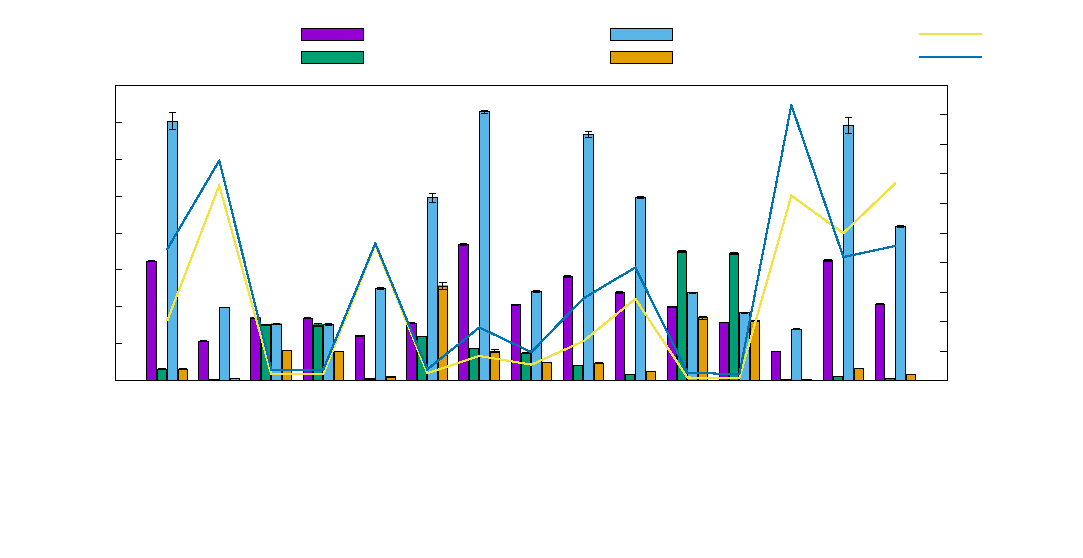
\includegraphics[width={504.00bp},height={252.00bp}]{all-hist-OnlineSetupTimesec}}%
    \gplfronttext
  \end{picture}%
\endgroup
}
% GNUPLOT: LaTeX picture with Postscript
\begingroup
  \makeatletter
  \providecommand\color[2][]{%
    \GenericError{(gnuplot) \space\space\space\@spaces}{%
      Package color not loaded in conjunction with
      terminal option `colourtext'%
    }{See the gnuplot documentation for explanation.%
    }{Either use 'blacktext' in gnuplot or load the package
      color.sty in LaTeX.}%
    \renewcommand\color[2][]{}%
  }%
  \providecommand\includegraphics[2][]{%
    \GenericError{(gnuplot) \space\space\space\@spaces}{%
      Package graphicx or graphics not loaded%
    }{See the gnuplot documentation for explanation.%
    }{The gnuplot epslatex terminal needs graphicx.sty or graphics.sty.}%
    \renewcommand\includegraphics[2][]{}%
  }%
  \providecommand\rotatebox[2]{#2}%
  \@ifundefined{ifGPcolor}{%
    \newif\ifGPcolor
    \GPcolortrue
  }{}%
  \@ifundefined{ifGPblacktext}{%
    \newif\ifGPblacktext
    \GPblacktextfalse
  }{}%
  % define a \g@addto@macro without @ in the name:
  \let\gplgaddtomacro\g@addto@macro
  % define empty templates for all commands taking text:
  \gdef\gplbacktext{}%
  \gdef\gplfronttext{}%
  \makeatother
  \ifGPblacktext
    % no textcolor at all
    \def\colorrgb#1{}%
    \def\colorgray#1{}%
  \else
    % gray or color?
    \ifGPcolor
      \def\colorrgb#1{\color[rgb]{#1}}%
      \def\colorgray#1{\color[gray]{#1}}%
      \expandafter\def\csname LTw\endcsname{\color{white}}%
      \expandafter\def\csname LTb\endcsname{\color{black}}%
      \expandafter\def\csname LTa\endcsname{\color{black}}%
      \expandafter\def\csname LT0\endcsname{\color[rgb]{1,0,0}}%
      \expandafter\def\csname LT1\endcsname{\color[rgb]{0,1,0}}%
      \expandafter\def\csname LT2\endcsname{\color[rgb]{0,0,1}}%
      \expandafter\def\csname LT3\endcsname{\color[rgb]{1,0,1}}%
      \expandafter\def\csname LT4\endcsname{\color[rgb]{0,1,1}}%
      \expandafter\def\csname LT5\endcsname{\color[rgb]{1,1,0}}%
      \expandafter\def\csname LT6\endcsname{\color[rgb]{0,0,0}}%
      \expandafter\def\csname LT7\endcsname{\color[rgb]{1,0.3,0}}%
      \expandafter\def\csname LT8\endcsname{\color[rgb]{0.5,0.5,0.5}}%
    \else
      % gray
      \def\colorrgb#1{\color{black}}%
      \def\colorgray#1{\color[gray]{#1}}%
      \expandafter\def\csname LTw\endcsname{\color{white}}%
      \expandafter\def\csname LTb\endcsname{\color{black}}%
      \expandafter\def\csname LTa\endcsname{\color{black}}%
      \expandafter\def\csname LT0\endcsname{\color{black}}%
      \expandafter\def\csname LT1\endcsname{\color{black}}%
      \expandafter\def\csname LT2\endcsname{\color{black}}%
      \expandafter\def\csname LT3\endcsname{\color{black}}%
      \expandafter\def\csname LT4\endcsname{\color{black}}%
      \expandafter\def\csname LT5\endcsname{\color{black}}%
      \expandafter\def\csname LT6\endcsname{\color{black}}%
      \expandafter\def\csname LT7\endcsname{\color{black}}%
      \expandafter\def\csname LT8\endcsname{\color{black}}%
    \fi
  \fi
    \setlength{\unitlength}{0.0500bp}%
    \ifx\gptboxheight\undefined%
      \newlength{\gptboxheight}%
      \newlength{\gptboxwidth}%
      \newsavebox{\gptboxtext}%
    \fi%
    \setlength{\fboxrule}{0.5pt}%
    \setlength{\fboxsep}{1pt}%
    \definecolor{tbcol}{rgb}{1,1,1}%
\begin{picture}(10080.00,5040.00)%
    \gplgaddtomacro\gplbacktext{%
      \csname LTb\endcsname%%
      \put(814,1100){\makebox(0,0)[r]{\strut{}$0$}}%
      \put(814,1510){\makebox(0,0)[r]{\strut{}$50$}}%
      \put(814,1920){\makebox(0,0)[r]{\strut{}$100$}}%
      \put(814,2330){\makebox(0,0)[r]{\strut{}$150$}}%
      \put(814,2740){\makebox(0,0)[r]{\strut{}$200$}}%
      \put(814,3149){\makebox(0,0)[r]{\strut{}$250$}}%
      \put(814,3559){\makebox(0,0)[r]{\strut{}$300$}}%
      \put(814,3969){\makebox(0,0)[r]{\strut{}$350$}}%
      \put(814,4379){\makebox(0,0)[r]{\strut{}$400$}}%
      \put(1416,968){\rotatebox{-45}{\makebox(0,0)[l]{\strut{}Biometric Matching}}}%
      \put(1886,968){\rotatebox{-45}{\makebox(0,0)[l]{\strut{}Biometric Matching (Fast)}}}%
      \put(2356,968){\rotatebox{-45}{\makebox(0,0)[l]{\strut{}Convex Hull}}}%
      \put(2826,968){\rotatebox{-45}{\makebox(0,0)[l]{\strut{}Count 102}}}%
      \put(3296,968){\rotatebox{-45}{\makebox(0,0)[l]{\strut{}Count 10s}}}%
      \put(3766,968){\rotatebox{-45}{\makebox(0,0)[l]{\strut{}Cryptonets (Max Pooling)}}}%
      \put(4236,968){\rotatebox{-45}{\makebox(0,0)[l]{\strut{}Database Join}}}%
      \put(4706,968){\rotatebox{-45}{\makebox(0,0)[l]{\strut{}Database Variance}}}%
      \put(5175,968){\rotatebox{-45}{\makebox(0,0)[l]{\strut{}Histogram}}}%
      \put(5645,968){\rotatebox{-45}{\makebox(0,0)[l]{\strut{}Inner Product}}}%
      \put(6115,968){\rotatebox{-45}{\makebox(0,0)[l]{\strut{}k-means}}}%
      \put(6585,968){\rotatebox{-45}{\makebox(0,0)[l]{\strut{}Longest 102}}}%
      \put(7055,968){\rotatebox{-45}{\makebox(0,0)[l]{\strut{}Max. Dist. b/w Symbols}}}%
      \put(7525,968){\rotatebox{-45}{\makebox(0,0)[l]{\strut{}Minimal Points}}}%
      \put(7995,968){\rotatebox{-45}{\makebox(0,0)[l]{\strut{}MNIST ReLU}}}%
      \put(8465,968){\rotatebox{-45}{\makebox(0,0)[l]{\strut{}Private Set Intersection}}}%
      \put(9067,1100){\makebox(0,0)[l]{\strut{}$0$}}%
      \put(9067,1568){\makebox(0,0)[l]{\strut{}$10$}}%
      \put(9067,2037){\makebox(0,0)[l]{\strut{}$20$}}%
      \put(9067,2505){\makebox(0,0)[l]{\strut{}$30$}}%
      \put(9067,2974){\makebox(0,0)[l]{\strut{}$40$}}%
      \put(9067,3442){\makebox(0,0)[l]{\strut{}$50$}}%
      \put(9067,3911){\makebox(0,0)[l]{\strut{}$60$}}%
      \put(9067,4379){\makebox(0,0)[l]{\strut{}$70$}}%
    }%
    \gplgaddtomacro\gplfronttext{%
      \csname LTb\endcsname%%
      \put(209,2739){\rotatebox{-270}{\makebox(0,0){\strut{}Online + Setup Time (sec)}}}%
      \put(9573,2739){\rotatebox{-270}{\makebox(0,0){\strut{}Improvement (number of times)}}}%
      \csname LTb\endcsname%%
      \put(2602,4867){\makebox(0,0)[r]{\strut{}GMW}}%
      \csname LTb\endcsname%%
      \put(2602,4647){\makebox(0,0)[r]{\strut{}GMW (Vectorized)}}%
      \csname LTb\endcsname%%
      \put(5569,4867){\makebox(0,0)[r]{\strut{}BMR}}%
      \csname LTb\endcsname%%
      \put(5569,4647){\makebox(0,0)[r]{\strut{}BMR (Vectorized)}}%
      \csname LTb\endcsname%%
      \put(8536,4867){\makebox(0,0)[r]{\strut{}GMW Improvement}}%
      \csname LTb\endcsname%%
      \put(8536,4647){\makebox(0,0)[r]{\strut{}BMR Improvement}}%
    }%
    \gplbacktext
    \put(0,0){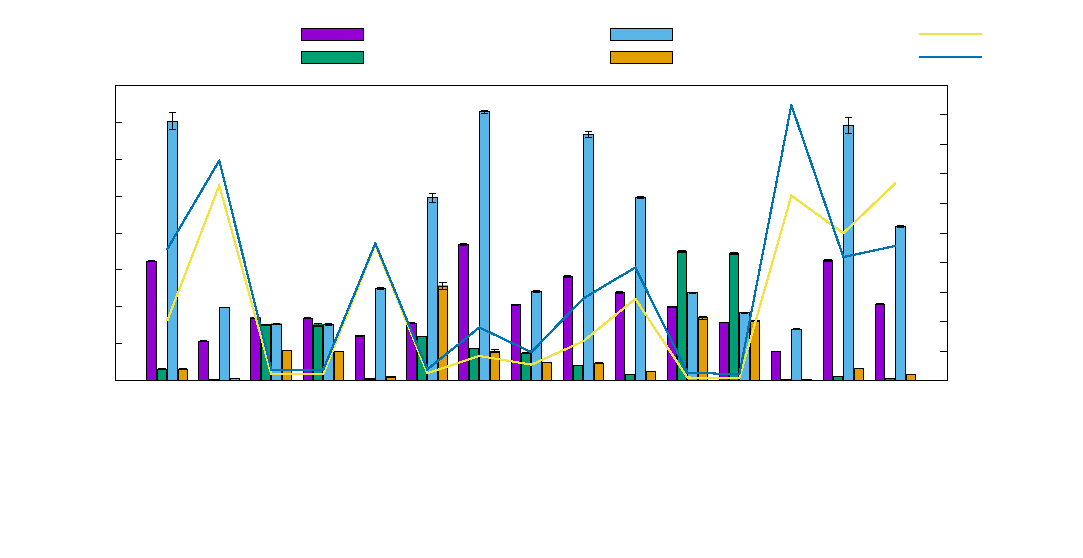
\includegraphics[width={504.00bp},height={252.00bp}]{all-hist-OnlineSetupTimesec}}%
    \gplfronttext
  \end{picture}%
\endgroup

\caption{Circuit Evaluation Time (Setup + Online) of Benchmarks}
\label{fig:graph_all_eval_time}
\end{figure*}

A detailed summery of the effects of vectorization on various benchmarks is presented in \cref{table:metrics}. We show circuit evaluation times in \cref{fig:graph_all_eval_time}. In terms of amenability to vectorization, we divide benchmarks into 3 categories: 1) {\it High:} these include convex hull, cryptonets max pooling, minimal points and private set intersection. These benchmarks are highly parallelizable and see 25x to 70x speedup in BMR, and 30x to 55x in GMW protocol. 2) {\it Medium:} these include biometric matching, DB Variance, histogram, inner product, k-means iteration and MNIST ReLU. These benchmarks have non-parallelizable phases e.g. the summing phase of inner product and biometric matching. Still, most computation is parallelizable and it results in speedup from 5x to 25x in BMR, and 2x to 25x in GMW protocol. 3) {\it Low:} these include the Database Join and the regular expression benchmarks (count 102, count 10, longest 102 and max distance between symbols). There is very little parallelizable computation in these programs, thus the speedup is lower. We see a speedup from 1.1x to 2x in BMR. In GMW, DB Join, Count 102 and Count 10s see speedup from 1.1x to 1.3x. However, longest 102 and max distance between symbols suffer a slowdown of 0.5x. The structure of these benchmarks is such that transformation to vectorized code increases multiplicative depth and, the negative effect of increased depth is more noticeable in a round-based protocol like GMW. We fix this via a simple heuristic where if the transformation increases circuit depth beyond some threshold (e.g. more than 10\% of the original circuit), we reject the transformation. Nevertheless, we show these graphs here for the sake of completeness and to highlight that vectorization is not always reduce run time. Note that in some settings it may still be desirable to vectorize e.g. in data constrained environments. As shown in \cref{fig:graph_comm_size}, vectorization results in reduced communication (fewer bits are transferred).

We present evaluation for communication size in \cref{fig:graph_comm_size_time}, circuit generation time in \cref{fig:graph_circ_gen_time}, number of gates in \cref{fig:graph_total_gates} and online time and setup time in \cref{fig:graph_online_time} and \cref{fig:graph_setup_time} respectively. \ishaq{Ana: Let me know if I should add more substance.}


\begin{figure}[htbp]
\centering
\resizebox{3.6in}{!}{\input{graphs/lan/biometric-hist-OnlineSetupTimesec}}
\caption{Biometric Matching Circuit Evaluation Time, x-axis lists database size}
\label{fig:graph_biometric_eval_time}
\end{figure}

\begin{figure}[htbp]
\centering
\resizebox{3.6in}{!}{% GNUPLOT: LaTeX picture with Postscript
\begingroup
  \makeatletter
  \providecommand\color[2][]{%
    \GenericError{(gnuplot) \space\space\space\@spaces}{%
      Package color not loaded in conjunction with
      terminal option `colourtext'%
    }{See the gnuplot documentation for explanation.%
    }{Either use 'blacktext' in gnuplot or load the package
      color.sty in LaTeX.}%
    \renewcommand\color[2][]{}%
  }%
  \providecommand\includegraphics[2][]{%
    \GenericError{(gnuplot) \space\space\space\@spaces}{%
      Package graphicx or graphics not loaded%
    }{See the gnuplot documentation for explanation.%
    }{The gnuplot epslatex terminal needs graphicx.sty or graphics.sty.}%
    \renewcommand\includegraphics[2][]{}%
  }%
  \providecommand\rotatebox[2]{#2}%
  \@ifundefined{ifGPcolor}{%
    \newif\ifGPcolor
    \GPcolortrue
  }{}%
  \@ifundefined{ifGPblacktext}{%
    \newif\ifGPblacktext
    \GPblacktextfalse
  }{}%
  % define a \g@addto@macro without @ in the name:
  \let\gplgaddtomacro\g@addto@macro
  % define empty templates for all commands taking text:
  \gdef\gplbacktext{}%
  \gdef\gplfronttext{}%
  \makeatother
  \ifGPblacktext
    % no textcolor at all
    \def\colorrgb#1{}%
    \def\colorgray#1{}%
  \else
    % gray or color?
    \ifGPcolor
      \def\colorrgb#1{\color[rgb]{#1}}%
      \def\colorgray#1{\color[gray]{#1}}%
      \expandafter\def\csname LTw\endcsname{\color{white}}%
      \expandafter\def\csname LTb\endcsname{\color{black}}%
      \expandafter\def\csname LTa\endcsname{\color{black}}%
      \expandafter\def\csname LT0\endcsname{\color[rgb]{1,0,0}}%
      \expandafter\def\csname LT1\endcsname{\color[rgb]{0,1,0}}%
      \expandafter\def\csname LT2\endcsname{\color[rgb]{0,0,1}}%
      \expandafter\def\csname LT3\endcsname{\color[rgb]{1,0,1}}%
      \expandafter\def\csname LT4\endcsname{\color[rgb]{0,1,1}}%
      \expandafter\def\csname LT5\endcsname{\color[rgb]{1,1,0}}%
      \expandafter\def\csname LT6\endcsname{\color[rgb]{0,0,0}}%
      \expandafter\def\csname LT7\endcsname{\color[rgb]{1,0.3,0}}%
      \expandafter\def\csname LT8\endcsname{\color[rgb]{0.5,0.5,0.5}}%
    \else
      % gray
      \def\colorrgb#1{\color{black}}%
      \def\colorgray#1{\color[gray]{#1}}%
      \expandafter\def\csname LTw\endcsname{\color{white}}%
      \expandafter\def\csname LTb\endcsname{\color{black}}%
      \expandafter\def\csname LTa\endcsname{\color{black}}%
      \expandafter\def\csname LT0\endcsname{\color{black}}%
      \expandafter\def\csname LT1\endcsname{\color{black}}%
      \expandafter\def\csname LT2\endcsname{\color{black}}%
      \expandafter\def\csname LT3\endcsname{\color{black}}%
      \expandafter\def\csname LT4\endcsname{\color{black}}%
      \expandafter\def\csname LT5\endcsname{\color{black}}%
      \expandafter\def\csname LT6\endcsname{\color{black}}%
      \expandafter\def\csname LT7\endcsname{\color{black}}%
      \expandafter\def\csname LT8\endcsname{\color{black}}%
    \fi
  \fi
    \setlength{\unitlength}{0.0500bp}%
    \ifx\gptboxheight\undefined%
      \newlength{\gptboxheight}%
      \newlength{\gptboxwidth}%
      \newsavebox{\gptboxtext}%
    \fi%
    \setlength{\fboxrule}{0.5pt}%
    \setlength{\fboxsep}{1pt}%
    \definecolor{tbcol}{rgb}{1,1,1}%
\begin{picture}(5760.00,4320.00)%
    \gplgaddtomacro\gplbacktext{%
      \csname LTb\endcsname%%
      \put(946,440){\makebox(0,0)[r]{\strut{}$0$}}%
      \put(946,847){\makebox(0,0)[r]{\strut{}$500$}}%
      \put(946,1253){\makebox(0,0)[r]{\strut{}$1000$}}%
      \put(946,1660){\makebox(0,0)[r]{\strut{}$1500$}}%
      \put(946,2066){\makebox(0,0)[r]{\strut{}$2000$}}%
      \put(946,2473){\makebox(0,0)[r]{\strut{}$2500$}}%
      \put(946,2879){\makebox(0,0)[r]{\strut{}$3000$}}%
      \put(946,3286){\makebox(0,0)[r]{\strut{}$3500$}}%
      \put(946,3692){\makebox(0,0)[r]{\strut{}$4000$}}%
      \put(946,4099){\makebox(0,0)[r]{\strut{}$4500$}}%
      \put(1373,308){\rotatebox{-45}{\makebox(0,0)[l]{\strut{}N: 4}}}%
      \put(1668,308){\rotatebox{-45}{\makebox(0,0)[l]{\strut{}N: 8}}}%
      \put(1962,308){\rotatebox{-45}{\makebox(0,0)[l]{\strut{}N: 16}}}%
      \put(2257,308){\rotatebox{-45}{\makebox(0,0)[l]{\strut{}N: 32}}}%
      \put(2552,308){\rotatebox{-45}{\makebox(0,0)[l]{\strut{}N: 64}}}%
      \put(2847,308){\rotatebox{-45}{\makebox(0,0)[l]{\strut{}N: 128}}}%
      \put(3141,308){\rotatebox{-45}{\makebox(0,0)[l]{\strut{}N: 256}}}%
      \put(3436,308){\rotatebox{-45}{\makebox(0,0)[l]{\strut{}N: 512}}}%
      \put(3731,308){\rotatebox{-45}{\makebox(0,0)[l]{\strut{}N: 1024}}}%
      \put(4026,308){\rotatebox{-45}{\makebox(0,0)[l]{\strut{}N: 2048}}}%
      \put(4320,308){\rotatebox{-45}{\makebox(0,0)[l]{\strut{}N: 4096}}}%
      \put(4747,440){\makebox(0,0)[l]{\strut{}$0$}}%
      \put(4747,1050){\makebox(0,0)[l]{\strut{}$2$}}%
      \put(4747,1660){\makebox(0,0)[l]{\strut{}$4$}}%
      \put(4747,2270){\makebox(0,0)[l]{\strut{}$6$}}%
      \put(4747,2879){\makebox(0,0)[l]{\strut{}$8$}}%
      \put(4747,3489){\makebox(0,0)[l]{\strut{}$10$}}%
      \put(4747,4099){\makebox(0,0)[l]{\strut{}$12$}}%
    }%
    \gplgaddtomacro\gplfronttext{%
      \csname LTb\endcsname%%
      \put(209,2269){\rotatebox{-270}{\makebox(0,0){\strut{}Communication (MiB)}}}%
      \put(5253,2269){\rotatebox{-270}{\makebox(0,0){\strut{}Improvement (number of times)}}}%
      \csname LTb\endcsname%%
      \put(3322,3926){\makebox(0,0)[r]{\strut{}GMW}}%
      \csname LTb\endcsname%%
      \put(3322,3706){\makebox(0,0)[r]{\strut{}GMW (Vectorized)}}%
      \csname LTb\endcsname%%
      \put(3322,3486){\makebox(0,0)[r]{\strut{}BMR}}%
      \csname LTb\endcsname%%
      \put(3322,3266){\makebox(0,0)[r]{\strut{}BMR (Vectorized)}}%
      \csname LTb\endcsname%%
      \put(3322,3046){\makebox(0,0)[r]{\strut{}GMW Improvement}}%
      \csname LTb\endcsname%%
      \put(3322,2826){\makebox(0,0)[r]{\strut{}BMR Improvement}}%
    }%
    \gplbacktext
    \put(0,0){\includegraphics[width={288.00bp},height={216.00bp}]{biometric-hist-CommunicationMiB}}%
    \gplfronttext
  \end{picture}%
\endgroup
}
\caption{Biometric Matching Communication Size, x-axis lists database size}
\label{fig:graph_biometic_comm_size}
\end{figure}

\begin{figure}[htbp]
\centering
\resizebox{3.6in}{!}{% GNUPLOT: LaTeX picture with Postscript
\begingroup
  \makeatletter
  \providecommand\color[2][]{%
    \GenericError{(gnuplot) \space\space\space\@spaces}{%
      Package color not loaded in conjunction with
      terminal option `colourtext'%
    }{See the gnuplot documentation for explanation.%
    }{Either use 'blacktext' in gnuplot or load the package
      color.sty in LaTeX.}%
    \renewcommand\color[2][]{}%
  }%
  \providecommand\includegraphics[2][]{%
    \GenericError{(gnuplot) \space\space\space\@spaces}{%
      Package graphicx or graphics not loaded%
    }{See the gnuplot documentation for explanation.%
    }{The gnuplot epslatex terminal needs graphicx.sty or graphics.sty.}%
    \renewcommand\includegraphics[2][]{}%
  }%
  \providecommand\rotatebox[2]{#2}%
  \@ifundefined{ifGPcolor}{%
    \newif\ifGPcolor
    \GPcolortrue
  }{}%
  \@ifundefined{ifGPblacktext}{%
    \newif\ifGPblacktext
    \GPblacktextfalse
  }{}%
  % define a \g@addto@macro without @ in the name:
  \let\gplgaddtomacro\g@addto@macro
  % define empty templates for all commands taking text:
  \gdef\gplbacktext{}%
  \gdef\gplfronttext{}%
  \makeatother
  \ifGPblacktext
    % no textcolor at all
    \def\colorrgb#1{}%
    \def\colorgray#1{}%
  \else
    % gray or color?
    \ifGPcolor
      \def\colorrgb#1{\color[rgb]{#1}}%
      \def\colorgray#1{\color[gray]{#1}}%
      \expandafter\def\csname LTw\endcsname{\color{white}}%
      \expandafter\def\csname LTb\endcsname{\color{black}}%
      \expandafter\def\csname LTa\endcsname{\color{black}}%
      \expandafter\def\csname LT0\endcsname{\color[rgb]{1,0,0}}%
      \expandafter\def\csname LT1\endcsname{\color[rgb]{0,1,0}}%
      \expandafter\def\csname LT2\endcsname{\color[rgb]{0,0,1}}%
      \expandafter\def\csname LT3\endcsname{\color[rgb]{1,0,1}}%
      \expandafter\def\csname LT4\endcsname{\color[rgb]{0,1,1}}%
      \expandafter\def\csname LT5\endcsname{\color[rgb]{1,1,0}}%
      \expandafter\def\csname LT6\endcsname{\color[rgb]{0,0,0}}%
      \expandafter\def\csname LT7\endcsname{\color[rgb]{1,0.3,0}}%
      \expandafter\def\csname LT8\endcsname{\color[rgb]{0.5,0.5,0.5}}%
    \else
      % gray
      \def\colorrgb#1{\color{black}}%
      \def\colorgray#1{\color[gray]{#1}}%
      \expandafter\def\csname LTw\endcsname{\color{white}}%
      \expandafter\def\csname LTb\endcsname{\color{black}}%
      \expandafter\def\csname LTa\endcsname{\color{black}}%
      \expandafter\def\csname LT0\endcsname{\color{black}}%
      \expandafter\def\csname LT1\endcsname{\color{black}}%
      \expandafter\def\csname LT2\endcsname{\color{black}}%
      \expandafter\def\csname LT3\endcsname{\color{black}}%
      \expandafter\def\csname LT4\endcsname{\color{black}}%
      \expandafter\def\csname LT5\endcsname{\color{black}}%
      \expandafter\def\csname LT6\endcsname{\color{black}}%
      \expandafter\def\csname LT7\endcsname{\color{black}}%
      \expandafter\def\csname LT8\endcsname{\color{black}}%
    \fi
  \fi
    \setlength{\unitlength}{0.0500bp}%
    \ifx\gptboxheight\undefined%
      \newlength{\gptboxheight}%
      \newlength{\gptboxwidth}%
      \newsavebox{\gptboxtext}%
    \fi%
    \setlength{\fboxrule}{0.5pt}%
    \setlength{\fboxsep}{1pt}%
    \definecolor{tbcol}{rgb}{1,1,1}%
\begin{picture}(5760.00,4320.00)%
    \gplgaddtomacro\gplbacktext{%
      \csname LTb\endcsname%%
      \put(814,440){\makebox(0,0)[r]{\strut{}$0$}}%
      \put(814,963){\makebox(0,0)[r]{\strut{}$20$}}%
      \put(814,1485){\makebox(0,0)[r]{\strut{}$40$}}%
      \put(814,2008){\makebox(0,0)[r]{\strut{}$60$}}%
      \put(814,2531){\makebox(0,0)[r]{\strut{}$80$}}%
      \put(814,3054){\makebox(0,0)[r]{\strut{}$100$}}%
      \put(814,3576){\makebox(0,0)[r]{\strut{}$120$}}%
      \put(814,4099){\makebox(0,0)[r]{\strut{}$140$}}%
      \put(1252,308){\rotatebox{-45}{\makebox(0,0)[l]{\strut{}N: 4}}}%
      \put(1558,308){\rotatebox{-45}{\makebox(0,0)[l]{\strut{}N: 8}}}%
      \put(1863,308){\rotatebox{-45}{\makebox(0,0)[l]{\strut{}N: 16}}}%
      \put(2169,308){\rotatebox{-45}{\makebox(0,0)[l]{\strut{}N: 32}}}%
      \put(2475,308){\rotatebox{-45}{\makebox(0,0)[l]{\strut{}N: 64}}}%
      \put(2781,308){\rotatebox{-45}{\makebox(0,0)[l]{\strut{}N: 128}}}%
      \put(3086,308){\rotatebox{-45}{\makebox(0,0)[l]{\strut{}N: 256}}}%
      \put(3392,308){\rotatebox{-45}{\makebox(0,0)[l]{\strut{}N: 512}}}%
      \put(3698,308){\rotatebox{-45}{\makebox(0,0)[l]{\strut{}N: 1024}}}%
      \put(4004,308){\rotatebox{-45}{\makebox(0,0)[l]{\strut{}N: 2048}}}%
      \put(4309,308){\rotatebox{-45}{\makebox(0,0)[l]{\strut{}N: 4096}}}%
      \put(4747,440){\makebox(0,0)[l]{\strut{}$0$}}%
      \put(4747,806){\makebox(0,0)[l]{\strut{}$5$}}%
      \put(4747,1172){\makebox(0,0)[l]{\strut{}$10$}}%
      \put(4747,1538){\makebox(0,0)[l]{\strut{}$15$}}%
      \put(4747,1904){\makebox(0,0)[l]{\strut{}$20$}}%
      \put(4747,2270){\makebox(0,0)[l]{\strut{}$25$}}%
      \put(4747,2635){\makebox(0,0)[l]{\strut{}$30$}}%
      \put(4747,3001){\makebox(0,0)[l]{\strut{}$35$}}%
      \put(4747,3367){\makebox(0,0)[l]{\strut{}$40$}}%
      \put(4747,3733){\makebox(0,0)[l]{\strut{}$45$}}%
      \put(4747,4099){\makebox(0,0)[l]{\strut{}$50$}}%
    }%
    \gplgaddtomacro\gplfronttext{%
      \csname LTb\endcsname%%
      \put(209,2269){\rotatebox{-270}{\makebox(0,0){\strut{}Circuit Generation Time (sec)}}}%
      \put(5253,2269){\rotatebox{-270}{\makebox(0,0){\strut{}Improvement (number of times)}}}%
      \csname LTb\endcsname%%
      \put(3190,3926){\makebox(0,0)[r]{\strut{}GMW}}%
      \csname LTb\endcsname%%
      \put(3190,3706){\makebox(0,0)[r]{\strut{}GMW (Vectorized)}}%
      \csname LTb\endcsname%%
      \put(3190,3486){\makebox(0,0)[r]{\strut{}BMR}}%
      \csname LTb\endcsname%%
      \put(3190,3266){\makebox(0,0)[r]{\strut{}BMR (Vectorized)}}%
      \csname LTb\endcsname%%
      \put(3190,3046){\makebox(0,0)[r]{\strut{}GMW Improvement}}%
      \csname LTb\endcsname%%
      \put(3190,2826){\makebox(0,0)[r]{\strut{}BMR Improvement}}%
    }%
    \gplbacktext
    \put(0,0){\includegraphics[width={288.00bp},height={216.00bp}]{biometric-hist-CircuitGenerationTimesec}}%
    \gplfronttext
  \end{picture}%
\endgroup
}
\caption{Biometric Matching Circuit Generation Time, x-axis lists database size}
\label{fig:graph_biometic_circ_gen_time}
\end{figure}

Next, we look closely at circuit evaluation \cref{fig:graph_biometric_eval_time}, communication size \cref{fig:graph_biometic_comm_size} and circuit generation time \cref{fig:graph_biometic_circ_gen_time} for biometric matching benchmark. For input size beyond {\tt N=128} the memory usage exceeds available memory and prevents circuit generation. Consequently, non-vectorized bars are missing beyond this threshold. Notice that vectorization improves all metrics. A database of size {\tt N=128} is smaller than any real world usecase, therefore lets use it as baseline for improvement. Comparing performance improvement between BMR and GMW, we see more speedup for BMR (23x vs 10x), GMW gets more communication size reduction (10x vs 2.5x) and circuit generation sees a speedup of 35x and 45x for BMR and GMW respectively. 



\begin{figure}[htbp]
\centering
\resizebox{3.6in}{!}{% GNUPLOT: LaTeX picture with Postscript
\begingroup
  \makeatletter
  \providecommand\color[2][]{%
    \GenericError{(gnuplot) \space\space\space\@spaces}{%
      Package color not loaded in conjunction with
      terminal option `colourtext'%
    }{See the gnuplot documentation for explanation.%
    }{Either use 'blacktext' in gnuplot or load the package
      color.sty in LaTeX.}%
    \renewcommand\color[2][]{}%
  }%
  \providecommand\includegraphics[2][]{%
    \GenericError{(gnuplot) \space\space\space\@spaces}{%
      Package graphicx or graphics not loaded%
    }{See the gnuplot documentation for explanation.%
    }{The gnuplot epslatex terminal needs graphicx.sty or graphics.sty.}%
    \renewcommand\includegraphics[2][]{}%
  }%
  \providecommand\rotatebox[2]{#2}%
  \@ifundefined{ifGPcolor}{%
    \newif\ifGPcolor
    \GPcolortrue
  }{}%
  \@ifundefined{ifGPblacktext}{%
    \newif\ifGPblacktext
    \GPblacktextfalse
  }{}%
  % define a \g@addto@macro without @ in the name:
  \let\gplgaddtomacro\g@addto@macro
  % define empty templates for all commands taking text:
  \gdef\gplbacktext{}%
  \gdef\gplfronttext{}%
  \makeatother
  \ifGPblacktext
    % no textcolor at all
    \def\colorrgb#1{}%
    \def\colorgray#1{}%
  \else
    % gray or color?
    \ifGPcolor
      \def\colorrgb#1{\color[rgb]{#1}}%
      \def\colorgray#1{\color[gray]{#1}}%
      \expandafter\def\csname LTw\endcsname{\color{white}}%
      \expandafter\def\csname LTb\endcsname{\color{black}}%
      \expandafter\def\csname LTa\endcsname{\color{black}}%
      \expandafter\def\csname LT0\endcsname{\color[rgb]{1,0,0}}%
      \expandafter\def\csname LT1\endcsname{\color[rgb]{0,1,0}}%
      \expandafter\def\csname LT2\endcsname{\color[rgb]{0,0,1}}%
      \expandafter\def\csname LT3\endcsname{\color[rgb]{1,0,1}}%
      \expandafter\def\csname LT4\endcsname{\color[rgb]{0,1,1}}%
      \expandafter\def\csname LT5\endcsname{\color[rgb]{1,1,0}}%
      \expandafter\def\csname LT6\endcsname{\color[rgb]{0,0,0}}%
      \expandafter\def\csname LT7\endcsname{\color[rgb]{1,0.3,0}}%
      \expandafter\def\csname LT8\endcsname{\color[rgb]{0.5,0.5,0.5}}%
    \else
      % gray
      \def\colorrgb#1{\color{black}}%
      \def\colorgray#1{\color[gray]{#1}}%
      \expandafter\def\csname LTw\endcsname{\color{white}}%
      \expandafter\def\csname LTb\endcsname{\color{black}}%
      \expandafter\def\csname LTa\endcsname{\color{black}}%
      \expandafter\def\csname LT0\endcsname{\color{black}}%
      \expandafter\def\csname LT1\endcsname{\color{black}}%
      \expandafter\def\csname LT2\endcsname{\color{black}}%
      \expandafter\def\csname LT3\endcsname{\color{black}}%
      \expandafter\def\csname LT4\endcsname{\color{black}}%
      \expandafter\def\csname LT5\endcsname{\color{black}}%
      \expandafter\def\csname LT6\endcsname{\color{black}}%
      \expandafter\def\csname LT7\endcsname{\color{black}}%
      \expandafter\def\csname LT8\endcsname{\color{black}}%
    \fi
  \fi
    \setlength{\unitlength}{0.0500bp}%
    \ifx\gptboxheight\undefined%
      \newlength{\gptboxheight}%
      \newlength{\gptboxwidth}%
      \newsavebox{\gptboxtext}%
    \fi%
    \setlength{\fboxrule}{0.5pt}%
    \setlength{\fboxsep}{1pt}%
    \definecolor{tbcol}{rgb}{1,1,1}%
\begin{picture}(5760.00,4320.00)%
    \gplgaddtomacro\gplbacktext{%
      \csname LTb\endcsname%%
      \put(946,660){\makebox(0,0)[r]{\strut{}$0$}}%
      \csname LTb\endcsname%%
      \put(946,1151){\makebox(0,0)[r]{\strut{}$500$}}%
      \csname LTb\endcsname%%
      \put(946,1643){\makebox(0,0)[r]{\strut{}$1000$}}%
      \csname LTb\endcsname%%
      \put(946,2134){\makebox(0,0)[r]{\strut{}$1500$}}%
      \csname LTb\endcsname%%
      \put(946,2625){\makebox(0,0)[r]{\strut{}$2000$}}%
      \csname LTb\endcsname%%
      \put(946,3116){\makebox(0,0)[r]{\strut{}$2500$}}%
      \csname LTb\endcsname%%
      \put(946,3608){\makebox(0,0)[r]{\strut{}$3000$}}%
      \csname LTb\endcsname%%
      \put(946,4099){\makebox(0,0)[r]{\strut{}$3500$}}%
      \csname LTb\endcsname%%
      \put(2149,528){\rotatebox{-25}{\makebox(0,0)[l]{\strut{}Biometric Matching}}}%
      \csname LTb\endcsname%%
      \put(3221,528){\rotatebox{-25}{\makebox(0,0)[l]{\strut{}Inner Product}}}%
      \csname LTb\endcsname%%
      \put(4292,528){\rotatebox{-25}{\makebox(0,0)[l]{\strut{}Longest 102}}}%
    }%
    \gplgaddtomacro\gplfronttext{%
      \csname LTb\endcsname%%
      \put(209,2379){\rotatebox{-270}{\makebox(0,0){\strut{}Online + Setup Time (sec)}}}%
      \csname LTb\endcsname%%
      \put(2134,3926){\makebox(0,0)[r]{\strut{}GMW LAN}}%
      \csname LTb\endcsname%%
      \put(2134,3706){\makebox(0,0)[r]{\strut{}GMW WAN}}%
      \csname LTb\endcsname%%
      \put(2134,3486){\makebox(0,0)[r]{\strut{}BMR LAN}}%
      \csname LTb\endcsname%%
      \put(2134,3266){\makebox(0,0)[r]{\strut{}BMR WAN}}%
    }%
    \gplbacktext
    \put(0,0){\includegraphics[width={288.00bp},height={216.00bp}]{comparison-hist-OnlineSetupTimesec}}%
    \gplfronttext
  \end{picture}%
\endgroup
}
\caption{LAN vs. WAN: Circuit Evaluation Time Comparison}
\label{fig:graph_comparison_eval_time}
\end{figure}

Since our vectorization framework is network agnostic, it produces the same circuit for both LAN and WAN. This means that the number of gates and communication size remain the same. Moreover, time for circuit generation, which is a local operation, also remains unchanged. Setup and Online times, however, increase due to lower bandwidth and higher latency of the WAN. Indeed, this is what we observe in \cref{fig:graph_comparison_eval_time}.

\begin{figure*}[htbp]
\centering
% GNUPLOT: LaTeX picture with Postscript
\begingroup
  \makeatletter
  \providecommand\color[2][]{%
    \GenericError{(gnuplot) \space\space\space\@spaces}{%
      Package color not loaded in conjunction with
      terminal option `colourtext'%
    }{See the gnuplot documentation for explanation.%
    }{Either use 'blacktext' in gnuplot or load the package
      color.sty in LaTeX.}%
    \renewcommand\color[2][]{}%
  }%
  \providecommand\includegraphics[2][]{%
    \GenericError{(gnuplot) \space\space\space\@spaces}{%
      Package graphicx or graphics not loaded%
    }{See the gnuplot documentation for explanation.%
    }{The gnuplot epslatex terminal needs graphicx.sty or graphics.sty.}%
    \renewcommand\includegraphics[2][]{}%
  }%
  \providecommand\rotatebox[2]{#2}%
  \@ifundefined{ifGPcolor}{%
    \newif\ifGPcolor
    \GPcolortrue
  }{}%
  \@ifundefined{ifGPblacktext}{%
    \newif\ifGPblacktext
    \GPblacktextfalse
  }{}%
  % define a \g@addto@macro without @ in the name:
  \let\gplgaddtomacro\g@addto@macro
  % define empty templates for all commands taking text:
  \gdef\gplbacktext{}%
  \gdef\gplfronttext{}%
  \makeatother
  \ifGPblacktext
    % no textcolor at all
    \def\colorrgb#1{}%
    \def\colorgray#1{}%
  \else
    % gray or color?
    \ifGPcolor
      \def\colorrgb#1{\color[rgb]{#1}}%
      \def\colorgray#1{\color[gray]{#1}}%
      \expandafter\def\csname LTw\endcsname{\color{white}}%
      \expandafter\def\csname LTb\endcsname{\color{black}}%
      \expandafter\def\csname LTa\endcsname{\color{black}}%
      \expandafter\def\csname LT0\endcsname{\color[rgb]{1,0,0}}%
      \expandafter\def\csname LT1\endcsname{\color[rgb]{0,1,0}}%
      \expandafter\def\csname LT2\endcsname{\color[rgb]{0,0,1}}%
      \expandafter\def\csname LT3\endcsname{\color[rgb]{1,0,1}}%
      \expandafter\def\csname LT4\endcsname{\color[rgb]{0,1,1}}%
      \expandafter\def\csname LT5\endcsname{\color[rgb]{1,1,0}}%
      \expandafter\def\csname LT6\endcsname{\color[rgb]{0,0,0}}%
      \expandafter\def\csname LT7\endcsname{\color[rgb]{1,0.3,0}}%
      \expandafter\def\csname LT8\endcsname{\color[rgb]{0.5,0.5,0.5}}%
    \else
      % gray
      \def\colorrgb#1{\color{black}}%
      \def\colorgray#1{\color[gray]{#1}}%
      \expandafter\def\csname LTw\endcsname{\color{white}}%
      \expandafter\def\csname LTb\endcsname{\color{black}}%
      \expandafter\def\csname LTa\endcsname{\color{black}}%
      \expandafter\def\csname LT0\endcsname{\color{black}}%
      \expandafter\def\csname LT1\endcsname{\color{black}}%
      \expandafter\def\csname LT2\endcsname{\color{black}}%
      \expandafter\def\csname LT3\endcsname{\color{black}}%
      \expandafter\def\csname LT4\endcsname{\color{black}}%
      \expandafter\def\csname LT5\endcsname{\color{black}}%
      \expandafter\def\csname LT6\endcsname{\color{black}}%
      \expandafter\def\csname LT7\endcsname{\color{black}}%
      \expandafter\def\csname LT8\endcsname{\color{black}}%
    \fi
  \fi
    \setlength{\unitlength}{0.0500bp}%
    \ifx\gptboxheight\undefined%
      \newlength{\gptboxheight}%
      \newlength{\gptboxwidth}%
      \newsavebox{\gptboxtext}%
    \fi%
    \setlength{\fboxrule}{0.5pt}%
    \setlength{\fboxsep}{1pt}%
    \definecolor{tbcol}{rgb}{1,1,1}%
\begin{picture}(10080.00,5040.00)%
    \gplgaddtomacro\gplbacktext{%
      \csname LTb\endcsname%%
      \put(814,1540){\makebox(0,0)[r]{\strut{}$0$}}%
      \put(814,1855){\makebox(0,0)[r]{\strut{}$50$}}%
      \put(814,2171){\makebox(0,0)[r]{\strut{}$100$}}%
      \put(814,2486){\makebox(0,0)[r]{\strut{}$150$}}%
      \put(814,2802){\makebox(0,0)[r]{\strut{}$200$}}%
      \put(814,3117){\makebox(0,0)[r]{\strut{}$250$}}%
      \put(814,3433){\makebox(0,0)[r]{\strut{}$300$}}%
      \put(814,3748){\makebox(0,0)[r]{\strut{}$350$}}%
      \put(814,4064){\makebox(0,0)[r]{\strut{}$400$}}%
      \put(814,4379){\makebox(0,0)[r]{\strut{}$450$}}%
      \put(1416,1408){\rotatebox{-45}{\makebox(0,0)[l]{\strut{}Biometric Matching}}}%
      \put(1886,1408){\rotatebox{-45}{\makebox(0,0)[l]{\strut{}Biometric Matching (Fast)}}}%
      \put(2356,1408){\rotatebox{-45}{\makebox(0,0)[l]{\strut{}Convex Hull}}}%
      \put(2826,1408){\rotatebox{-45}{\makebox(0,0)[l]{\strut{}Count 102}}}%
      \put(3296,1408){\rotatebox{-45}{\makebox(0,0)[l]{\strut{}Count 10s}}}%
      \put(3766,1408){\rotatebox{-45}{\makebox(0,0)[l]{\strut{}Cryptonets (Max Pooling)}}}%
      \put(4236,1408){\rotatebox{-45}{\makebox(0,0)[l]{\strut{}Database Join}}}%
      \put(4706,1408){\rotatebox{-45}{\makebox(0,0)[l]{\strut{}Database Variance}}}%
      \put(5175,1408){\rotatebox{-45}{\makebox(0,0)[l]{\strut{}Histogram}}}%
      \put(5645,1408){\rotatebox{-45}{\makebox(0,0)[l]{\strut{}Inner Product}}}%
      \put(6115,1408){\rotatebox{-45}{\makebox(0,0)[l]{\strut{}k-means}}}%
      \put(6585,1408){\rotatebox{-45}{\makebox(0,0)[l]{\strut{}Longest 102}}}%
      \put(7055,1408){\rotatebox{-45}{\makebox(0,0)[l]{\strut{}Max. Dist. b/w Symbols}}}%
      \put(7525,1408){\rotatebox{-45}{\makebox(0,0)[l]{\strut{}Minimal Points}}}%
      \put(7995,1408){\rotatebox{-45}{\makebox(0,0)[l]{\strut{}MNIST ReLU}}}%
      \put(8465,1408){\rotatebox{-45}{\makebox(0,0)[l]{\strut{}Private Set Intersection}}}%
      \put(9067,1540){\makebox(0,0)[l]{\strut{}$0$}}%
      \put(9067,1946){\makebox(0,0)[l]{\strut{}$2$}}%
      \put(9067,2351){\makebox(0,0)[l]{\strut{}$4$}}%
      \put(9067,2757){\makebox(0,0)[l]{\strut{}$6$}}%
      \put(9067,3162){\makebox(0,0)[l]{\strut{}$8$}}%
      \put(9067,3568){\makebox(0,0)[l]{\strut{}$10$}}%
      \put(9067,3973){\makebox(0,0)[l]{\strut{}$12$}}%
      \put(9067,4379){\makebox(0,0)[l]{\strut{}$14$}}%
    }%
    \gplgaddtomacro\gplfronttext{%
      \csname LTb\endcsname%%
      \put(209,2959){\rotatebox{-270}{\makebox(0,0){\strut{}Communication (MiB)}}}%
      \put(9573,2959){\rotatebox{-270}{\makebox(0,0){\strut{}Improvement (number of times)}}}%
      \csname LTb\endcsname%%
      \put(2602,4867){\makebox(0,0)[r]{\strut{}GMW}}%
      \csname LTb\endcsname%%
      \put(2602,4647){\makebox(0,0)[r]{\strut{}GMW (Vectorized)}}%
      \csname LTb\endcsname%%
      \put(5569,4867){\makebox(0,0)[r]{\strut{}BMR}}%
      \csname LTb\endcsname%%
      \put(5569,4647){\makebox(0,0)[r]{\strut{}BMR (Vectorized)}}%
      \csname LTb\endcsname%%
      \put(8536,4867){\makebox(0,0)[r]{\strut{}GMW Improvement}}%
      \csname LTb\endcsname%%
      \put(8536,4647){\makebox(0,0)[r]{\strut{}BMR Improvement}}%
    }%
    \gplbacktext
    \put(0,0){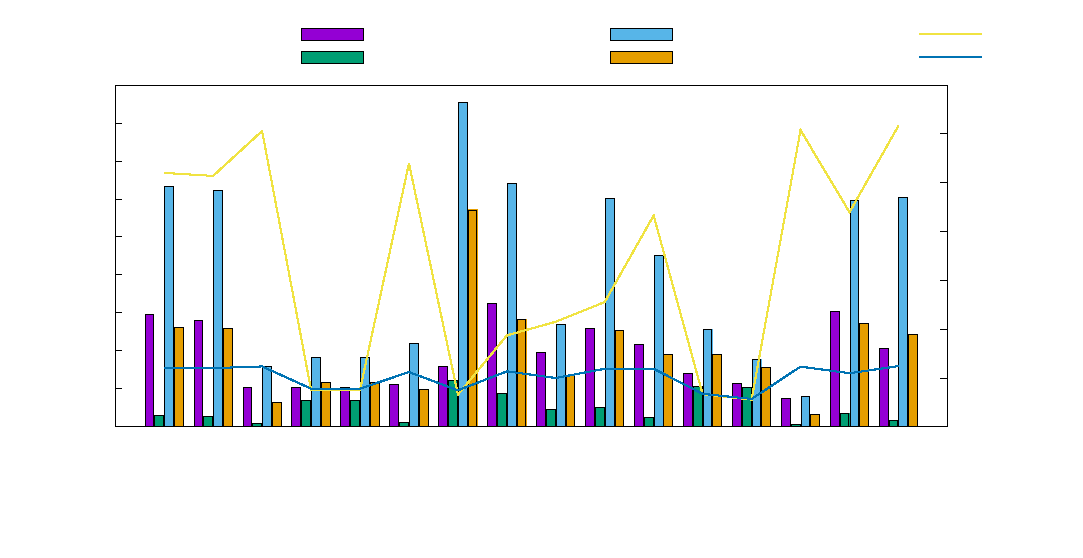
\includegraphics[width={504.00bp},height={252.00bp}]{all-hist-CommunicationMiB}}%
    \gplfronttext
  \end{picture}%
\endgroup

\caption{Communication Size of Benchmarks}
\label{fig:graph_comm_size}
\end{figure*}


\begin{figure*}[htbp]
\centering
% GNUPLOT: LaTeX picture with Postscript
\begingroup
  \makeatletter
  \providecommand\color[2][]{%
    \GenericError{(gnuplot) \space\space\space\@spaces}{%
      Package color not loaded in conjunction with
      terminal option `colourtext'%
    }{See the gnuplot documentation for explanation.%
    }{Either use 'blacktext' in gnuplot or load the package
      color.sty in LaTeX.}%
    \renewcommand\color[2][]{}%
  }%
  \providecommand\includegraphics[2][]{%
    \GenericError{(gnuplot) \space\space\space\@spaces}{%
      Package graphicx or graphics not loaded%
    }{See the gnuplot documentation for explanation.%
    }{The gnuplot epslatex terminal needs graphicx.sty or graphics.sty.}%
    \renewcommand\includegraphics[2][]{}%
  }%
  \providecommand\rotatebox[2]{#2}%
  \@ifundefined{ifGPcolor}{%
    \newif\ifGPcolor
    \GPcolortrue
  }{}%
  \@ifundefined{ifGPblacktext}{%
    \newif\ifGPblacktext
    \GPblacktextfalse
  }{}%
  % define a \g@addto@macro without @ in the name:
  \let\gplgaddtomacro\g@addto@macro
  % define empty templates for all commands taking text:
  \gdef\gplbacktext{}%
  \gdef\gplfronttext{}%
  \makeatother
  \ifGPblacktext
    % no textcolor at all
    \def\colorrgb#1{}%
    \def\colorgray#1{}%
  \else
    % gray or color?
    \ifGPcolor
      \def\colorrgb#1{\color[rgb]{#1}}%
      \def\colorgray#1{\color[gray]{#1}}%
      \expandafter\def\csname LTw\endcsname{\color{white}}%
      \expandafter\def\csname LTb\endcsname{\color{black}}%
      \expandafter\def\csname LTa\endcsname{\color{black}}%
      \expandafter\def\csname LT0\endcsname{\color[rgb]{1,0,0}}%
      \expandafter\def\csname LT1\endcsname{\color[rgb]{0,1,0}}%
      \expandafter\def\csname LT2\endcsname{\color[rgb]{0,0,1}}%
      \expandafter\def\csname LT3\endcsname{\color[rgb]{1,0,1}}%
      \expandafter\def\csname LT4\endcsname{\color[rgb]{0,1,1}}%
      \expandafter\def\csname LT5\endcsname{\color[rgb]{1,1,0}}%
      \expandafter\def\csname LT6\endcsname{\color[rgb]{0,0,0}}%
      \expandafter\def\csname LT7\endcsname{\color[rgb]{1,0.3,0}}%
      \expandafter\def\csname LT8\endcsname{\color[rgb]{0.5,0.5,0.5}}%
    \else
      % gray
      \def\colorrgb#1{\color{black}}%
      \def\colorgray#1{\color[gray]{#1}}%
      \expandafter\def\csname LTw\endcsname{\color{white}}%
      \expandafter\def\csname LTb\endcsname{\color{black}}%
      \expandafter\def\csname LTa\endcsname{\color{black}}%
      \expandafter\def\csname LT0\endcsname{\color{black}}%
      \expandafter\def\csname LT1\endcsname{\color{black}}%
      \expandafter\def\csname LT2\endcsname{\color{black}}%
      \expandafter\def\csname LT3\endcsname{\color{black}}%
      \expandafter\def\csname LT4\endcsname{\color{black}}%
      \expandafter\def\csname LT5\endcsname{\color{black}}%
      \expandafter\def\csname LT6\endcsname{\color{black}}%
      \expandafter\def\csname LT7\endcsname{\color{black}}%
      \expandafter\def\csname LT8\endcsname{\color{black}}%
    \fi
  \fi
    \setlength{\unitlength}{0.0500bp}%
    \ifx\gptboxheight\undefined%
      \newlength{\gptboxheight}%
      \newlength{\gptboxwidth}%
      \newsavebox{\gptboxtext}%
    \fi%
    \setlength{\fboxrule}{0.5pt}%
    \setlength{\fboxsep}{1pt}%
    \definecolor{tbcol}{rgb}{1,1,1}%
\begin{picture}(10080.00,5040.00)%
    \gplgaddtomacro\gplbacktext{%
      \csname LTb\endcsname%%
      \put(814,1540){\makebox(0,0)[r]{\strut{}$0$}}%
      \put(814,1895){\makebox(0,0)[r]{\strut{}$20$}}%
      \put(814,2250){\makebox(0,0)[r]{\strut{}$40$}}%
      \put(814,2605){\makebox(0,0)[r]{\strut{}$60$}}%
      \put(814,2960){\makebox(0,0)[r]{\strut{}$80$}}%
      \put(814,3314){\makebox(0,0)[r]{\strut{}$100$}}%
      \put(814,3669){\makebox(0,0)[r]{\strut{}$120$}}%
      \put(814,4024){\makebox(0,0)[r]{\strut{}$140$}}%
      \put(814,4379){\makebox(0,0)[r]{\strut{}$160$}}%
      \put(1437,1408){\rotatebox{-45}{\makebox(0,0)[l]{\strut{}Biometric Matching}}}%
      \put(1928,1408){\rotatebox{-45}{\makebox(0,0)[l]{\strut{}Convex Hull}}}%
      \put(2419,1408){\rotatebox{-45}{\makebox(0,0)[l]{\strut{}Count 102}}}%
      \put(2910,1408){\rotatebox{-45}{\makebox(0,0)[l]{\strut{}Count 10s}}}%
      \put(3401,1408){\rotatebox{-45}{\makebox(0,0)[l]{\strut{}Cryptonets (Max Pooling)}}}%
      \put(3892,1408){\rotatebox{-45}{\makebox(0,0)[l]{\strut{}Database Join}}}%
      \put(4383,1408){\rotatebox{-45}{\makebox(0,0)[l]{\strut{}Database Variance}}}%
      \put(4875,1408){\rotatebox{-45}{\makebox(0,0)[l]{\strut{}Histogram}}}%
      \put(5366,1408){\rotatebox{-45}{\makebox(0,0)[l]{\strut{}Inner Product}}}%
      \put(5857,1408){\rotatebox{-45}{\makebox(0,0)[l]{\strut{}k-means}}}%
      \put(6348,1408){\rotatebox{-45}{\makebox(0,0)[l]{\strut{}Longest 102}}}%
      \put(6839,1408){\rotatebox{-45}{\makebox(0,0)[l]{\strut{}Max. Dist. b/w Symbols}}}%
      \put(7330,1408){\rotatebox{-45}{\makebox(0,0)[l]{\strut{}Minimal Points}}}%
      \put(7821,1408){\rotatebox{-45}{\makebox(0,0)[l]{\strut{}MNIST ReLU}}}%
      \put(8312,1408){\rotatebox{-45}{\makebox(0,0)[l]{\strut{}Private Set Intersection}}}%
      \put(8935,1540){\makebox(0,0)[l]{\strut{}$0$}}%
      \put(8935,1824){\makebox(0,0)[l]{\strut{}$20$}}%
      \put(8935,2108){\makebox(0,0)[l]{\strut{}$40$}}%
      \put(8935,2392){\makebox(0,0)[l]{\strut{}$60$}}%
      \put(8935,2676){\makebox(0,0)[l]{\strut{}$80$}}%
      \put(8935,2960){\makebox(0,0)[l]{\strut{}$100$}}%
      \put(8935,3243){\makebox(0,0)[l]{\strut{}$120$}}%
      \put(8935,3527){\makebox(0,0)[l]{\strut{}$140$}}%
      \put(8935,3811){\makebox(0,0)[l]{\strut{}$160$}}%
      \put(8935,4095){\makebox(0,0)[l]{\strut{}$180$}}%
      \put(8935,4379){\makebox(0,0)[l]{\strut{}$200$}}%
    }%
    \gplgaddtomacro\gplfronttext{%
      \csname LTb\endcsname%%
      \put(209,2959){\rotatebox{-270}{\makebox(0,0){\strut{}Circuit Generation Time (sec)}}}%
      \put(9573,2959){\rotatebox{-270}{\makebox(0,0){\strut{}Improvement (number of times)}}}%
      \csname LTb\endcsname%%
      \put(2536,4867){\makebox(0,0)[r]{\strut{}GMW}}%
      \csname LTb\endcsname%%
      \put(2536,4647){\makebox(0,0)[r]{\strut{}GMW (Vectorized)}}%
      \csname LTb\endcsname%%
      \put(5503,4867){\makebox(0,0)[r]{\strut{}BMR}}%
      \csname LTb\endcsname%%
      \put(5503,4647){\makebox(0,0)[r]{\strut{}BMR (Vectorized)}}%
      \csname LTb\endcsname%%
      \put(8470,4867){\makebox(0,0)[r]{\strut{}GMW Improvement}}%
      \csname LTb\endcsname%%
      \put(8470,4647){\makebox(0,0)[r]{\strut{}BMR Improvement}}%
    }%
    \gplbacktext
    \put(0,0){\includegraphics[width={504.00bp},height={252.00bp}]{all-hist-CircuitGenerationTimesec}}%
    \gplfronttext
  \end{picture}%
\endgroup

\caption{Circuit Generation Time of Benchmarks}
\label{fig:graph_circ_gen_time}
\end{figure*}

\begin{figure*}[htbp]
\centering
% GNUPLOT: LaTeX picture with Postscript
\begingroup
  \makeatletter
  \providecommand\color[2][]{%
    \GenericError{(gnuplot) \space\space\space\@spaces}{%
      Package color not loaded in conjunction with
      terminal option `colourtext'%
    }{See the gnuplot documentation for explanation.%
    }{Either use 'blacktext' in gnuplot or load the package
      color.sty in LaTeX.}%
    \renewcommand\color[2][]{}%
  }%
  \providecommand\includegraphics[2][]{%
    \GenericError{(gnuplot) \space\space\space\@spaces}{%
      Package graphicx or graphics not loaded%
    }{See the gnuplot documentation for explanation.%
    }{The gnuplot epslatex terminal needs graphicx.sty or graphics.sty.}%
    \renewcommand\includegraphics[2][]{}%
  }%
  \providecommand\rotatebox[2]{#2}%
  \@ifundefined{ifGPcolor}{%
    \newif\ifGPcolor
    \GPcolortrue
  }{}%
  \@ifundefined{ifGPblacktext}{%
    \newif\ifGPblacktext
    \GPblacktextfalse
  }{}%
  % define a \g@addto@macro without @ in the name:
  \let\gplgaddtomacro\g@addto@macro
  % define empty templates for all commands taking text:
  \gdef\gplbacktext{}%
  \gdef\gplfronttext{}%
  \makeatother
  \ifGPblacktext
    % no textcolor at all
    \def\colorrgb#1{}%
    \def\colorgray#1{}%
  \else
    % gray or color?
    \ifGPcolor
      \def\colorrgb#1{\color[rgb]{#1}}%
      \def\colorgray#1{\color[gray]{#1}}%
      \expandafter\def\csname LTw\endcsname{\color{white}}%
      \expandafter\def\csname LTb\endcsname{\color{black}}%
      \expandafter\def\csname LTa\endcsname{\color{black}}%
      \expandafter\def\csname LT0\endcsname{\color[rgb]{1,0,0}}%
      \expandafter\def\csname LT1\endcsname{\color[rgb]{0,1,0}}%
      \expandafter\def\csname LT2\endcsname{\color[rgb]{0,0,1}}%
      \expandafter\def\csname LT3\endcsname{\color[rgb]{1,0,1}}%
      \expandafter\def\csname LT4\endcsname{\color[rgb]{0,1,1}}%
      \expandafter\def\csname LT5\endcsname{\color[rgb]{1,1,0}}%
      \expandafter\def\csname LT6\endcsname{\color[rgb]{0,0,0}}%
      \expandafter\def\csname LT7\endcsname{\color[rgb]{1,0.3,0}}%
      \expandafter\def\csname LT8\endcsname{\color[rgb]{0.5,0.5,0.5}}%
    \else
      % gray
      \def\colorrgb#1{\color{black}}%
      \def\colorgray#1{\color[gray]{#1}}%
      \expandafter\def\csname LTw\endcsname{\color{white}}%
      \expandafter\def\csname LTb\endcsname{\color{black}}%
      \expandafter\def\csname LTa\endcsname{\color{black}}%
      \expandafter\def\csname LT0\endcsname{\color{black}}%
      \expandafter\def\csname LT1\endcsname{\color{black}}%
      \expandafter\def\csname LT2\endcsname{\color{black}}%
      \expandafter\def\csname LT3\endcsname{\color{black}}%
      \expandafter\def\csname LT4\endcsname{\color{black}}%
      \expandafter\def\csname LT5\endcsname{\color{black}}%
      \expandafter\def\csname LT6\endcsname{\color{black}}%
      \expandafter\def\csname LT7\endcsname{\color{black}}%
      \expandafter\def\csname LT8\endcsname{\color{black}}%
    \fi
  \fi
    \setlength{\unitlength}{0.0500bp}%
    \ifx\gptboxheight\undefined%
      \newlength{\gptboxheight}%
      \newlength{\gptboxwidth}%
      \newsavebox{\gptboxtext}%
    \fi%
    \setlength{\fboxrule}{0.5pt}%
    \setlength{\fboxsep}{1pt}%
    \definecolor{tbcol}{rgb}{1,1,1}%
\begin{picture}(10080.00,5040.00)%
    \gplgaddtomacro\gplbacktext{%
      \csname LTb\endcsname%%
      \put(1342,1540){\makebox(0,0)[r]{\strut{}$0$}}%
      \put(1342,2108){\makebox(0,0)[r]{\strut{}$500000$}}%
      \put(1342,2676){\makebox(0,0)[r]{\strut{}$1\times10^{6}$}}%
      \put(1342,3243){\makebox(0,0)[r]{\strut{}$1.5\times10^{6}$}}%
      \put(1342,3811){\makebox(0,0)[r]{\strut{}$2\times10^{6}$}}%
      \put(1342,4379){\makebox(0,0)[r]{\strut{}$2.5\times10^{6}$}}%
      \put(1905,1408){\rotatebox{-45}{\makebox(0,0)[l]{\strut{}Biometric Matching}}}%
      \put(2336,1408){\rotatebox{-45}{\makebox(0,0)[l]{\strut{}Biometric Matching (Fast)}}}%
      \put(2767,1408){\rotatebox{-45}{\makebox(0,0)[l]{\strut{}Convex Hull}}}%
      \put(3198,1408){\rotatebox{-45}{\makebox(0,0)[l]{\strut{}Count 102}}}%
      \put(3630,1408){\rotatebox{-45}{\makebox(0,0)[l]{\strut{}Count 10s}}}%
      \put(4061,1408){\rotatebox{-45}{\makebox(0,0)[l]{\strut{}Cryptonets (Max Pooling)}}}%
      \put(4492,1408){\rotatebox{-45}{\makebox(0,0)[l]{\strut{}Database Join}}}%
      \put(4923,1408){\rotatebox{-45}{\makebox(0,0)[l]{\strut{}Database Variance}}}%
      \put(5354,1408){\rotatebox{-45}{\makebox(0,0)[l]{\strut{}Histogram}}}%
      \put(5785,1408){\rotatebox{-45}{\makebox(0,0)[l]{\strut{}Inner Product}}}%
      \put(6216,1408){\rotatebox{-45}{\makebox(0,0)[l]{\strut{}k-means}}}%
      \put(6647,1408){\rotatebox{-45}{\makebox(0,0)[l]{\strut{}Longest 102}}}%
      \put(7079,1408){\rotatebox{-45}{\makebox(0,0)[l]{\strut{}Max. Dist. b/w Symbols}}}%
      \put(7510,1408){\rotatebox{-45}{\makebox(0,0)[l]{\strut{}Minimal Points}}}%
      \put(7941,1408){\rotatebox{-45}{\makebox(0,0)[l]{\strut{}MNIST ReLU}}}%
      \put(8372,1408){\rotatebox{-45}{\makebox(0,0)[l]{\strut{}Private Set Intersection}}}%
      \put(8935,1540){\makebox(0,0)[l]{\strut{}$0$}}%
      \put(8935,1824){\makebox(0,0)[l]{\strut{}$50$}}%
      \put(8935,2108){\makebox(0,0)[l]{\strut{}$100$}}%
      \put(8935,2392){\makebox(0,0)[l]{\strut{}$150$}}%
      \put(8935,2676){\makebox(0,0)[l]{\strut{}$200$}}%
      \put(8935,2960){\makebox(0,0)[l]{\strut{}$250$}}%
      \put(8935,3243){\makebox(0,0)[l]{\strut{}$300$}}%
      \put(8935,3527){\makebox(0,0)[l]{\strut{}$350$}}%
      \put(8935,3811){\makebox(0,0)[l]{\strut{}$400$}}%
      \put(8935,4095){\makebox(0,0)[l]{\strut{}$450$}}%
      \put(8935,4379){\makebox(0,0)[l]{\strut{}$500$}}%
    }%
    \gplgaddtomacro\gplfronttext{%
      \csname LTb\endcsname%%
      \put(209,2959){\rotatebox{-270}{\makebox(0,0){\strut{}Total Gates}}}%
      \put(9573,2959){\rotatebox{-270}{\makebox(0,0){\strut{}Improvement (number of times)}}}%
      \csname LTb\endcsname%%
      \put(2800,4867){\makebox(0,0)[r]{\strut{}GMW}}%
      \csname LTb\endcsname%%
      \put(2800,4647){\makebox(0,0)[r]{\strut{}GMW (Vectorized)}}%
      \csname LTb\endcsname%%
      \put(5767,4867){\makebox(0,0)[r]{\strut{}BMR}}%
      \csname LTb\endcsname%%
      \put(5767,4647){\makebox(0,0)[r]{\strut{}BMR (Vectorized)}}%
      \csname LTb\endcsname%%
      \put(8734,4867){\makebox(0,0)[r]{\strut{}GMW Improvement}}%
      \csname LTb\endcsname%%
      \put(8734,4647){\makebox(0,0)[r]{\strut{}BMR Improvement}}%
    }%
    \gplbacktext
    \put(0,0){\includegraphics[width={504.00bp},height={252.00bp}]{all-hist-TotalGates}}%
    \gplfronttext
  \end{picture}%
\endgroup

\caption{Number of Gates of Benchmarks}
\label{fig:graph_total_gates}
\end{figure*}

\begin{figure*}[htbp]
\centering
\input{graphs/lan/all-hist-OnlineTimesec}
\caption{Online Time of Benchmarks}
\label{fig:graph_online_time}
\end{figure*}

\begin{figure*}[htbp]
\centering
% GNUPLOT: LaTeX picture with Postscript
\begingroup
  \makeatletter
  \providecommand\color[2][]{%
    \GenericError{(gnuplot) \space\space\space\@spaces}{%
      Package color not loaded in conjunction with
      terminal option `colourtext'%
    }{See the gnuplot documentation for explanation.%
    }{Either use 'blacktext' in gnuplot or load the package
      color.sty in LaTeX.}%
    \renewcommand\color[2][]{}%
  }%
  \providecommand\includegraphics[2][]{%
    \GenericError{(gnuplot) \space\space\space\@spaces}{%
      Package graphicx or graphics not loaded%
    }{See the gnuplot documentation for explanation.%
    }{The gnuplot epslatex terminal needs graphicx.sty or graphics.sty.}%
    \renewcommand\includegraphics[2][]{}%
  }%
  \providecommand\rotatebox[2]{#2}%
  \@ifundefined{ifGPcolor}{%
    \newif\ifGPcolor
    \GPcolortrue
  }{}%
  \@ifundefined{ifGPblacktext}{%
    \newif\ifGPblacktext
    \GPblacktextfalse
  }{}%
  % define a \g@addto@macro without @ in the name:
  \let\gplgaddtomacro\g@addto@macro
  % define empty templates for all commands taking text:
  \gdef\gplbacktext{}%
  \gdef\gplfronttext{}%
  \makeatother
  \ifGPblacktext
    % no textcolor at all
    \def\colorrgb#1{}%
    \def\colorgray#1{}%
  \else
    % gray or color?
    \ifGPcolor
      \def\colorrgb#1{\color[rgb]{#1}}%
      \def\colorgray#1{\color[gray]{#1}}%
      \expandafter\def\csname LTw\endcsname{\color{white}}%
      \expandafter\def\csname LTb\endcsname{\color{black}}%
      \expandafter\def\csname LTa\endcsname{\color{black}}%
      \expandafter\def\csname LT0\endcsname{\color[rgb]{1,0,0}}%
      \expandafter\def\csname LT1\endcsname{\color[rgb]{0,1,0}}%
      \expandafter\def\csname LT2\endcsname{\color[rgb]{0,0,1}}%
      \expandafter\def\csname LT3\endcsname{\color[rgb]{1,0,1}}%
      \expandafter\def\csname LT4\endcsname{\color[rgb]{0,1,1}}%
      \expandafter\def\csname LT5\endcsname{\color[rgb]{1,1,0}}%
      \expandafter\def\csname LT6\endcsname{\color[rgb]{0,0,0}}%
      \expandafter\def\csname LT7\endcsname{\color[rgb]{1,0.3,0}}%
      \expandafter\def\csname LT8\endcsname{\color[rgb]{0.5,0.5,0.5}}%
    \else
      % gray
      \def\colorrgb#1{\color{black}}%
      \def\colorgray#1{\color[gray]{#1}}%
      \expandafter\def\csname LTw\endcsname{\color{white}}%
      \expandafter\def\csname LTb\endcsname{\color{black}}%
      \expandafter\def\csname LTa\endcsname{\color{black}}%
      \expandafter\def\csname LT0\endcsname{\color{black}}%
      \expandafter\def\csname LT1\endcsname{\color{black}}%
      \expandafter\def\csname LT2\endcsname{\color{black}}%
      \expandafter\def\csname LT3\endcsname{\color{black}}%
      \expandafter\def\csname LT4\endcsname{\color{black}}%
      \expandafter\def\csname LT5\endcsname{\color{black}}%
      \expandafter\def\csname LT6\endcsname{\color{black}}%
      \expandafter\def\csname LT7\endcsname{\color{black}}%
      \expandafter\def\csname LT8\endcsname{\color{black}}%
    \fi
  \fi
    \setlength{\unitlength}{0.0500bp}%
    \ifx\gptboxheight\undefined%
      \newlength{\gptboxheight}%
      \newlength{\gptboxwidth}%
      \newsavebox{\gptboxtext}%
    \fi%
    \setlength{\fboxrule}{0.5pt}%
    \setlength{\fboxsep}{1pt}%
    \definecolor{tbcol}{rgb}{1,1,1}%
\begin{picture}(10080.00,5040.00)%
    \gplgaddtomacro\gplbacktext{%
      \csname LTb\endcsname%%
      \put(814,1540){\makebox(0,0)[r]{\strut{}$0$}}%
      \put(814,2013){\makebox(0,0)[r]{\strut{}$50$}}%
      \put(814,2486){\makebox(0,0)[r]{\strut{}$100$}}%
      \put(814,2960){\makebox(0,0)[r]{\strut{}$150$}}%
      \put(814,3433){\makebox(0,0)[r]{\strut{}$200$}}%
      \put(814,3906){\makebox(0,0)[r]{\strut{}$250$}}%
      \put(814,4379){\makebox(0,0)[r]{\strut{}$300$}}%
      \put(1445,1408){\rotatebox{-45}{\makebox(0,0)[l]{\strut{}Biometric Matching}}}%
      \put(1945,1408){\rotatebox{-45}{\makebox(0,0)[l]{\strut{}Convex Hull}}}%
      \put(2444,1408){\rotatebox{-45}{\makebox(0,0)[l]{\strut{}Count 102}}}%
      \put(2943,1408){\rotatebox{-45}{\makebox(0,0)[l]{\strut{}Count 10s}}}%
      \put(3443,1408){\rotatebox{-45}{\makebox(0,0)[l]{\strut{}Cryptonets (Max Pooling)}}}%
      \put(3942,1408){\rotatebox{-45}{\makebox(0,0)[l]{\strut{}Database Join}}}%
      \put(4441,1408){\rotatebox{-45}{\makebox(0,0)[l]{\strut{}Database Variance}}}%
      \put(4941,1408){\rotatebox{-45}{\makebox(0,0)[l]{\strut{}Histogram}}}%
      \put(5440,1408){\rotatebox{-45}{\makebox(0,0)[l]{\strut{}Inner Product}}}%
      \put(5939,1408){\rotatebox{-45}{\makebox(0,0)[l]{\strut{}k-means}}}%
      \put(6438,1408){\rotatebox{-45}{\makebox(0,0)[l]{\strut{}Longest 102}}}%
      \put(6938,1408){\rotatebox{-45}{\makebox(0,0)[l]{\strut{}Max. Dist. b/w Symbols}}}%
      \put(7437,1408){\rotatebox{-45}{\makebox(0,0)[l]{\strut{}Minimal Points}}}%
      \put(7936,1408){\rotatebox{-45}{\makebox(0,0)[l]{\strut{}MNIST ReLU}}}%
      \put(8436,1408){\rotatebox{-45}{\makebox(0,0)[l]{\strut{}Private Set Intersection}}}%
      \put(9067,1540){\makebox(0,0)[l]{\strut{}$0$}}%
      \put(9067,1946){\makebox(0,0)[l]{\strut{}$5$}}%
      \put(9067,2351){\makebox(0,0)[l]{\strut{}$10$}}%
      \put(9067,2757){\makebox(0,0)[l]{\strut{}$15$}}%
      \put(9067,3162){\makebox(0,0)[l]{\strut{}$20$}}%
      \put(9067,3568){\makebox(0,0)[l]{\strut{}$25$}}%
      \put(9067,3973){\makebox(0,0)[l]{\strut{}$30$}}%
      \put(9067,4379){\makebox(0,0)[l]{\strut{}$35$}}%
    }%
    \gplgaddtomacro\gplfronttext{%
      \csname LTb\endcsname%%
      \put(209,2959){\rotatebox{-270}{\makebox(0,0){\strut{}Setup Time (sec)}}}%
      \put(9573,2959){\rotatebox{-270}{\makebox(0,0){\strut{}Improvement (number of times)}}}%
      \csname LTb\endcsname%%
      \put(2602,4867){\makebox(0,0)[r]{\strut{}GMW}}%
      \csname LTb\endcsname%%
      \put(2602,4647){\makebox(0,0)[r]{\strut{}GMW (Vectorized)}}%
      \csname LTb\endcsname%%
      \put(5569,4867){\makebox(0,0)[r]{\strut{}BMR}}%
      \csname LTb\endcsname%%
      \put(5569,4647){\makebox(0,0)[r]{\strut{}BMR (Vectorized)}}%
      \csname LTb\endcsname%%
      \put(8536,4867){\makebox(0,0)[r]{\strut{}GMW Improvement}}%
      \csname LTb\endcsname%%
      \put(8536,4647){\makebox(0,0)[r]{\strut{}BMR Improvement}}%
    }%
    \gplbacktext
    \put(0,0){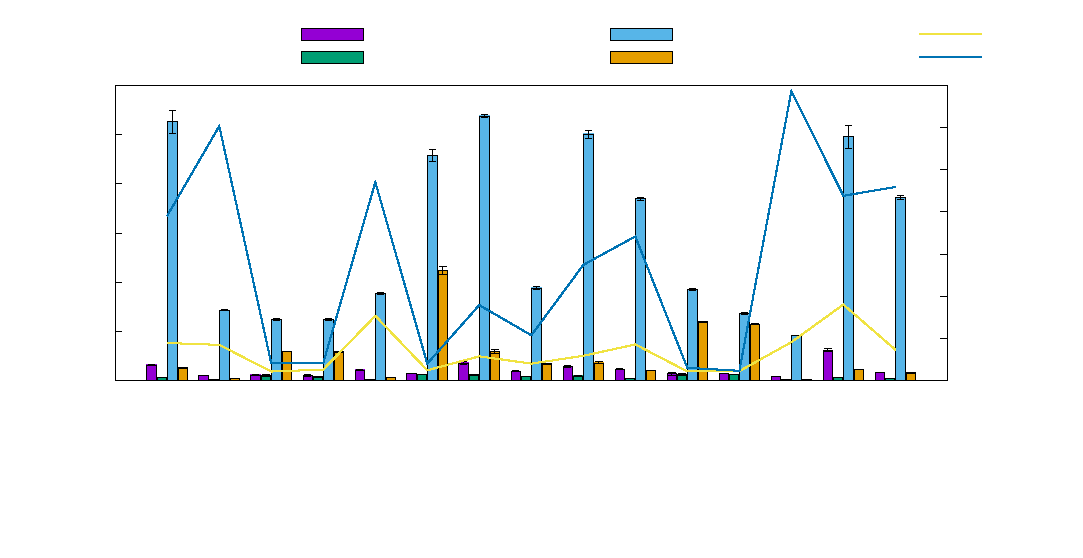
\includegraphics[width={504.00bp},height={252.00bp}]{all-hist-SetupTimesec}}%
    \gplfronttext
  \end{picture}%
\endgroup

\caption{Setup Time of Benchmarks}
\label{fig:graph_setup_time}
\end{figure*}

\subsection{Discussion}
\ana{Ana todo: Discuss why we are slower than HyCC --- because of ad-hoc div-and-conquer optimizations. Have to summarize what Ben and I figured out yesterday.}

\ana{If we can add that our cost model works great (it does!), that would be great but probably won't have time...}


%\end{document}

%%% Local Variables: 
%%% mode: latex
%%% TeX-master: t
%%% End: 

%\include{chapterfive}
%\include{chaptersix}
%%%%%%%%%%%%%%%%%%%%%%%%%%%%%%%%%%%%%%%%%%%%%%%%%%%%%%%%%%%%%%%%%%% 
%                                                                 %
%                           BIBLIOGRAPHY                          %
%                                                                 %
%%%%%%%%%%%%%%%%%%%%%%%%%%%%%%%%%%%%%%%%%%%%%%%%%%%%%%%%%%%%%%%%%%% 
 
%This method produces a numbered bibliography where the numbers
%correspond to the \cite commands in the text. See the LaTeX manual.
%
% \specialhead{REFERENCES}
% \begin{singlespace}
% \begin{thebibliography}{99}
% \bibitem{thisbook} This is the first item in the Bibliography.
% Let's make it very long so it takes more than one line.
% Let's make it very long so it takes more than one line.
% Let's make it very long so it takes more than one line.
% Let's make it very long so it takes more than one line. 
% \bibitem{anotherbook} The second item in the Bibliography.
% \bibitem{yetanotherbook} Another item in the Bibliography.
% \end{thebibliography}
% \end{singlespace}
\addcontentsline{toc}{chapter}{REFERENCES}
% \specialhead{REFERENCES}
\bibliographystyle{myIEEETran} % specify bibliography style
% \begin{singlespace}
\raggedright
\bibliography{library} % Prints the bibliography here, using "myrefs.bib"
% \end{singlespace}

% \bibliographystyle{acm}
% \bibliography{library}

% Note that, if you wish, you can use BibTeX to create your bibliography
% from a database. See section 5.6.2 of Memo RPI.110 for information. 
%%% Local Variables: 
%%% mode: latex
%%% TeX-master: t
%%% End: 
 % bibliography
% \include{appendix} % appendix
 
\end{document}
